\documentclass[11pt,twoside]{starlink}

% -----------------------------------------------------------------------------
% ? Document identification
\stardoccategory    {Starlink Cookbook}
\stardocinitials    {SC}
\stardocsource      {sc\stardocnumber}
\stardocnumber      {8.1}
\stardocauthors     {Henry Matthews, Tim Jenness}
\stardocdate        {1st March 1997}
\stardoctitle       {Specx Cookbook \\[\latex{2ex}]
                                Reduction of millimetre wave data}
\startitlepic{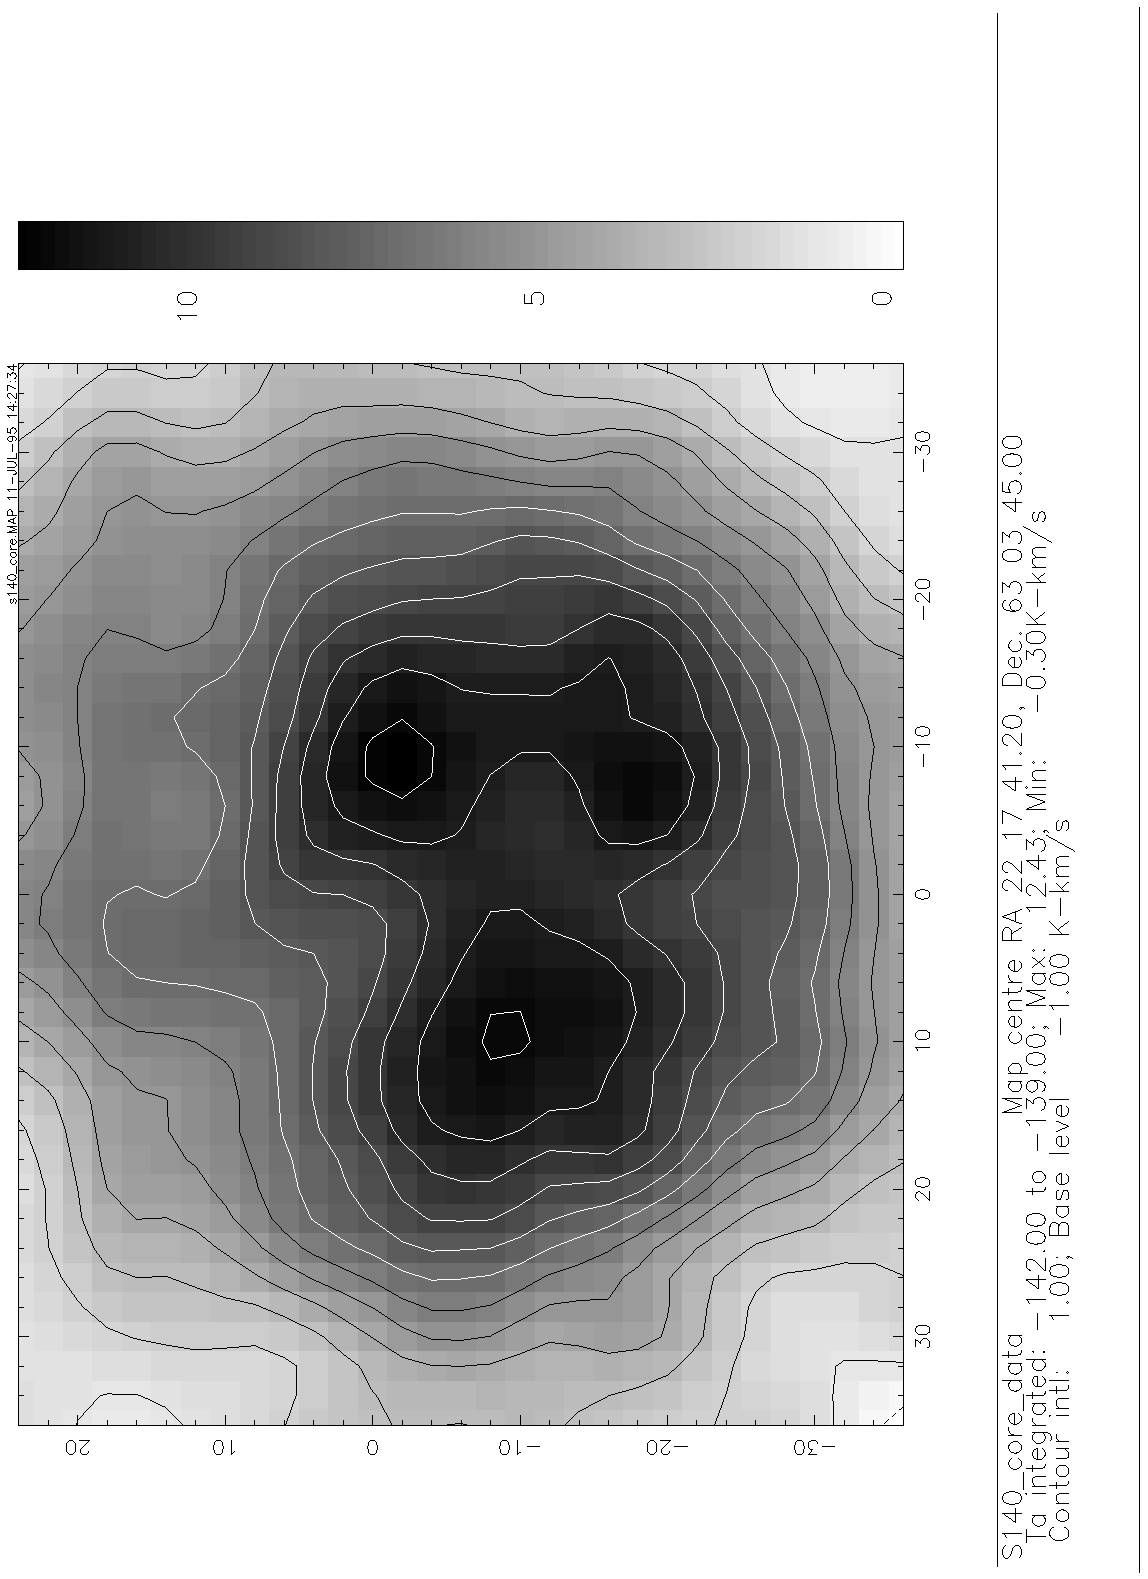
\includegraphics[width=0.7\textwidth]{sc8_gray}}
\stardocabstract  {%
This cookbook provides an introduction to the facilities
found in the SPECX data reduction package.
}
% ? End of document identification

% -----------------------------------------------------------------------------

% ? Document specific \providecommand or \newenvironment commands.

\providecommand{\scspec}[2]{#1}

\renewcommand{\topfraction}{1.0}
\renewcommand{\bottomfraction}{1.0}
\renewcommand{\floatpagefraction}{0.9}
\renewcommand{\textfraction}{0.01}

%%%%%%  DEFINE SOME COMMANDS
% This is COMMANDS.TEX
\renewcommand{\textfraction}{0.1}
\providecommand{\etal}{\textit{et.~al.}}
\providecommand{\eg}{\textit{e.g.}}
\providecommand{\ie}{\textit{i.e.}}
\providecommand{\arcsec}{$''$}
\providecommand{\arcmin}{$'$}
\providecommand{\micron}{$\mu$m}
\providecommand{\degr}{$^\circ$}
\providecommand{\kps}{km sec$^{-1}$}
\providecommand{\lsun}{L$_\odot$}
\providecommand{\msun}{M$_\odot$}
\providecommand{\msundot}{M$_\odot$ yr$^{-1}$}
\providecommand{\Clower}{C{\small I}($^3$P$_1$--$^3$P$_0$)}
\providecommand{\Cupper}{C{\small I}($^3$P$_2$--$^3$P$_1$)}
\providecommand{\lb}{$\ell$/b}
\providecommand{\yes}{$\heartsuit$}
\providecommand{\SCUBA}{\textit{SCUBA}}
\providecommand{\scuba}{\textit{SCUBA}}
\providecommand{\SPECX}{\texttt{SPECX}}
%\providecommand{\UKT14}{\texttt{UKT14}}
\providecommand{\das}{\texttt{DAS}}
\providecommand{\aosc}{\texttt{AOSC}}
\providecommand{\apj}{\textit{Astrophys.\ J.}}
\providecommand{\aj}{\textit{Astron.\ J.}}
\providecommand{\apjlett}{\textit{Astrophys.\ J.\ (Letters)}}
\providecommand{\apjsupp}{\textit{Astrophys.\ J.\ Suppl.}}
\providecommand{\austjsupp}{\textit{Aust.\ J.\ Phys.\ Suppl.}}
\providecommand{\aanda}{\textit{Astron.\ Astrophys.}}
\providecommand{\aasupp}{\textit{Astron.\ Astrophys.\ Suppl.}}
\providecommand{\nature}{\textit{Nature}}
\providecommand{\mnras}{\textit{Mon. Not. Roy. astr. Soc.}}
\providecommand{\annrev}{\textit{Ann.\ Rev.\ Astron.\ Astrophys.}}
\providecommand{\pasp}{\textit{Pub.\ Astron.\ Soc.\ Pacific}}
\providecommand{\revmex}{\textit{Rev.\ Mex.\ Astr.\ Astrofiz.}}
\providecommand{\dm}{\texttt{das-merge}}

\providecommand{\margnote}[1]
{\marginpar{({\it{\ref{#1}}})}}

\normalmarginpar
\providecommand{\SP}{{$>\!>$}}

\newenvironment{aside}{
\begin{quote}\begin{center}\rule[1mm]{1.0in}{0.015in}\hspace*{2mm}
\textbf{An Aside}
\hspace*{2mm}\rule[1mm]{1.0in}{0.015in}\end{center}
}{
\myline
\end{quote}
}

\providecommand{\myline}
{\vspace*{-0.2in}\begin{center}\rule{3.0in}{0.015in}\end{center}}

\providecommand{\ctrlc}{\texttt{Control-c}}
\providecommand{\ctrld}{\texttt{Control-d}}
\providecommand{\ctrlz}{\texttt{Control-z}}

% ? End of document specific commands
% -----------------------------------------------------------------------------
%  Title Page.
%  ===========

\begin{document}
\scfrontmatter

\section{\xlabel{a_specx_cookbook}A \SPECX\ ``Cookbook''}
\label{sec:specx-cookbook}
\SPECX\ is a versatile spectral line data reduction package written by Rachael
Padman (Cavendish Laboratory, Cambridge, U.K), and supported also by
Starlink and local effort at the Joint Astronomy Centre in Hilo,
Hawaii.  It is made available to all users at the JCMT, and a
standalone version can be downloaded from the JCMT home page on the
Web.\footnote{Contact Tim Jenness at the JAC in the first instance
regarding this implementation of
\SPECX , if you want to, say, install it at your home institution. The
UNIX version may be downloaded from the JCMT Web page; please register
using the form given there if you decide to go this way.}

This guide (``Cookbook'', perhaps) was first written long
ago\footnote{The first version of this section appeared as the `SPECX
Cookbook' and was written by Thomas Walker. He moved on to greater
things, but still accepts accolades and greenbacks at
\texttt{walker@stsci.edu}.} to help the novice
\SPECX\ user get a spectrum on the screen and do some simple data reduction.
The original aim is preserved in this version: it is not meant to be a
complete manual on all the facets of \SPECX ; the definitive words on
any topic contained in this section will be found in the full \SPECX\
manual, written by Rachael Padman, and which should be readily to hand
at the JCMT, Hale Pohaku, and at the JAC.  For questions regarding the
way \SPECX\ works, the staff scientist assigned to support your
observing run should be able to assist in the more mundane `how-to'
questions; don't bother the software group with these. This
``Cookbook'' is available on the WWW in Postscript and HTML at
\url{http://www.jach.hawaii.edu/JCMT/astroman/}. It is likely that the
Web versions will be more up-to-date than any printed version.

\begin{quote}
\begin{center}
\fbox{
\begin{minipage}[t]{0.8\textwidth}
\textbf{Note:} \SPECX\ is currently in version 6.7; at JAC this is the
version installed under Unix, while only version 6.3 is available on
VMS platforms.  Version 7.0 is rumoured to be in the works.  This
``cookbook'' deals primarily with version 6.7 under Unix
There are a considerable number of changes in this release which
make previous documentation obsolete, including older versions of this
Cookbook.  Older documentation should be discarded. This Cookbook is
not intended to be a complete description of \SPECX . As far as I am
aware there is no complete up-to-date manual for \SPECX\ right now,
the last being for version 6.3.
\end{minipage}
}
\end{center}
\end{quote}

\section{\xlabel{rapid_introduction_to_specx}Rapid Introduction to \SPECX }
\label{sec:rapid-specx}
Let's assume you just got your data from the telescope;
now you need to
look at the data, but don't want to read the \SPECX\ manual or this
one. Then follow these steps, depending on what you want to do. You
can learn about the intricacies later. Occasional margin notes, like
the one here\margnote{sec:specx-intro}, indicate sections where
additional information can be found in the main part of this
`Cookbook'.

\subsection{Start-up}
\label{sec:start-up}
\margnote{sec:finding-the-data}

Starting \SPECX\ is simple. All the necessary environment variables should
have been setup correctly as part of your Starlink login.
You can start \SPECX\ from any directory in which you have write access but
for now it's easier if you start it up in the directory that contains your
data. In order to start \SPECX\, type:

\begin{terminalv}
% specx
\end{terminalv}
\reversemarginpar
The \texttt{\%} sign represents the shell prompt for input; its actual
form may be something Unix-y like \verb@3:45|iiwi~|@; in this case
giving the time and a reminder of the name of the workstation you are
logged into.

\SPECX\ will next dump out part of a long introductory
text. You might want to read this; if so use the space bar to jump a
page at a time. If not, use \ctrlc\ to jump to the end. At the end,
the system responds with the \SPECX\ prompt:

\SP

\begin{aside}
If \SPECX\ complains that it cannot find your data, this is likely
if you started \SPECX\ in a directory that does not contain your data,
you
should exit \SPECX\ (using the command {\tt{exit}}), and before
restarting up \SPECX\ type e.g.:

\begin{terminalv}
% setenv DATADIR /data/m96bc05/
\end{terminalv}

or wherever you happen to have stored your data. \SPECX\ will then
look for data first in your current directory but then in your data
directory (as defined by the DATADIR environment variable).

\end{aside}

\subsection{Initialization}
\label{sec:specx-init}
\margnote{sec:preparing-specx}
Check, and perhaps set, terminal device,
plot device, and hardcopy device. Generally the defaults will be what
you want, but it won't hurt to go through the motions:

\SP\ {\tt{s-t-d}} \hspace*{0.5in}(system default is {\tt{xw}} for a
Sun workstation such as {\tt{IIWI}})

\SP\ {\tt{s-p-d t}} \hspace*{0.35in}(set to plot on terminal screen)

\SP\ {\tt{s-h-d}} \hspace*{0.5in}(default is Postscript-landscape --
shown as {\verb|ps_l|}; but note alternatives)

The default state of \SPECX\ is to look for spectra taken with the
\das ; if that's what you want, there is no need to do anything to get
it. However, if you have (old) data taken with the \aosc , say, a
number of parameters have to be changed. See
Section~\ref{sec:preparing-specx} for this and other additional
information on setting up \SPECX .

\normalmarginpar
\subsection{Looking at spectra}
To read in a spectrum (GSD format)\margnote{sec:getting-the-data} type
(\eg\ spectrum 131):

\SP\ {\tt{r-g-d 131}}

See Section~\ref{sec:getting-the-data} for more information,
especially if you want to look at map data.

Plot on screen:

\SP\ {\tt{n}}

Incidentally, \das\ spectra do not look very pretty (cf.
Figure~\ref{fig:dm_dirty}) in most cases at this point until you have
done the step described in section~\ref{sec:subbands}. \SPECX\ under
Unix also has a bad habit of leaving the cursor on the plot window.

Change plot scales\margnote{sec:specx_5.1} with:

\SP\ {\tt{s-p-sc}}

and answer the questions.

The x-axis default is {\it{velocity}}; if you want to change it
use\margnote{sec:set-x}:

\SP\ {\tt{set-x}}

and complete the dialog. The basic options are channels, velocity and
frequency scales.


\subsection{Averaging spectra}
To average\margnote{sec:specx_8.2} three spectra (131, 132 and 133) type:

\SP\ {\tt{r-g-d 131}}\\
\SP\ {\tt{r-g-d 132; ave}}\\
\SP\ {\tt{r-g-d 133; ave}}

Plot result, with

\SP\ {\tt{n}}

Incidentally, note that two or more commands may be placed on one
line, separated by semicolons, as shown in this example.

\subsection{Dealing with \das\ spectra: basics}
\label{sec:subbands}
As described elsewhere,
\das\ spectra usually
\margnote{sec:das-merge}
consist of several overlapping (in frequency/velocity space) sections
(or `sub-bands'). Except for single sub-band (125-MHz) spectra it is
necessary to combine these sub-bands to produce a nice spectrum. This
is done with the command {\tt{das-merge}}; \eg :

\SP\ \texttt{r-g-d 131; das-merge}

This command removes the large data values at the ends
of the subbands, and combines the subbands into one continuous
spectum.  It is sufficient to take the defaults for most purposes;
however, see Section~\ref{sec:das-merge} for caveats etc.  The final
spectrum should be free of evidence of sub-band edges, except in
pathological cases.

%Note that in the current version of \SPECX\ the horizontal
%plot scale is reset.

\reversemarginpar
Note that:
\begin{itemize}
\item
It is not necessary to do the \texttt{das-merge} operation on individual
spectra before averaging; the average can be formed first and
{\tt{das-merge}} applied to the result.
\item
If you have modified the centre frequency of the previous spectrum
\margnote{sec:s-l-r-f}
using the {\tt{s-l-r-f}} command\footnote{More on this in
Section~\ref{sec:s-l-r-f}.} it is necessary to reset the defaults
using

\SP\ {\tt{s-l-r-f 0.0}}

before attempting the {\tt{das-merge}} command.
\end{itemize}

\subsection{Sending plots to laser printer}
The \margnote{sec:specx_12} simplest way is to type

\SP\ {\tt{laser}}

to send the last plot you made on the screen. The Unix version of
\SPECX\ creates a plot file called \verb|specx_pgplot.ps| if you have
asked for Postscript files to be made (these are the required type for
our normal printer). This plot file will be overwritten every time you
issue a new plot command.

To send any other plot directly to the (laser) printer, first change plot
device to {\tt{hardcopy}}:

\SP\ {\tt{s-p-d h}}

then open a new plotfile:

\SP\ {\tt{n}}

and {\it{either}} close the plotfile;

\SP\ {\tt{cl-pl}}

\textit{or} open a new plotfile;

\SP\ {\tt{n}}

{\it{or}} reset the plot device:

\SP\ {\tt{s-p-d t}}

all of which create the plotfile \verb|specx_pgplot.ps|.
To plot it on the default (local) printer use

\SP\ \verb|$ lp specx_pgplot.ps|

and if you like this plot enough you can save the Postscript file with

\SP\ \verb|$ mv specx_pgplot.ps| {\it{yourplotfilename}}{\tt{.ps}}

\normalmarginpar
\subsection{Saving the results}
Data may be written to {\it{files}}, which can contain many spectra, or
saved temporarily in {\it{storage registers}}, each of which contains
only one spectrum.

To write data to a file, first open one\margnote{sec:data-files}:

\SP\ {\tt{o-fil}}

and tell \SPECX\ the file name etc\footnote{The VMS version of \SPECX\
requires the number of spectra expected in addition; Unix allows the
files to be expanded indefinitely.}. Each file can be addressed by its
name, or a number. A file name has by default the filetype {\tt{.sdf}},
which will be added to whatever name you give. Several files may be
open at once. To discover a file's number (you will need this) type:

\SP\ {\tt{l-o-f}}

Then, to write the current data (that seen with the {\tt{n}} command)
to (say) file 2 type:

\SP\ {\tt{wr-sp 2}}

The data are stored in the next available space.

To list the contents of a file type:

\SP\ {\tt{ind-fil}}

and answer the questions.

To save the current data in a temporary storage
register\margnote{sec:temp-storage}, type, e.g.:

\SP\ {\tt{st-sp 3}}

\subsection{Retrieving data}
To read data from file you must have read ({\tt{R}}), or read-write
({\tt{RW}}), access. The default state of newly-created files is
write-only. {\tt{l-o-f}} will tell you the current access. To
change the latter enter\margnote{sec:data-files}:

\SP\ {\tt{s-f-a}}

and answer the questions.

To read a spectrum (say, number 16, from file 2):

\SP\ {\tt{rea-s 2 16}}

This places the result in the x-register, from where it is immediately
available for plotting or whatever you might have in mind.

To get data from a temporary storage area\margnote{sec:temp-storage} (say, 3):

\SP\ {\tt{reca-sp 3}}

\subsection{Fitting and removing baselines}
\reversemarginpar
One usually finds that one's spectral line lies atop some kind of
baseline curvature; to display the line to better advantage one fits a
linear, polynomial or other function to the line-free regions of the
spectrum. It is possible to specify the ``fit regions'' either by
typing in the numbers, or by using the cursor with the plot.
The latter is where the interactive mode comes in handy. First type:

\SP\ {\tt{set-int y}}

Then use\margnote{sec:linear-baselines}

\SP\ {\tt{r-l-b}}

to remove a {\it{linear}} baseline from the current spectrum. Define
{\it{two}} fitting regions by placing the cursor in the respective
positions, and typing {\tt{l}}, {\tt{r}}, and {\tt{a}} (left, right,
accept, region) for each. The x-register will contain the result.

To remove a polynomial baseline, type\margnote{sec:poly-baselines}

\SP\ {\tt{f-p-b}}

and define a number of regions to which the baseline is to be
fitted. If you use the cursor as before, exit the plot screen with an
`{\tt{e}}' (for `exit'). If you supply the fit ranges in
non-interactive mode terminate the entries with \ctrld
.\footnote{\SPECX\ prompts you for an `{\tt{EOF}}' (end-of-file);
what the Unix-types don't tell you is that this is a \ctrld ; it is
\ctrlz\ under VMS.} Next you will be prompted for the order of polynomial to
be fitted. The model fit curve is in the x-register and the original
data in the y-register.\footnote{\SPECX\ uses an HP calculator-like
stack; the x-register is on the top, and is the one which is always
plotted.}

Then to display the fit superposed on the original before subtraction,
type, say

\SP\ {\tt{over 1 5}}

The overlay function expects two numbers -- the line width and colour.

Generally you will be confident of the results of your fit, so you can
skip the above step. To see the final baseline-subtracted result type

\SP\ {\tt{sub; n}}

\subsection{Making maps}
Map files\margnote{sec:specx_13} (`datacubes' to the initiated)
consist of a potentially large number of related spectra in one place
under a common header. The spectra are taken on a regular spatial grid
of points. This, and a few other things, you must tell \SPECX\ before
anything else. First create a map file with

\SP\ {\tt{o-map}}

Give it a name (whatever name you give is automatically appended with
the string {\tt{\_map.sdf}}), tell the system the grid spacing of the
observations, and a few other things (answer the questions). Be sure
to set the map size to be adequate for your needs, or else you will
have to recreate it later. Only one map file may be open at one time.

To place the current spectrum in the map file, use the {\tt{add-to-map}}
command\margnote{sec:specx_13.2}:

\SP\ {\tt{a-t-m}}

\normalmarginpar
To overwrite an existing spectrum in the map, first use

\SP\ {\tt{s-m-a}}

to set map access (or not, as the case may be).

\subsection{Displaying Map Data}
Several techniques are useful. First, typing\margnote{sec:specx_13.3}

\SP\ \texttt{gr-sp}

will display a set of postage-stamp spectra on the page. You provide a
number of parameters defining the plot.

Second, use\margnote{sec:specx_13.4}

\SP\ \texttt{cont}

to obtain a contour plot.

Or, better yet (provided you are working on a Sun workstation or
something similar), type\margnote{sec:grayscale}

\SP\ \texttt{gray}

to obtain a gray-scale plot. This can be turned into various colour
schemes, with a number of options. I suggest you experiment; using the
interactive mode is a good way to do this -- type `{\tt{h}}' within the
plot to see the options available -- or in non-interactive mode use
the command

\SP\ \texttt{set-gray}

Finally, either using \texttt{s-p-d h} and sending one of the above
commands, or typing \texttt{see-map}, will save the image to a file
(\eg\ {\tt{specx\_pgplot.ps}}) suitable for output to the printer.

\subsection{Some other things}
Any command may be aborted while it awaits input by typing \ctrlc .

Data may be `binned' (averaged) over \textit{n} channels by typing

\SP\ \texttt{bin} \textit{n}

and smoothed using

\SP\ \texttt{hann}

Several spectra may be plotted on the same frame to good effect by
offsetting vertically with respect to one another using

\SP\ \texttt{off-sp}

and then using the \texttt{over} command.

One spectrum may be subtracted from another by using

\SP\ \texttt{sub}

or divided by another (channel-by-channel) by typing:

\SP\ \texttt{f-q-s}

\subsection{And now\ldots}
This just gets you started. By now you should have learned enough for
simple operations. However, like as not you will want more, such as how
to build procedures for repetitive operations. So, you will have to
read the full introduction to \SPECX\ in this cookbook, or Rachael
Padman's full \SPECX\ manual. Also, experimentation is a good thing;
the worst that can happen is a core dump (a large file called \texttt{core} will be created in your directory). You should delete this file
if this happens.

%%%%%%%%%%%%%%%%%%

\section{\xlabel{a_more_complex_introdcution_to_specx}%
A More Complete Introduction to \SPECX }
\label{sec:specx-intro}

\SPECX\ should be run on a graphics-capable terminal for full use of its
capabilities; at the JCMT and elsewhere the preferred device is a Sun
workstation. Alternatives are other Xwindow devices (such as DECstation
4000's and VXT2000's) and `dumb terminals' like VT330's. Plot display
can be redirected as required to these devices. If you don't want to
plot you can run \SPECX\ on a non-graphics terminal (\eg\ a VT220).


\subsection{Finding your data}
\label{sec:finding-the-data}

\SPECX\ can read data from data directories that are distinct from your
working directory. This leads to directories that are far less cluttered than
would otherwise be the case. \SPECX\ does this by using the DATADIR
environment variable. When a \texttt{read-gsd-data} or \texttt{read-gsd-raster}
command is issued \SPECX\ searches for the GSD file in the current directory
and, if the file can not be found, then in the directory specified by
DATADIR.

For example, if you stored your data in /data/jcmtrun then you would issue the
following command before starting \SPECX:

\begin{terminalv}
% setenv DATADIR /data/jcmtrun
\end{terminalv}

Now when \SPECX\ is started, the directory /data/jcmtrun will be used as
a GSD data directory. You are then ready to start up \SPECX .

\subsection{Getting into \SPECX }
\label{sec:starting-specx}
After you have found your data, and optionally re-directed the plot
output (above), give the following command:

\begin{terminalv}
% specx
\end{terminalv}

which will start up \SPECX , setting standard variables and the
like. The margin prompt for \SPECX\ commands \SP\ will replace the cshell
\texttt{\%} prompt, or whatever prompt has been set up:

\SP

\subsection{Things to know about \SPECX }
There are a few basic principles and tricks which need to be
introduced straight away:
\begin{itemize}
\item
The commands

\SP\ \texttt{exit} or \texttt{quit}

get you out of \SPECX , returning you to the shell prompt.
\item
You can abbreviate commands.  For example, \texttt{set-plot-device} can
be abbreviated to \texttt{s-p-d}. If the command you give is ambiguous
you will have to supply more letters. In this guide I will usually
give the abbreviated command and perhaps also tell you the full
version. If you are unsure of the exact form of a command one way to
find out is to type the first character or two; \SPECX\ will then give
you list of all the possibilities.
\item
Commands may be followed by whatever parameters are required or you
can ask to be prompted for them; a return (enter) following the
command will achieve this.
\item
Command sequences may be put together on one line; each command (plus
its parameters, if any) should be separated from its fellows by
semi-colons.
\item
Pressing the up-arrow key will return previous command lines in
reverse order. This is one of the small things which is a big advance
over VMS \SPECX \texttt{6.3}. This can save much typing in repetitive
operations, if you do not want to write a procedure. On the other
hand\ldots
\item
One of the strengths of \SPECX\ is that it allows the user to create
procedures containing strings of commands. This permits repetitive
operations. We will offer some simple examples later.
\item
One can exit from a command part-way through it using \ctrlc .
Usually this gives back the \SPECX\ prompt along with an obscure
message.
\item
\SPECX\ offers both interactive and non-interactive modes. In the
former case one can set parameters by clicking in a plot
window. Should you find yourself mistakenly in this mode, click in the
window and type `{\tt{e}}', then exit interactive mode with the command

\SP\ \texttt{s-i n}.
\item
On occasions when input parameters are required by \SPECX\ (for
baseline fit ranges, internal do loops, etc) an end-of-file (EOF)
marker is required to terminate the input. It may be obvious to Unix
afficionados that this is \ctrld\, but \SPECX\ doesn't tell you. In
any case, it's different from the VMS EOF marker, so older users could
be confused by this.
\item
One can issue shell commands from within \SPECX\ by preceding such
commands by a \texttt{\$} sign. For example, if I wanted to list all map
files (which end with \texttt{\_map.sdf} by convention in version 6.7) I
could type:

\SP\ \verb|$ ls -l *_map.sdf|

Or I could start up \texttt{emacs} in a separate window with the aim of
making command files:

\SP\ \verb|$ emacs &|

The \texttt{\$} sign is an echo of the VMS origins of \SPECX .
\item
When you exit \SPECX\ it remembers the most recent set-up you were
using in a file called \texttt{specx.dmp} in your directory. Thus on
re-entering \SPECX\ you can restart where you left off. If you are
using a different terminal/workstation, this may not be entirely
correct, and it may be necessary to reset some parameters. \texttt{specx.dmp} is especially useful when recovering from the times when
SPECX crashes. On the other hand, if you find yourself in an
intractable pickle, \texttt{specx.dmp} may have become corrupted, and
then the only solution is to delete the dump file after exiting
\SPECX:

\begin{terminalv}
% rm specx.dmp
\end{terminalv}

\item
If you happen to start up \textsc{Netscape} and subsequently \SPECX\ you
may find some garish colours appearing on your screen when you jump
between the display and command windows. The way around is to limit
the number of colours \textsc{Netscape} uses by invoking it with the
command

\begin{terminalv}
% netscape -ncols 32 &
\end{terminalv}
\end{itemize}

\subsubsection{Selecting output and input.}
\label{sec:preparing-specx}
There are a few things you may have to do to ensure \SPECX\ knows where to
plot spectra and so forth. These setup commands are described below,
and I recommend running through them each time you start up,
especially if you have colleagues who may be working in the same area,
and who may have reset some variables.

1) To select a driver for your graphics terminal, you must send the command
\texttt{set-terminal-} \texttt{device}:

\SP\  \texttt{s-t-d}

If you are using a Sun workstation, such as \texttt{IIWI} itself, take
\texttt{xw}, and the default device. For a VT330 answer with
\texttt{tek\_4010}, and a carriage return to indicate that you will be
plotting on the current terminal. \texttt{xserve} will keep the Xwindows
display up until you close it, whatever happens.

2) \texttt{set-plot-device} allows you to select the eventual intended
destination of plot files.  This can be a hardcopy device, such as a
laser printer, but initially this will be your terminal screen:

\SP\  \texttt{s-p-d  t}

3) Lastly specify the driver appropriate to your hardcopy device (this
will usually be a LaserJet printer, which is what we have in at the
summit, at HP and in Hilo):

\SP\  \texttt{s-h-d}

Taking the default ({\tt{ps\_l}}) will usually be what you want, at JCMT at
least. \texttt{ps\_p} re-orientates the page for portrait format.  One of the
advances made by \SPECX \texttt{6.7} is the inclusion of colour Postscript
(\eg\ \texttt{cps\_l}) and GIF output (\eg\ \texttt{gif\_l}) by virtue of the
upgrade to a modern version of PGPLOT. The latter are very useful for
glossy publications and overheads, and Web presentations respectively.

\begin{aside}

When \SPECX\ reads a data file it needs to know what the filename is.  In
the dim past all data files were called \texttt{scan\_*.dat}.  For some long
time now files have been labeled according to what backend was used in the
data collection, so that data taken with the \das\ is called \texttt{obs\_das\_*.dat}. \SPECX \texttt{6.7} assumes the latter; however if you are
working with really old data you might have to tell \SPECX\ the GSD
filename prefix. There have also been occasions when users for their own
reasons have renamed a file with a different prefix. It doesn't really
matter what the prefix is, so long as the last part of the name has the
scan number in it. For instance you could call your data files \texttt{my\_data\_}\textit{nnnn}\texttt{.dat}. Thus for such a case you would use \texttt{set-gsd-filename}:

\SP\ \texttt{s-g-f my\_data\_}

To get at \aosc\ data use

\SP\ \texttt{s-g-f obs\_aosc\_}

or, more simply

\SP\ \texttt{aosc}

Dealing with multi-section (-sub-band) data (such as that taken with the
\das\ and the long-gone `Kent' correlator) is more complicated in
principle, but \SPECX\ is set up to handle it with little fuss. If you are
reducing non-\das\ or other data and want to revert to standard \das\ data
format use the command

\SP\ \texttt{das}

In fact, such a command does more than just reset the default prefix. It
also sets the number of `quadrants' (up to 8!) or individual subsections
in the data array. The subsections will have a discontinuous frequency
scale from one to another in such a case. Thus the \aosc\ usually produces
only one `quadrant', while a \das\ spectrum contains anywhere between one
and eight `quadrants'.\footnote{There is the special case when both
subsystems of the \das\ are used to provide ultra-wideband coverage with
C2 -- these are handled as two separate spectra each of 8 subbands (see
Section~\ref{sec:long-spectra}.}

If for some reason you have to do this outside the \texttt{das} or \texttt{aosc} commands, use the

\SP\ \texttt{set-quadrant-display}

command. You will be asked to mask out (with a zero) each of the sections you
are not using. Thus the \das\ uses

\SP \texttt{s-q-d 1 1 1 1 1 1 1 1}

and the \aosc\ requires

\SP \texttt{s-q-d 1 0 0 0 0 0 0 0}
\end{aside}

Now you are ready to start reading data. This setup will do to get you
started at the JCMT. The first thing you will want to do is look at
your first spectrum.

\begin{figure}[htb]
\centering
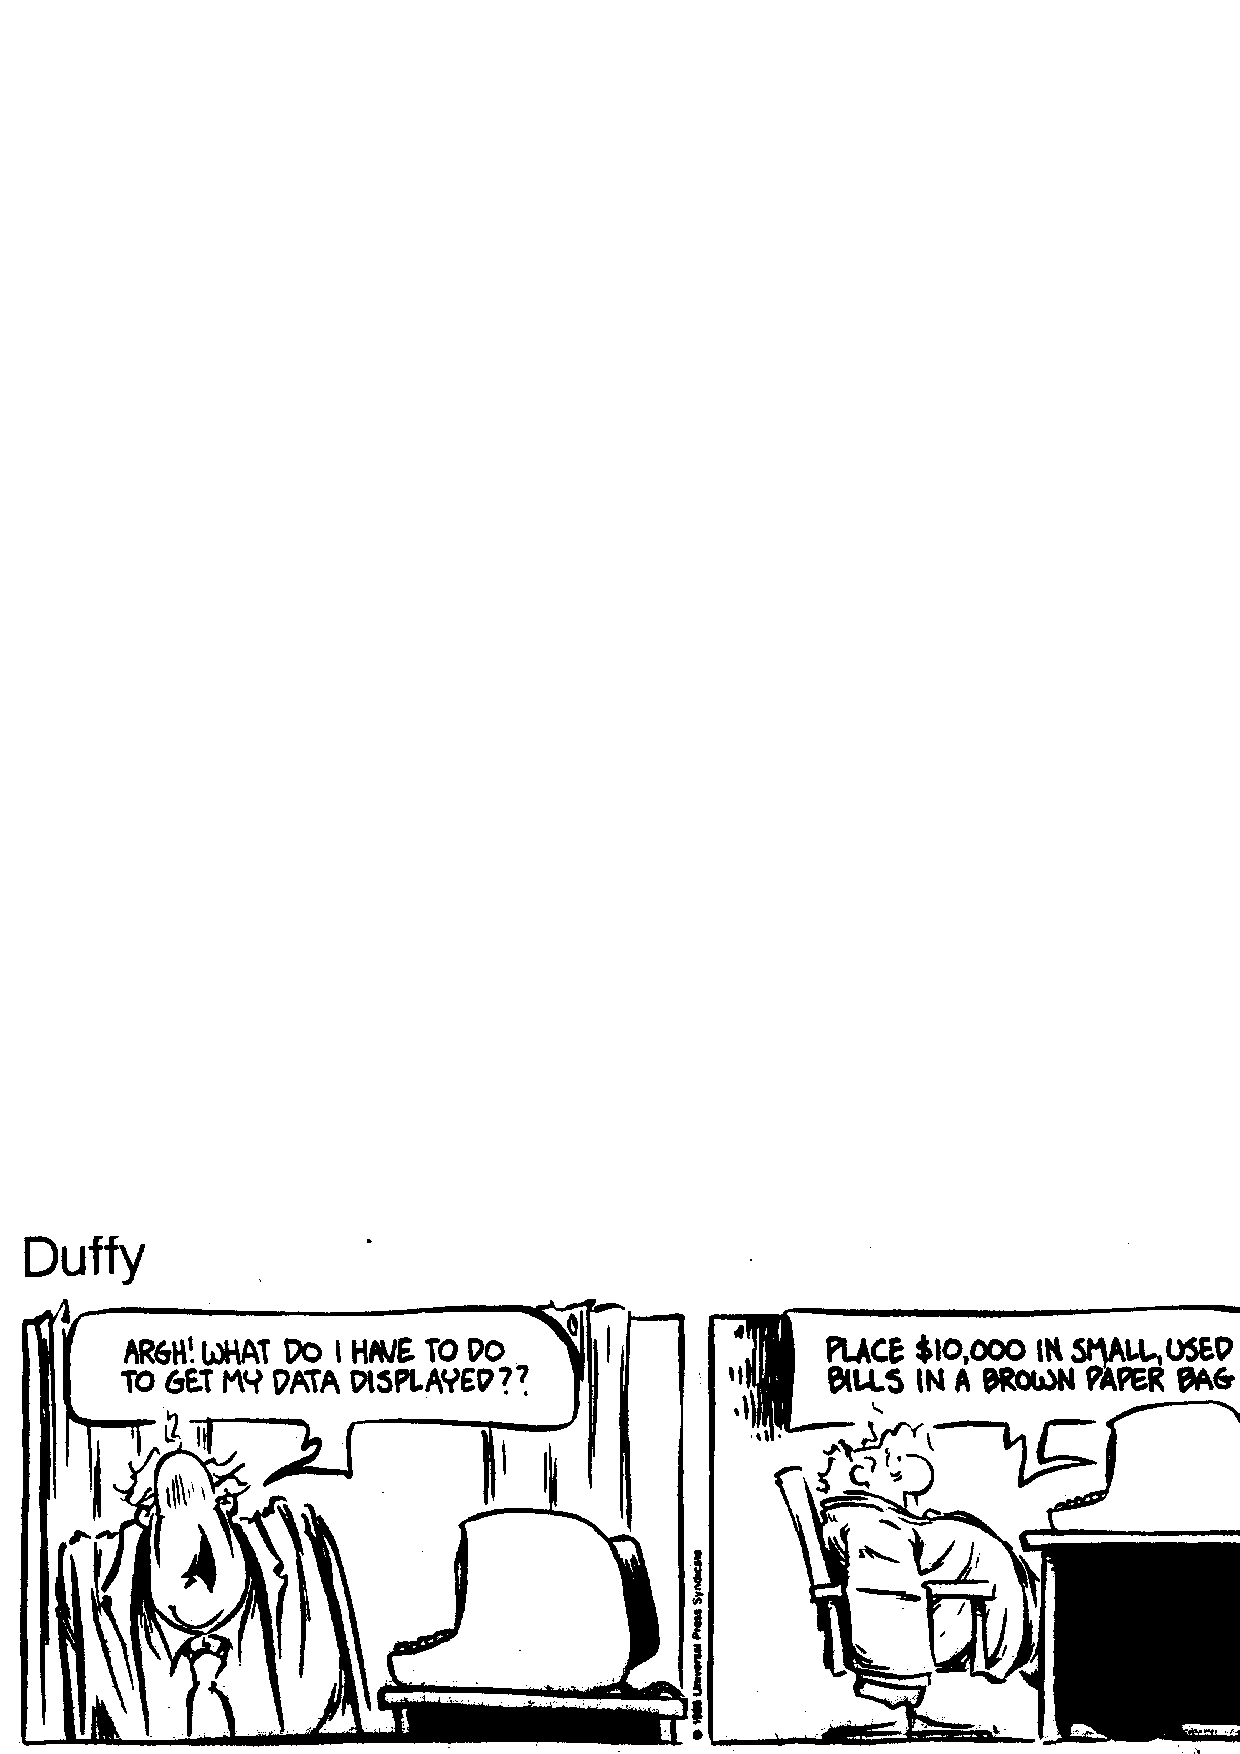
\includegraphics[width=\textwidth]{sc8_duffy}
\caption[Getting plots out]
{\small{Give the bag to your telescope operator}}
\label{fig:duffy}
\end{figure}

\subsection{Getting the data}
\label{sec:getting-the-data}
First read the data with the command \texttt{read-gsd-data}:

\SP\ \texttt{r-g-d}

and \SPECX\ will ask you which data file you want to read with the
following question:

\texttt{GSD scan number? [ ]}

Give it just the relevant part of the scan number.  For example, to
read \texttt{obs\_das\_0030.dat}, one would type the following:

\SP\ \texttt{r-g-d}

and answer the question with \texttt{30}

You could type it all on one line:

\SP\ \texttt{r-g-d 30}

and avoid the dialogue.

In this simple example, I have been at pains illustrate in
considerable detail the character of \SPECX\ commands and the nature
of the dialogue. In most of the following material this level of
detail will be omitted. Generally, \SPECX\ commands are
self-explanatory as a result of the amount of subsidiary verbage.

\begin{aside}
\textbf{How to specify scans observed in groups --- } In many cases, you
will have observed several points in a sequence using the \texttt{GRID},
\texttt{PATTERN} or \texttt{RASTER} observing modes. In such cases, all the
spectra observed in this way are grouped together in a single GSD file
under a single scan number, and each spectrum is also defined by a
sequence number (set by the order in which it was observed) as well as
the scan number.  Thus

\SP\ \texttt{r-g-d 30 4}

will load spectrum sequence number 4 from observation 30.
\end{aside}

Now you want to look at the spectrum.  Just do;

\SP\ \texttt{n}

`{\tt{n}}' stands for `start up \underline{n}ew plot file'; not exactly
obvious, but it makes sense once you are used to it. Actually, it's a
little more subtle than that; the full command is

\SP\ \texttt{new-plot}

and this command requires two variables to be input; pen width and
colour. `{\tt{n}}' alone has been defined as equivalent to
`{\tt{new-plot 1 3}}'.

All this assumes that the plot device is set to `terminal'. If it's not,
and that's the way you want it, first type

\SP\ \texttt{s-p-d t}

before typing \texttt{n} again. If you have turned on the interactive
mode (the default on starting \SPECX \texttt{6.7} for the first time is
non-interactive, an improvement over Version 6.3), then to get out of
the plot hit the `{\tt{e}}' for exit.

A typical spectrum looks like that shown in
Figure~\ref{fig:specx_plot}.
%
\begin{figure}[htb]
\centering
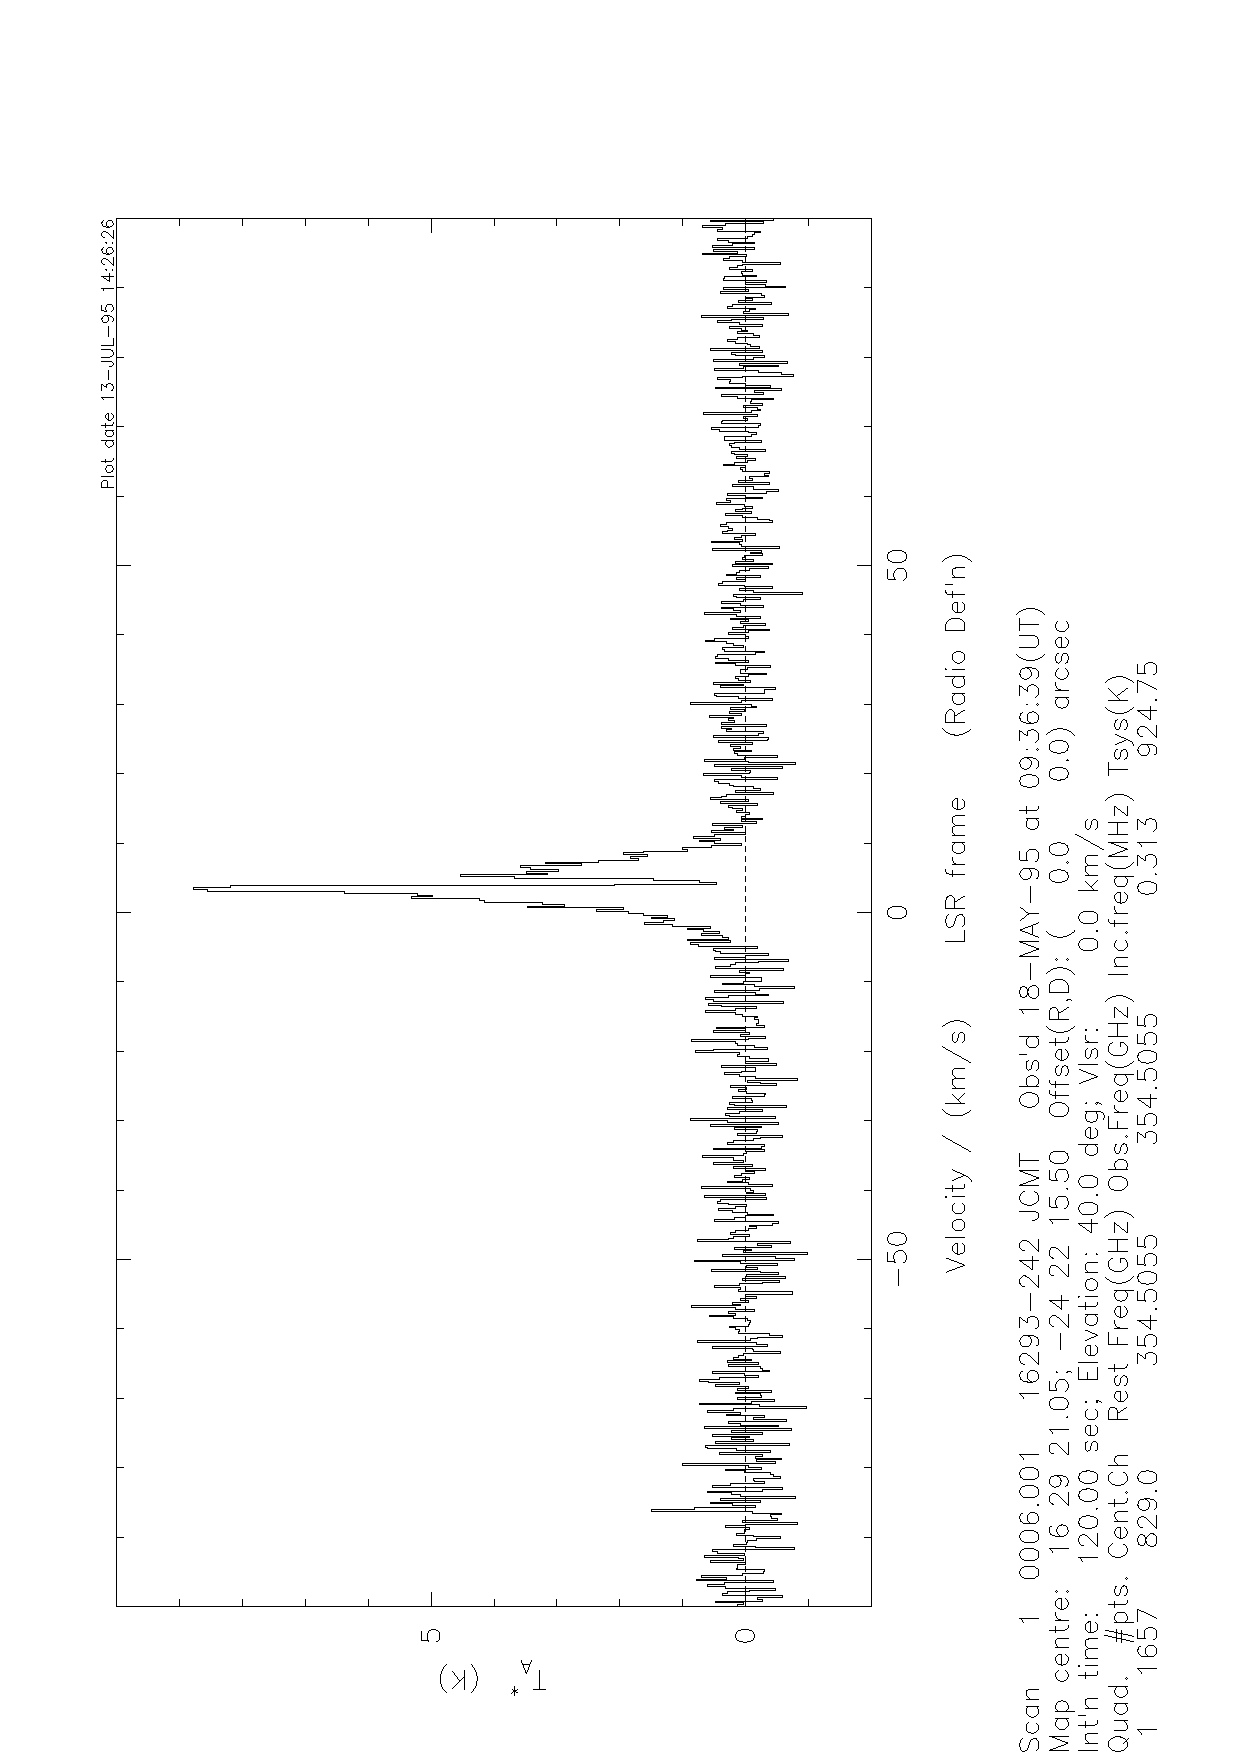
\includegraphics[width=0.8\textwidth]{sc8_spectrum}
\caption[A typical plot]
{\small{A typical spectrum; in this case the scales of the axes have
been set to display the result to good advantage. Below the plot
frame, most of the information which might be needed is present.}  }
\label{fig:specx_plot}
\end{figure}

The spectrum can be plotted in two ways: histogram (the default on
startup), and line (connect the dots). One can also set the line
thickness and the colour (set to 1 and 3 [=green] on startup).
The first two are controlled by the flags
\texttt{histogram} and \texttt{line\_weight}. That is, on startup the
defaults are

\SP\ \texttt{histogram=true}\\
\SP\ \texttt{line\_weight=1}

Typing \texttt{histogram=false} gives a line plot. I wouldn't recommend
using a \texttt{line\_weight} larger than 3. Colour numbers range from 1 to 15.


%\subsection{Things To Do With A Displayed Spectrum}
%\label{sec:specx_5}
\subsubsection{Closing in on your spectrum; interactive \textit{vs}
non-interactive modes}
\label{sec:specx_5.1}
If you are in interactive mode, there are quite a few things
you can do with the spectrum on the screen. The first thing is zoom in
on a small section of it so that you don't have to look at the parts
you can't explain.  There are two ways to do this, both of them easy.

The quick way is to use the mouse cursor (using Xwindows) or the
cross-hairs (if you are working with a VTxxx graphics-compatible
terminal) to make a box around the part you want to look at more
closely. Point the mouse cursor at the position on the Xwindow plot
screen, and type a command. If you're using a VTxxx terminal you use
the arrow keys to move the crosshairs around; holding down the \texttt{Shift} key makes the lines move in large steps.  Place the cursor
position (or intersection of the cross-hairs) on one corner of the box
you want to draw and hit one of the following keys to mark the spot;
\texttt{t}, \texttt{b}, \texttt{l}, \texttt{r}.  For example, to identify the
lower right corner of the box you hit \texttt{b} (for `{\tt{bottom}}') and
\texttt{r} (for `{\tt{right}}'). Now go to the opposite corner and hit the
other two keys (\ie\ \texttt{t} for \texttt{top} and \texttt{l} for \texttt{left}). The box will not appear on the screen until you hit \texttt{d}
for \texttt{draw}.  This will draw the box on the screen. If you made a
mistake drawing the box just try again.  When
you've got the box you want hit \texttt{n} for \texttt{new\_limits} and the
portion of the spectrum inside the box will be replotted.
Table~\ref{tab:specx} (taken from Rachael Padman's \SPECX\ manual
version 6.3) shows other possibilities; I'm sure the options have
increased in number since then, so use the \texttt{h} option (for `help')
to see a complete list.


\begin{table}[htbp]
\begin{center}
\caption{Interactive plotting functions}
\begin{tabular}{|c|l|p{3.7in}|} \hline
Key	& Mnemonic	& Function \\ \hline
H	&HELP	&Produces a list of all valid options\\
?	&QUERY	&Tells you the current coordinates of the cursor\\
L	&LEFT	&Define the left-hand boundary of the current `box'\\
R	&RIGHT	&Define the right-hand boundary of the current box\\
T	&TOP	&Define the top boundary of the current box\\
B	&BOTTOM	&Define the bottom boundary of the current box\\
D	&DRAW	&Draw the current box\\
C	&CLEAR	&Erase the alpha (ASCII) screen\\
Q	&QUIT	&Leave interactive graphics\\
E	&END	&Leave interactive graphics, erase graphics screen\\
N	&NEW\_LIMITS    &
Redraw the plot taking the current box as new
            limits. Note that if the limits have not been
            redefined in one co-ordinate then you get back the
            original limits according to SET-PLOT-SCALES\\
S	&LIMITS	&Lets you set new plot limits by hand\\
A	&ACCEPT	&Tell the program to accept the current box\\
+	&MARK	&Mark position using cross-hair\\
\verb+<CR>+ &RETURN &Accept default box (for input of baseline regions)\\ \hline
\end{tabular}
\label{tab:specx}
\end{center}
\end{table}


If you want exact limits on the axes you can use the second
method. First figure out what the \texttt{x} and \texttt{y} limits are from
your plot. Lets say, for example that you want the \texttt{x} axis to run
from $-50$ to $+50$ km/s and the \texttt{y} axis from $-5$ to 50 Kelvin.
You would use the \texttt{set-plot-scales} command:

\begin{terminalv}
>> set-plot-scales
Do you want automatic scaling of X-axis? (Y/N) [Y] n
X-axis scale: Beginning and end? [ 150.00  300.00] -50 50
Do you want automatic scaling of Y-axis? (Y/N) [Y] n
Y-axis scale: Beginning and end? [ -10.00   10.00] -5 50
..
\end{terminalv}

If you want to see all of the spectrum again then send the following;

\begin{terminalv}
>> s-p-sc
Do you want automatic scaling of X-axis? (Y/N) [N] y
Do you want automatic scaling of Y-axis? (Y/N) [N] y
\end{terminalv}

Note that you can set either of the \texttt{x} and \texttt{y} scales to
automatic scaling, or both. This is a very useful feature.

\subsection{A note on command line syntax}
\label{sec:command-line}
This may be a little tedious by now, so this may be a good time to
introduce the notion of dispensing with the chatter of the
question-and-answer mode.  Once you know what questions \SPECX\ will
ask you can provide the answers before being asked on a \textit{command
line}.  Thus, to set the plot scales above you would type

\SP\ \verb|s-p-sc\n\-50 50\n\-5 50\ |

and to reset the scales to fully automatic

\SP\ \verb|s-p-sc\y\y\ |

Note that the command itself has been shortened to the
minimum-matching level.  If you truncate the command too much \SPECX\
will inform you of all the commands meeting your ambiguous
specification. The backslashes separate command line parameters. They
do not have to be present in this particular case \ie\

\SP\ \verb|s-p-sc y y |

would do. However, it is better to have them there within command
files, especially where a command calls for multiple inputs. Otherwise
the results may be a little strange on occasion.

Parameters may be omitted altogether if you want to take the defaults,
or the previous settings. In this case one can either use the
placeholder symbol
\verb+#+:

\SP\ \verb|s-p-sc\n\#\n\#\ |

or nothing at all:

\SP\ \verb|s-p-sc\\\\\ |

\subsection{Dressing Up Your Spectrum}
\label{sec:specx_5.2}
Now that you've got your spectrum on the screen you can make it look a
little better by doing some simple operations on it.

\subsubsection{Smoothing the data}
\label{sec:specx_binning}
The most common operation is binning over a number of channels.
\SPECX\ asks you how wide the bin should be. It averages the points in
the bin and plots the average.  So if I want to have a bin of width 5 for
the current spectrum I would send the following command:

\begin{terminalv}
>> bin-spectrum
Bin width? (channels) [  3] 5
Data obs'd in LSR  frame; RAD velocity law; Velocity =   -7.000000     km/s
..
\end{terminalv}

A similar operation is smoothing.  \SPECX\ produces a running mean
over the spectrum.  If I want to smooth the current spectrum using a
5-point average the following command will do it.

\begin{terminalv}
>> smooth-spectrum
Running mean over? (points) [ 2] 5
\end{terminalv}

or in a shorter version;

\SP\ \verb|sm-sp 5 |

There are also operations like \texttt{hann-spectrum}, \texttt{convolve-spectrum}, \texttt{fold-spectrum} etc. A comparison of binned
and smoothed spectra is shown in Figure~\ref{fig:specx_smooth}. Note
that the number of channels in the end spectrum is different in each
case. For a DAS spectrum having 1657 channels after merging (see
later), Hanning-smoothing ({\tt{hann}}) reduces that to 1655,
running-mean smoothing over 5 channels ({\tt{sm-sp 5}} gives 1653, and
binning over 5 channels ({\tt{bin 5}}) results in only 331
channels. These differences become \textit{very} important when making
maps. Hanning-smoothing is very effective at removing `ringing' caused
by spikes in the data (cf. Section~\ref{sec:spike-removal}).

\begin{figure}[htb]
\centering
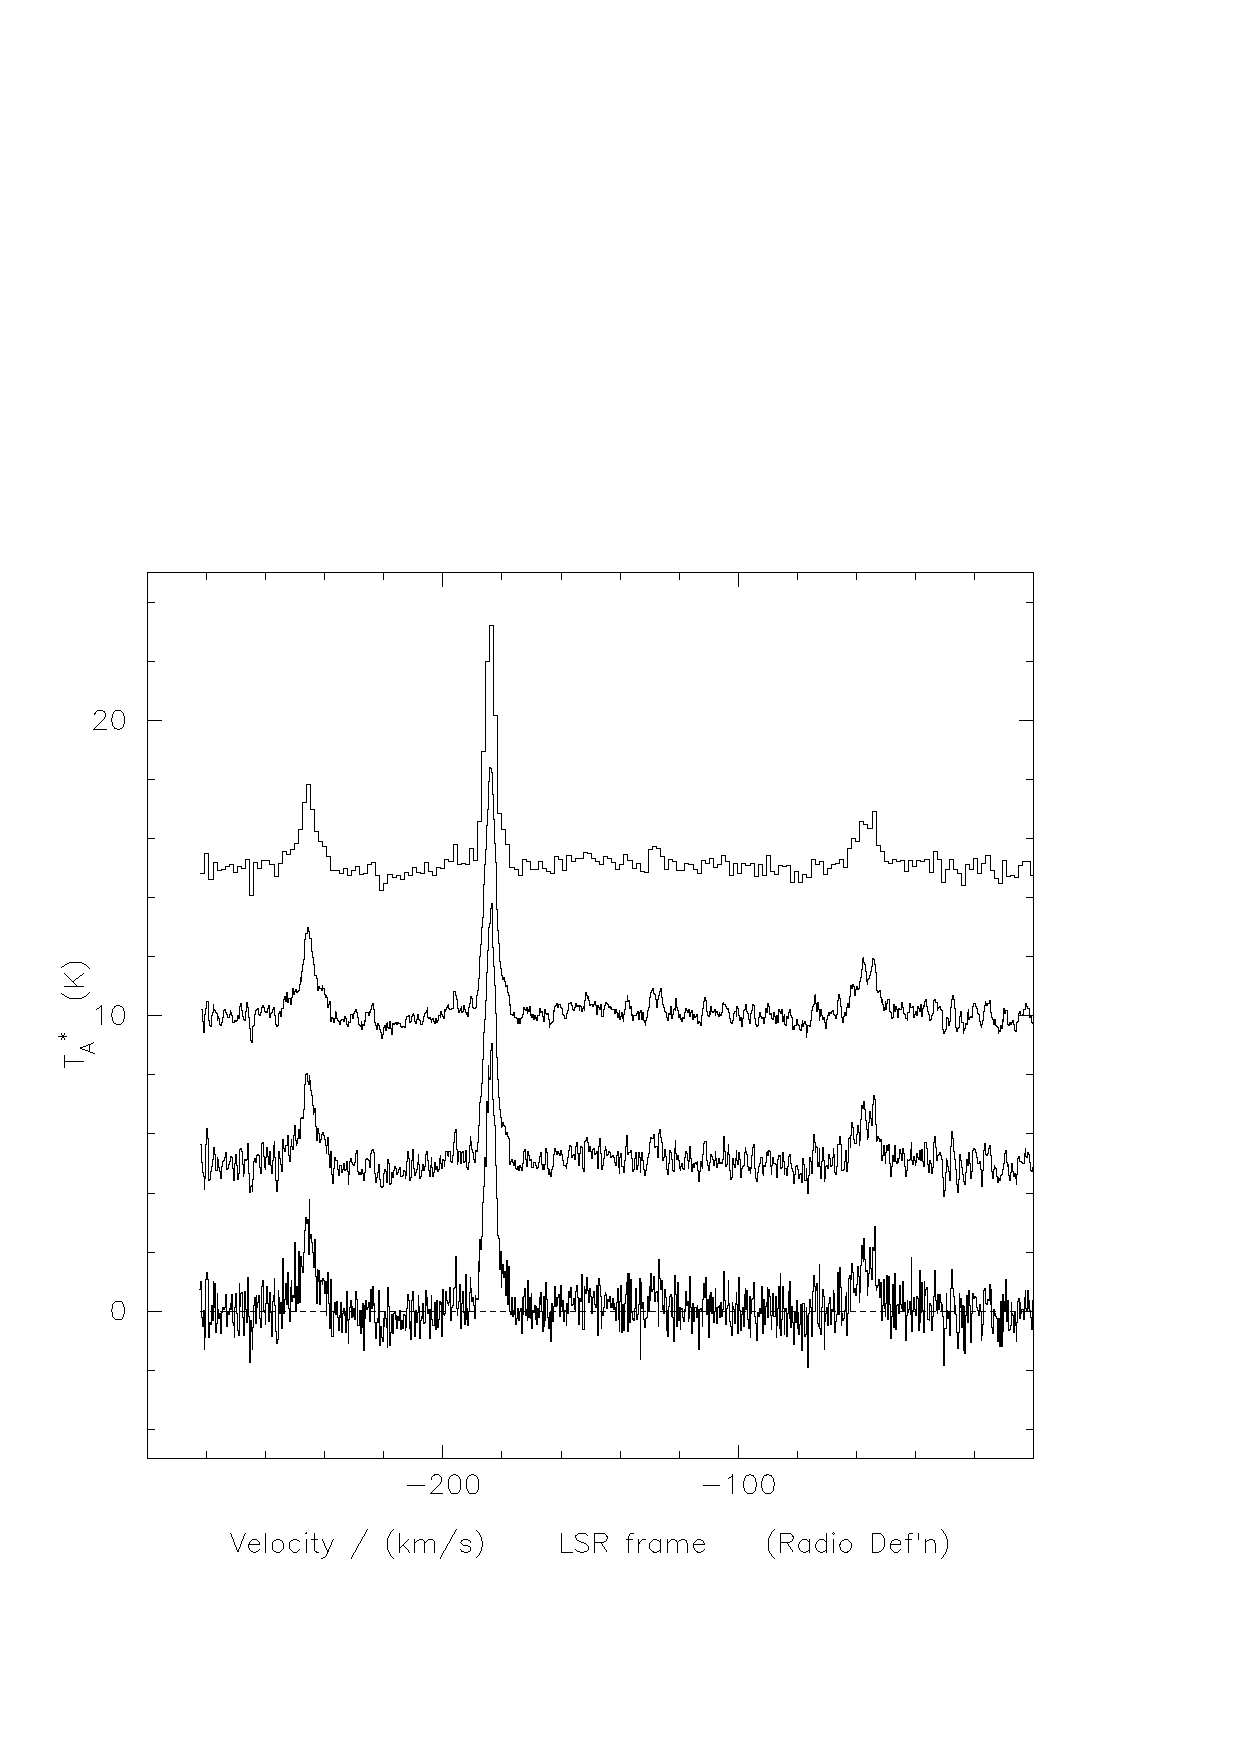
\includegraphics[height=0.8\textwidth]{sc8_smooth}
\caption[Binning and smoothing spectra]
{\small{Using various channel-averaging methods. In order, from bottom
to top, the spectra are (a) the original, (b) Hanning-smoothed (using
\texttt{hann}), (c) smoothed by 5 channels (with \texttt{sm-sp 5}), and (d)
binned over 5 channels (using \texttt{bin 5})} }
\label{fig:specx_smooth}
\end{figure}

\subsubsection{Putting vertical and horizontal lines on the spectrum}
\label{sec:specx_lines}
There are times you may wish to guide the eye of your readers to some
feature of your spectrum. A vertical line (extending the entire height
of the spectrum plot frame) can be put at, say, 56 km/s by typing:

\SP\ \verb|vert 56|

A plot has to be open for this to work. The plot will be redrawn.

In \SPECX\ 6.3 I didn't find any equivalent for horizontal
lines, but if you really want to do
this, one method that works is to multiply your spectrum by zero
number, offset to where you want it vertically, and replot the
spectrum. Thus, say:

\SP\ \verb|mult 0.0; off 2.5; over 1 6|

would put a horizontal line on your open plot 2.5 K above zero. This
also allows one ready control over both line width and color. \SPECX\
6.7 includes the \texttt{baseline} command which implements this sequence
for you.

\subsection{Getting To Know Your Baselines}
\label{sec:specx_5.3}
If you want to start a little data reduction on your spectrum you can
remove some baselines or fit some models.  There seems to be some
controversy about the names of the commands though.  Some people claim
that a gaussian is not a baseline, it's a model. The difference lies
in whether one is removing an instrumental `baseline' or curve which
underlies the line itself, or whether one is fitting the line itself
with a `model'.

When fitting baselines or models, or doing a number of other
operations on spectra, one or more sections of the spectrum need to be
specified. For a linear baseline fit, \emph{two} regions of the baseline need
to be identified for the fit. In the case of polynomial fits, one to
several such regions can be specified. And for a gaussian fit, one
specifies not the baseline, but the line region to be fit. It all
makes sense really. Just try it.

One can specify the fit regions either in interactive mode, in which
case the cursor (or crosshair) is used to define sections of the
spectrum, or by specifying the same sections by typing in the numbers
in non-interactive mode.  In my view interactive mode can be a pain to
use, but the results are worth it. The procedures outlined next for
fitting a linear baseline will apply to all situations where x-value
ranges are called for.

\subsubsection{Linear baselines}
\label{sec:linear-baselines}
To take a linear baseline out of your spectrum use the command \texttt{remove-linear-baseline}.  For example, I want to remove a linear
baseline from the current spectrum.  The following command will do
it:

\SP\ \verb|r-l-b|

If you are in \textit{interactive mode} the screen will display the current
spectrum with the first of the previously chosen boxes (if any)
outlined in dot-dashed lines. \textit{If you are using Xwindows click
first on the title bar at the top of the plot window} -- it will be
labelled ``{\tt{PGPLOT Window 1}}''; depending on how your system is
set up clicking elsewhere in the window may give erroneous results.
Then either
\begin{itemize}
\item
tap the return key at this point to choose the range shown (which will
then be displayed in solid lines), and display the second range. You
have the option of taking this one too, in which case you are finished
with this fit.
\item
or, alternatively, move the cursor or cross-hair to a somewhat flat
part of the noise to the left of the spectral line and hit `{\tt{l}}'
(for `{\tt{left}}') and then move a little to the right (still to the
left of the spectral line) and hit `{\tt{r}}' (for `{\tt{right}}') and
finally `{\tt{a}}' (for `{\tt{accept}}').  Now a box will appear on the
screen corresponding to the range between the chosen \texttt{l} and \texttt{r} positions.  Now go to the right side of the spectral line and do
the same thing.  When you hit `{\tt{a}}' this time though, the baseline
will have been subtracted and the end result will be in the current
spectrum buffer.
\end{itemize}
To see the end result, all you need to do now is type `{\tt{n}}'.
Remember, to get out of the interactive mode, type `{\tt{e}}' with the
cursor anywhere inside the plot window. If you want to leave the
interactive mode altogther use the command

\SP\ \verb|s-i n|

In non-interactive mode the following exchange is typical. The result
in this particular instance is shown in
Figure~\ref{fig:specx_rlb}. Remember, \texttt{EOF} is \ctrld .
\begin{terminalv}
 >> r-l-b
 Doing R-L-B for quadrant/sub-band #   1
   2 baseline regions currently defined
  Type intervals, one at a time, EOF to finish
 Current units are km/s

 # [   46.00,   56.03] 30 50
 # [   80.00,   90.02] 80 100
 >>
\end{terminalv}
%
\begin{figure}[htb]
\centering
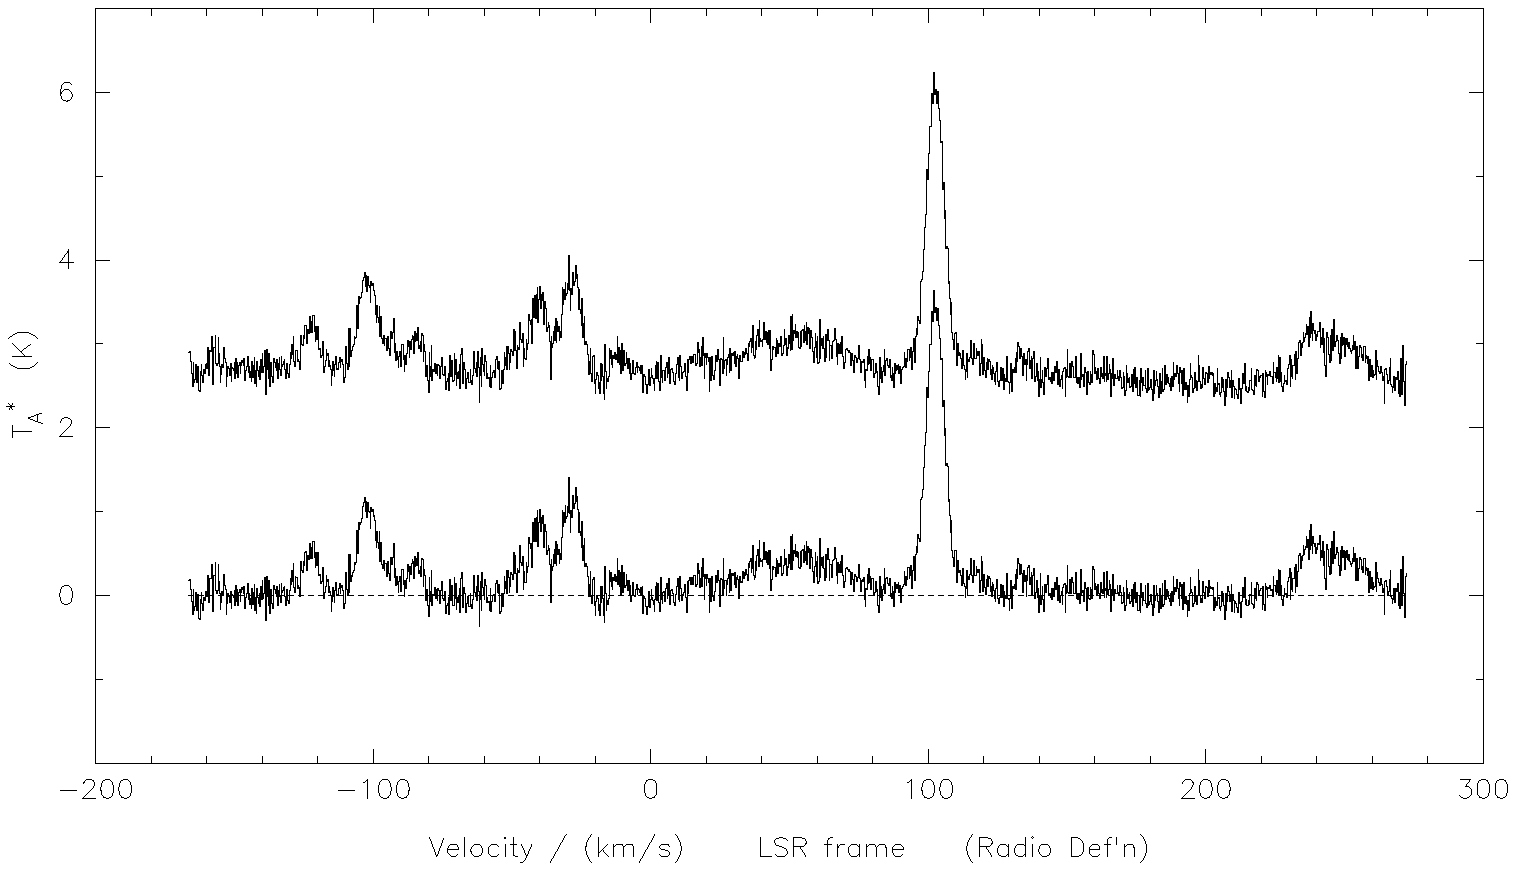
\includegraphics[width=0.8\textwidth]{sc8_rlb}
\caption[Removing a linear baseline]
{\small{The upper spectrum is the original after averaging several
observations. Basically in this case there is an offset in the
baselevel due to the continuum background of the source (G34.3). Below
it is the effect of removing a linear baseline tied to clean
(line-free) regions of the spectrum.}  }
\label{fig:specx_rlb}
\end{figure}

\subsubsection{Polynomial baselines}
\label{sec:poly-baselines}
Fitting a polynomial baseline is similar, by using the command

\SP\ \verb|fit-polynomial-baseline|

\texttt{f-p-b} will do. A typical bad baseline requiring a polynomial fit
is shown below in Figure~\ref{fig:specx_badbaseline}.

\begin{figure}[htb]
\centering
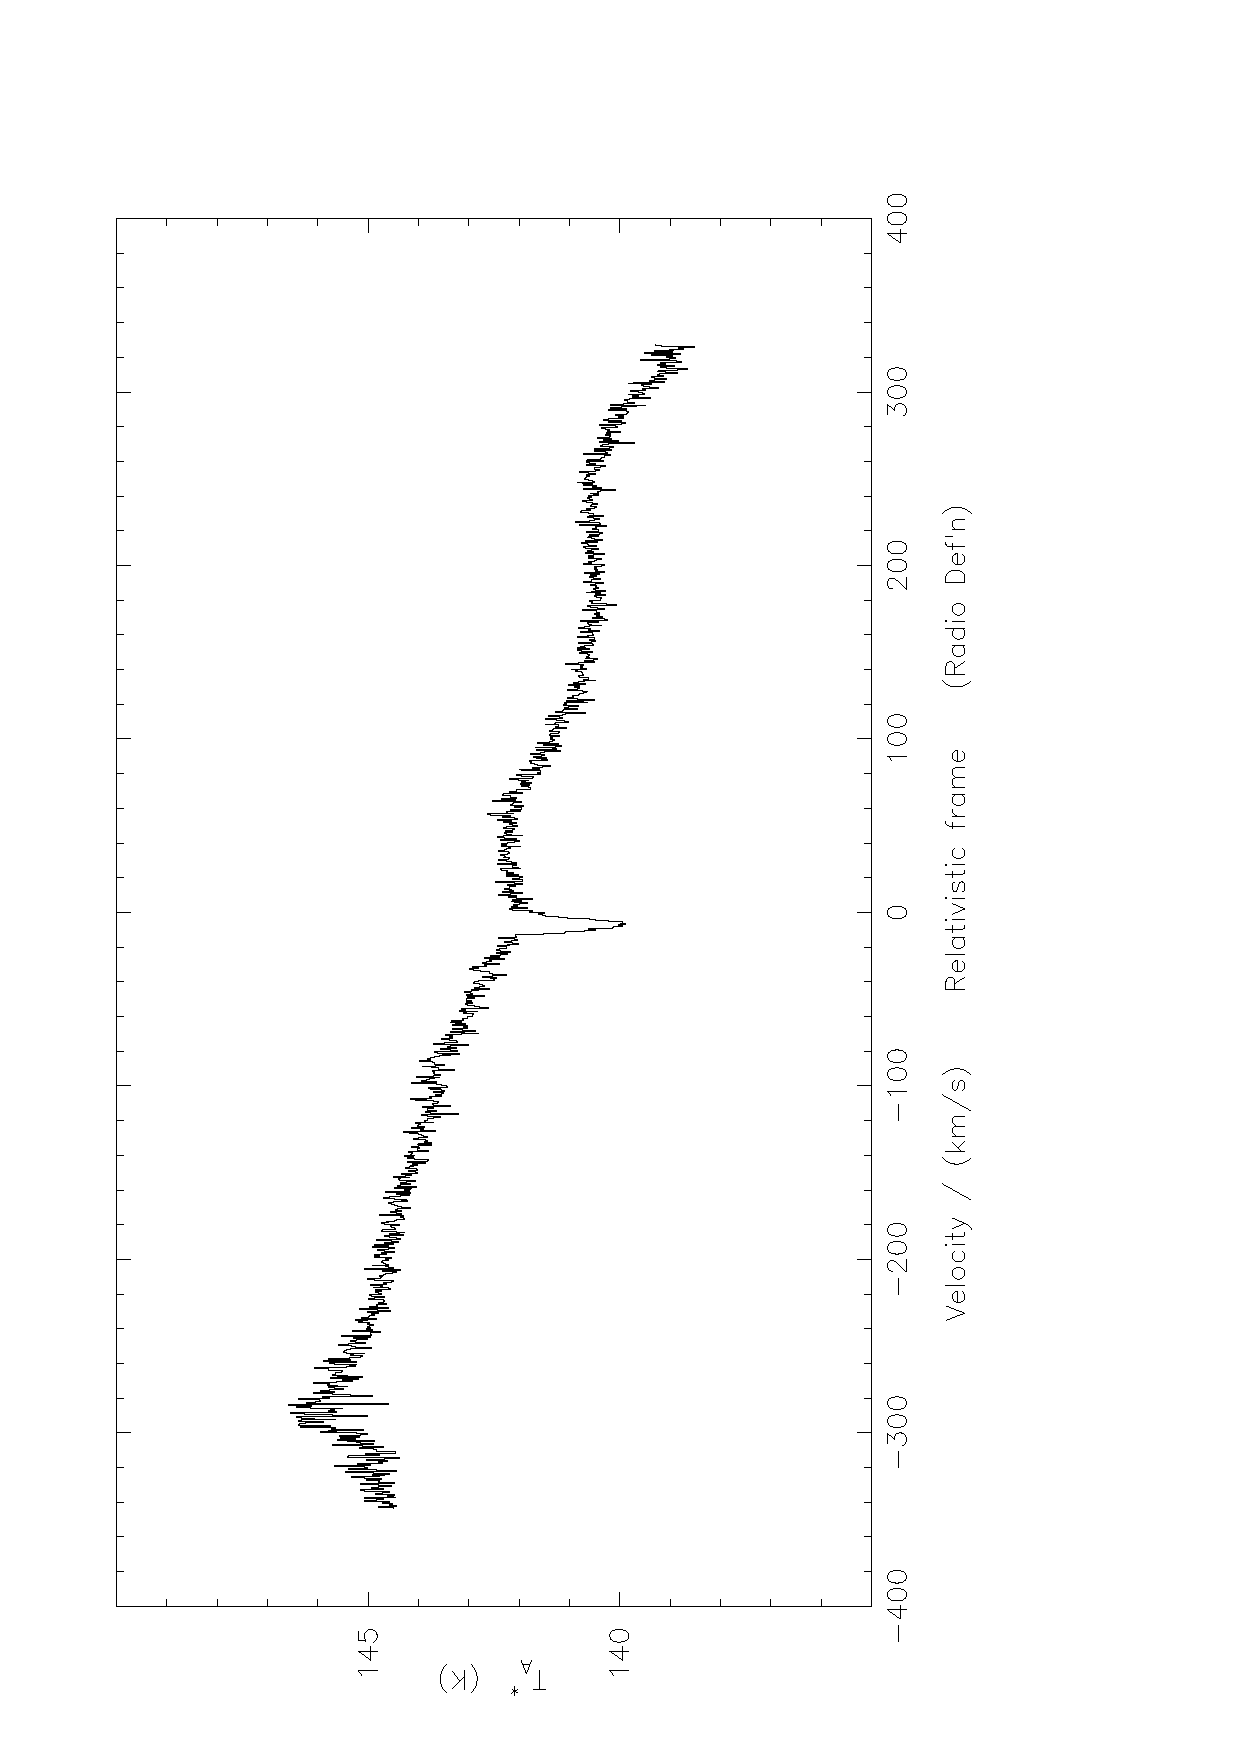
\includegraphics[width=0.8\textwidth]{sc8_badbaseline}
\caption[Typical bad baseline]
{\small{This spectrum was obtained towards a bright planet. The
penalty is the poor baseline, even though beam-switching in azimuth
was used.  }}
\label{fig:specx_badbaseline}
\end{figure}

Again, in interactive mode the screen will display the current
spectrum and you have to tell it where to fit the polynomial.  There
are two differences from a linear baseline removal though; first, you
can choose \textit{one or more} regions, and second, after you fit a
baseline \SPECX\
won't remove it until you tell it to.  You use the same keys as
before, \texttt{l} for the left boundary of a region, \texttt{r} for the
right and \texttt{a } to accept the region. When you are done marking
regions, hit the \texttt{e} for exit and \SPECX\ will ask you for the
order of polynomial you want and then make its fit.

In non-interactive mode the exchange might look like:
\begin{terminalv}

 >> f-p-b
   4 baseline regions currently defined
  Type intervals, one at a time, EOF to finish
 Current units are km/s

 # [  -15.96,   10.59] 0 20
 # [   26.37,   40.18] 30 60
 # [   47.76,   56.77] 80 100
 # [   85.82,  105.52]
 Order of polynomial to be fitted? [ 5] 4
 >>
\end{terminalv}

The fitted baseline is now the current spectrum in the x-register, so if
you want to
look at it just use the \texttt{overlay} command; \eg :

\SP\ \verb|over 1 5|

As shown in Figure~\ref{fig:specx_fpb} this will plot the fitted curve
on top of the original spectrum.

\begin{figure}[htb]
\centering
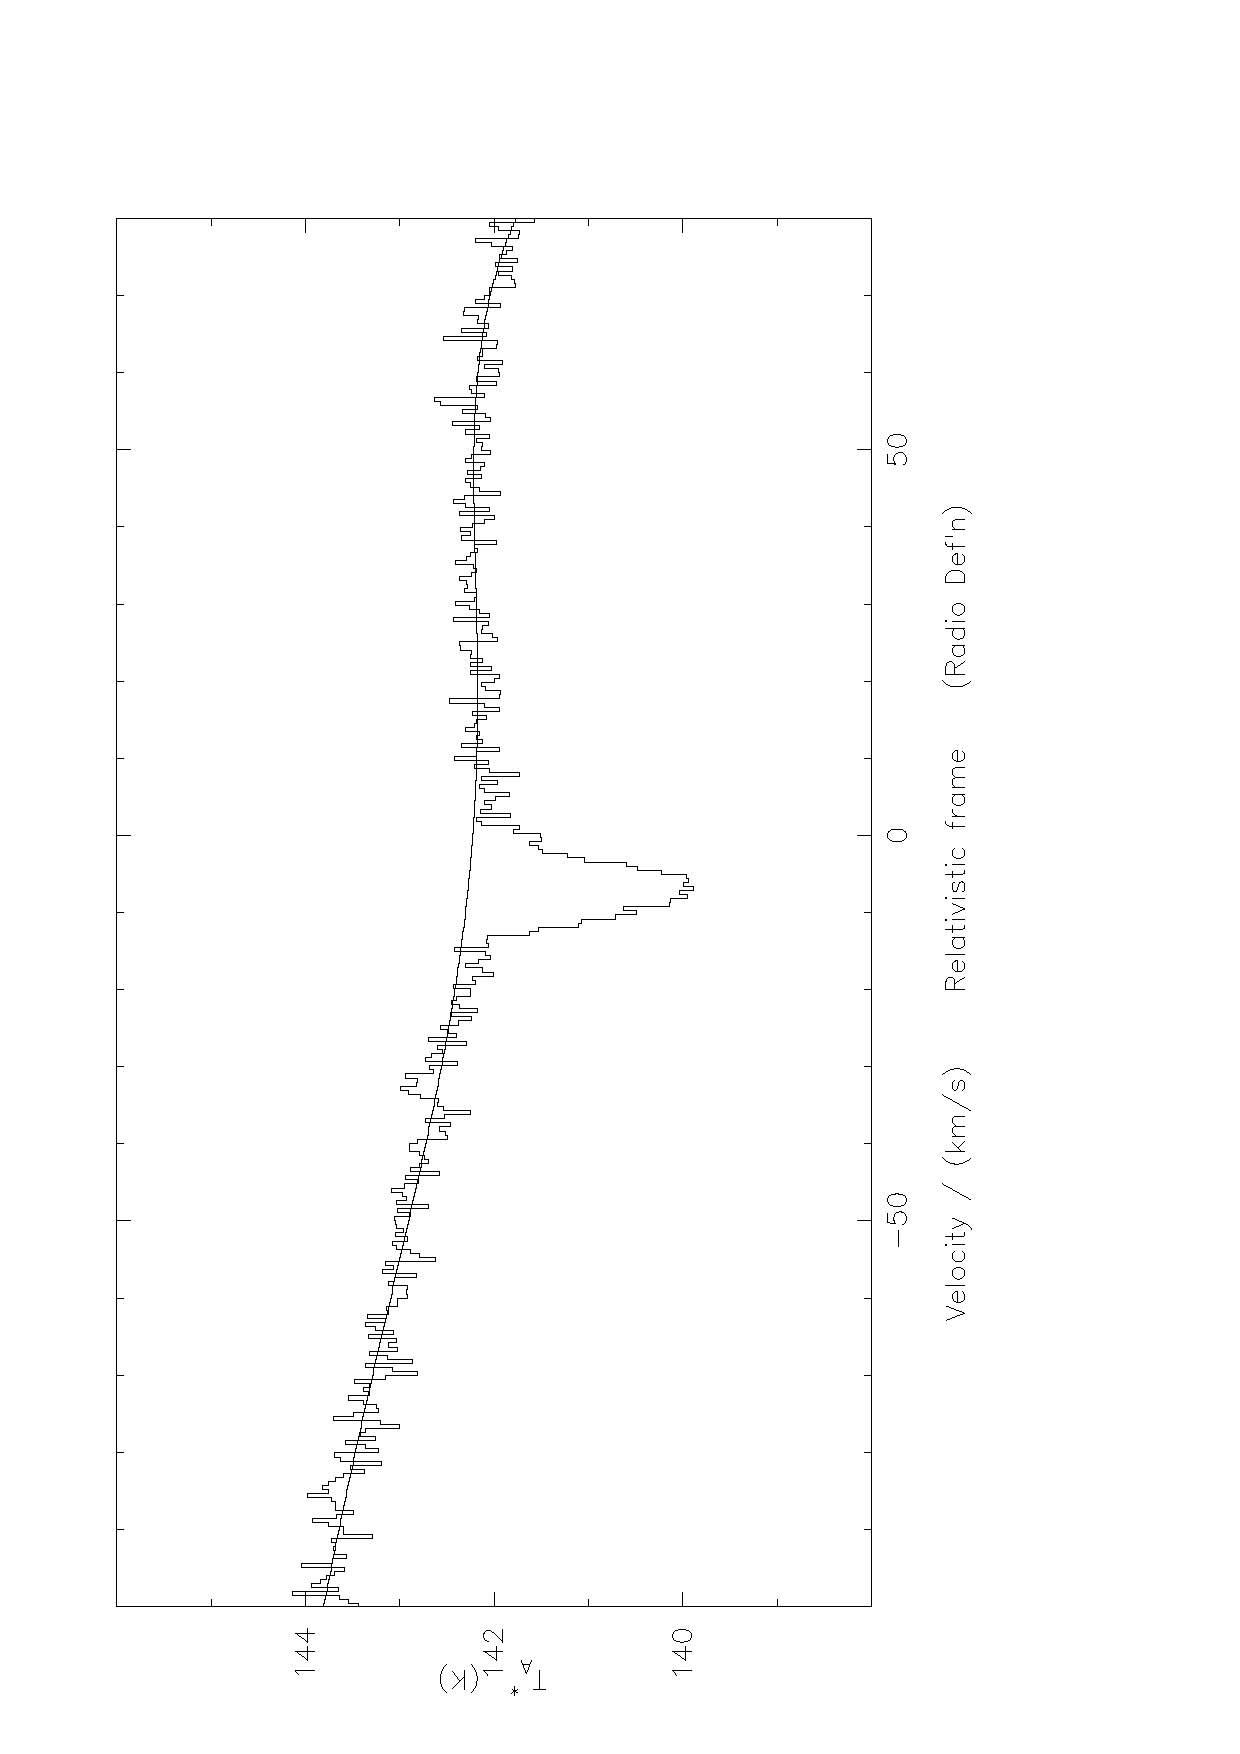
\includegraphics[width=0.8\textwidth]{sc8_fpb}
\caption[A polynomial baseline fit]
{\small{A portion of the baseline of the spectrum in
Figure~\ref{fig:specx_badbaseline} fitted with a polynomial function
using \texttt{f-p-b}. The polynomial has been overlaid on the original
spectrum.  }}
\label{fig:specx_fpb}
\end{figure}

To remove the baseline from the spectrum you subtract the fit from the
original (this places the difference in the top buffer): \ie\ to
subtract the fit and display the result type

\SP\ \verb|sub;n|

In the cases of complex baselines in which you see baseline ripple
(\ie\ sinusoidal effects) using the command \texttt{fit-composite-baseline} ({\tt{f-c-b}}) can be a better choice. However,
it is necessary to experiment with this command to achieve the best
results.

\subsubsection{Gaussian models}
Gaussian fitting is done in a similar way.  The only difference is
that here you need to \textit{specify the line region, rather than outside
it}. You will be asked for initial guesses for the amplitude, width and
position of each gaussian you want to fit. A helpful hint here is to
make use of the ability of \SPECX\ to write output (such as Guassian
fit parameters) to a file. To do this type

\SP\ \verb|s-l-f f| \textit{file-name}

where \textit{file-name} is your choice of file to which to write the
information.  Remember to reset the output to your screen subsequently
(use \texttt{s-l-f t}).

The key commands here are \texttt{fit-gaussian-model} and \texttt{calculate-gaussian-model}, \texttt{f-g-m} and \texttt{c-g-m} respectively.

In non-interactive mode, the dialog might proceed as follows:
\begin{terminalv}
>> f-g-m

          1 baseline regions currently defined
Type intervals, one at a time, EOF to finish
Current units are km/s

# [  -30.15,   10.02] -30 15
#  Exit

Estimates of Amp.,Width(FWHM) and Pos'n for each line
Line at a time, EOF to finish

Current units are km/s

Line  1: [  -2.4  8.7    -7.0] -2.2 9. -8
Line  2: -0.3 25 -8
Line  3:  Exit

         No of Iterations =     4          Final SUMSQ = 0.1725E+01

                  Parameters of current gaussian model

                 N       Amp.        Width (km/s)    Pos'n (km/s)
                 1     -2.152           7.66            -7.04
                 2     -0.277          22.02            -4.64

Baseline calculated - Pushed into stack
..

>> c-g-m
Unknown velocity frame: R
Line or range of lines to model? (EOF to finish) [ 1, 1] 1,2
Line or range of lines to model? (EOF to finish) [ 1, 2]  Exit
\end{terminalv}

What happened here was I used \texttt{f-g-m} to fit the velocity range
surrounding with two Guassian components as specified. Then I used
\texttt{c-g-m} to calculate the curve corresponding to these components
(which is placed at the top of the stack) and then plotted it on the
same axes as for the spectrum.  The result of this is shown in
Figure~\ref{fig:specx_fgm}.

\begin{figure}[htb]
\centering
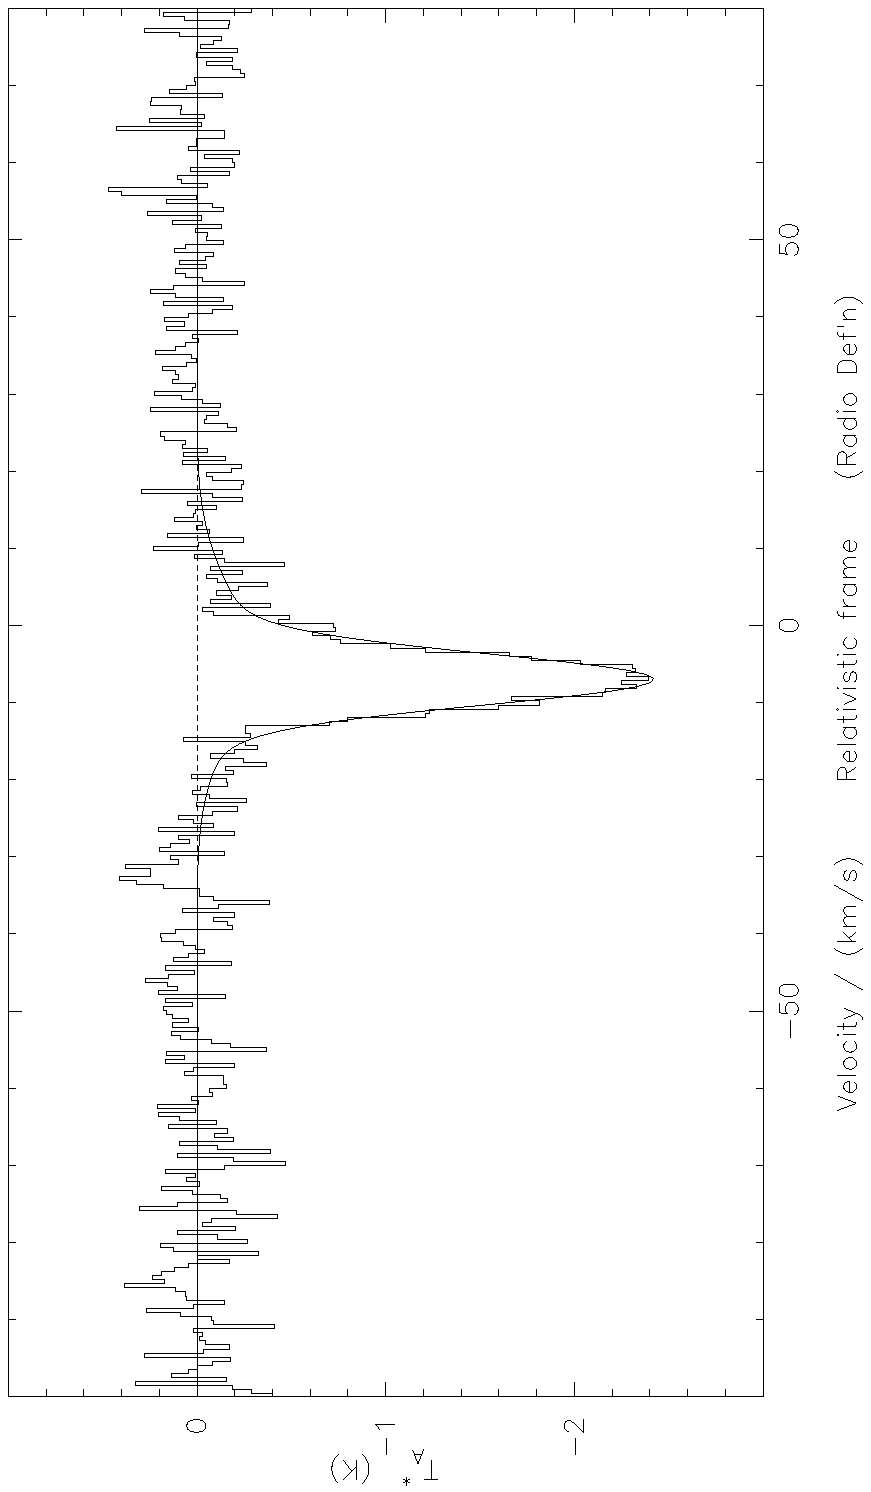
\includegraphics[width=0.8\textwidth]{sc8_cgm}
\caption[A gaussian model fit]
{\small{The spectrum in Figure~\ref{fig:specx_fpb} after subtraction
of a polynomial baseline, showing a fit, plotted as a continuous line
by using \texttt{histogram=false}, of two gaussian components as given in
the example in the text. Fitting two gaussians may be a little
misleading here, since the broader, weaker component could be a
baseline artifact, or could result from pressure broadening of the
line. In the latter case a Voigt profile should be a better fit.  }}
\label{fig:specx_fgm}
\end{figure}

\subsection{The Stack}
\label{sec:specx_6}
We have alluded a couple of times to the presence of internal arrays
in which data is stored once in a while. Now is the time to formalize
that knowledge.
\SPECX\ uses a `stack' to keep spectra in order.  The stack is modeled after
the Hewlett-Packard calculator reverse Polish logic, which some people
seem to have trouble with.

Most of the time all you have to remember is that the current spectrum
(the one that gets plotted with the \texttt{n} command) is in the
x-register. This may (in the case of \texttt{f-p-b}) be a fitted
baseline. If you load one spectrum and then another, the first is
pushed down into the y-register, and the second goes into the
x-register. The command \texttt{ave} averages the two, and places the
result into the x-register. This is all carefully described in the
\SPECX\ manual. However, in case you need to understand more (that is,
you happen to be a Luddite who likes the typical department-store
calculator better than an HP), you can see the contents of the stack
using the command

\SP\ \verb|show-stack|

For department-store calculator people it's important to know that
\emph{the stack is upside-down}. Position X is the bottom and T is the
top.  The spectrum in the bottom register is the current one.

There are four operations you can do to move the stack registers
around and one command to clear the stack which is, of course, \texttt{clear-stack}. The four operations are; \texttt{xy-interchange}, \texttt{roll-stack}, \texttt{push-stack-up}, and \texttt{pop-stack-down}. \texttt{xy},
\texttt{roll}, \texttt{push} and \texttt{pop} will suffice.

Table~\ref{tab:specx_tab1} shows the results of these four commands.

\begin{table}[htb]
\caption{Understanding stack operations}
\begin{center}
\begin{tabular}{ccccc}
Stack posn & Scan no &      & Stack posn & Scan no \\
X & 001 &                                & X & 002 \\
Y & 002 & {\huge $\Longrightarrow$}      & Y & 001 \\
Z & 003 & {\footnotesize XY-INTERCHANGE} & Z & 003 \\
T & 004 &                                & T & 004 \\
  &     &                                &   &     \\
X & 001 &                                & X & 002 \\
Y & 002 & {\huge $\Longrightarrow$}      & Y & 003 \\
Z & 003 & {\footnotesize ROLL-STACK}     & Z & 004 \\
T & 004 &                                & T & 001 \\
  &     &                                &   &     \\
X & 001 &                                & X & 001 \\
Y & 002 & {\huge $\Longrightarrow$}      & Y & 001 \\
Z & 003 & {\footnotesize PUSH-STACK-UP}  & Z & 002 \\
T & 004 &                                & T & 003 \\
  &     &                                &   &     \\
X & 001 &                                & X & 002 \\
Y & 002 & {\huge $\Longrightarrow$}      & Y & 003 \\
Z & 003 & {\footnotesize POP-STACK-DOWN} & Z & 004 \\
T & 004 &                                & T &     \\
\end{tabular}
\label{tab:specx_tab1}
\end{center}
\end{table}

\subsection{Saving Reduced Data for later}
\label{sec:specx_7}
\subsubsection{Using Data Files}
\label{sec:data-files}
As you can see, the stack is not a good place to keep a spectrum after
you have spent time removing baselines and smoothing it.  It can
easily get lost in the shuffle of the stack.  The safe place to keep a
polished spectrum is in its own special file which you can close and
re-open later when you have time.

A single file can contain any number of spectra.  First you have to
open a file with the \texttt{open-file} command.  Then \SPECX\ will ask
you what you want to call the file, and a couple of other questions.

Lets say I have just removed a baseline from my spectrum and now I
want to save it for later.  For now I only want the one spectrum in the
file, but I can put more in the file later; the file is in principle
infinitely expandable. The name of the file will be \texttt{stanley}
(under Unix the file will be called \texttt{stanley.sdf}; the filetype
\texttt{.sdf} is the default). Here is the command dialog:

\begin{terminalv}
 >> open-file
 File name? stanley
 Data file stanley does not exist.
 Create a new file? (Y/N) [N] y
 File title? My_data
 File owner? TMW
 >>
\end{terminalv}

The answers to the questions about file title and owner are not crucial.
They will only appear if you make a listing of the file contents. However,
\textit{do not allow spaces, dashes, or semicolons} to appear in either
field, or, for that matter, in the filename; otherwise the results will
not be what you wanted.

Now a file \texttt{stanley.sdf} will appear in my directory.  To get the
data into the file you use \texttt{write-spectrum}.  This puts the
spectrum in the stack X register into the file.  So I do the following
command;

\begin{terminalv}
 >> write-spectrum
 File number? (EOF to list) 1
 Filed as scan   1 of stanley
 >>
\end{terminalv}

When first created the file access is set to write-only. When opened on
subsequent occasions the default file access is read-only. If you want to
change this use the \texttt{set-file-access} command:

\begin{terminalv}
>> set-file-access
File number? (EOF to list) 1
File access ? (R/W/RW) rw
\end{terminalv}

To close a file use \texttt{close-file}.  You can have up to eight files open
at any one time.  If you want to see which files are open, and what their
access rights are, do;

\begin{terminalv}
>> list-open-files
1  s140_a2_ave                               RW  -1
2  hhhs                                      RW  -1
3  stanley                                   R   -1
\end{terminalv}

To retrieve a spectrum from a file you use the command \texttt{read-spectrum}.  The file you want to read has to be open and have
read access: \eg

\begin{terminalv}
>> rea-sp
File number? (EOF to list) [1]
Scan? 2
>>
\end{terminalv}

\subsubsection{Temporary Storage}
\label{sec:temp-storage}
Several storage registers are available to allow intermediate results,
such as a partial average, to be stored temporarily. To store the
contents of the stack X-register in storage register 2, type:

\SP\ \texttt{sto-sp 2}

To retrieve it at a later time, type:

\SP\ \texttt{reca-sp 2}


\subsection{Using \texttt{das-merge}}
\label{sec:das-merge}
For observations using the DAS it is necessary to remember that for
all but the narrowest bandwidth (125 MHz) the spectrum obtained
consists of 2, 4, or 8 subbands. As noted elsewhere, these subbands
are contiguous in channel space, but overlap in frequency/velocity
space. Each subband has edge effects which should be removed before
gluing the spectrum together. The function \dm\ uses a specified
number of overlap channels from the ends of each subband to average
the overlap regions, optionally with vertical realignment of the
subbands.

\subsubsection{The Principles}
If one were to plot a spectrum before using \dm\ one would obtain
something like the spectrum in Figure~\ref{fig:dm_dirty}.
%
\begin{figure}[htb]
\centering
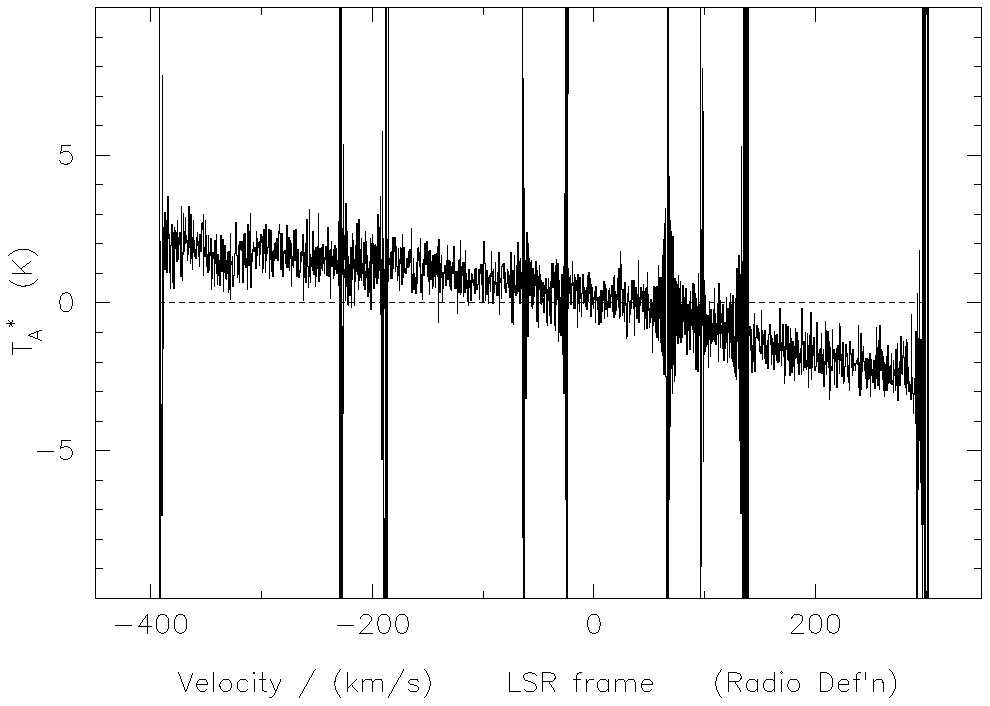
\includegraphics[width=0.8\textwidth]{sc8_dm_dirty}
\caption[Spectrum without \dm ]
{\small{A spectrum consisting of 4 subbands (500 MHz total bandwidth)
taken with a very short integration with receiver A2, plotted without
applying \dm .  The edge effects of the overlapping subbands appear as
sharp spikes; one spike, at 70~km/s is however due to interference
within the bandpass.}}
\label{fig:dm_dirty}
\end{figure}

For illustration purposes, if we stagger the subbands vertically
using the \texttt{set-quadrant-display} and \texttt{offset} commands in
tandem, then the overlap between subbands becomes clear, as in
Fig.~\ref{fig:before-das-merge}.

\begin{figure}[ht]
\centering
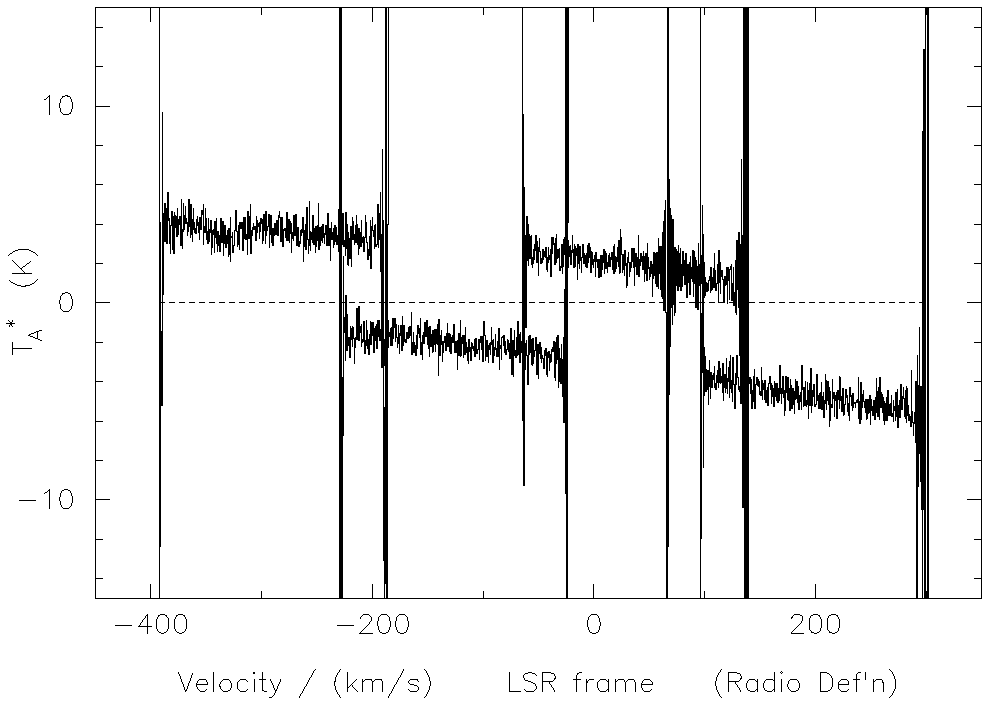
\includegraphics[width=0.8\textwidth]{sc8_dm_orig}
\caption[Before \texttt{das-merge}]
{\small{The spectrum before applying \texttt{das-merge}. Quadrants are
offset from each other for clarity.
}}
\label{fig:before-das-merge}
\end{figure}

\dm\ in fact combines two commands. First it strips off the spiky ends of each
subband, using the \texttt{drop-channels} command. The best number of
channels dropped from each end of each subband depends on the
bandwidth to some extent, but is typically 15--30. The default is set
to half the subband overlap. Using the same staggered subband display
for clarity the end result looks like that in Fig.~\ref{fig:after-das-merge}.

\begin{figure}[ht]
\centering
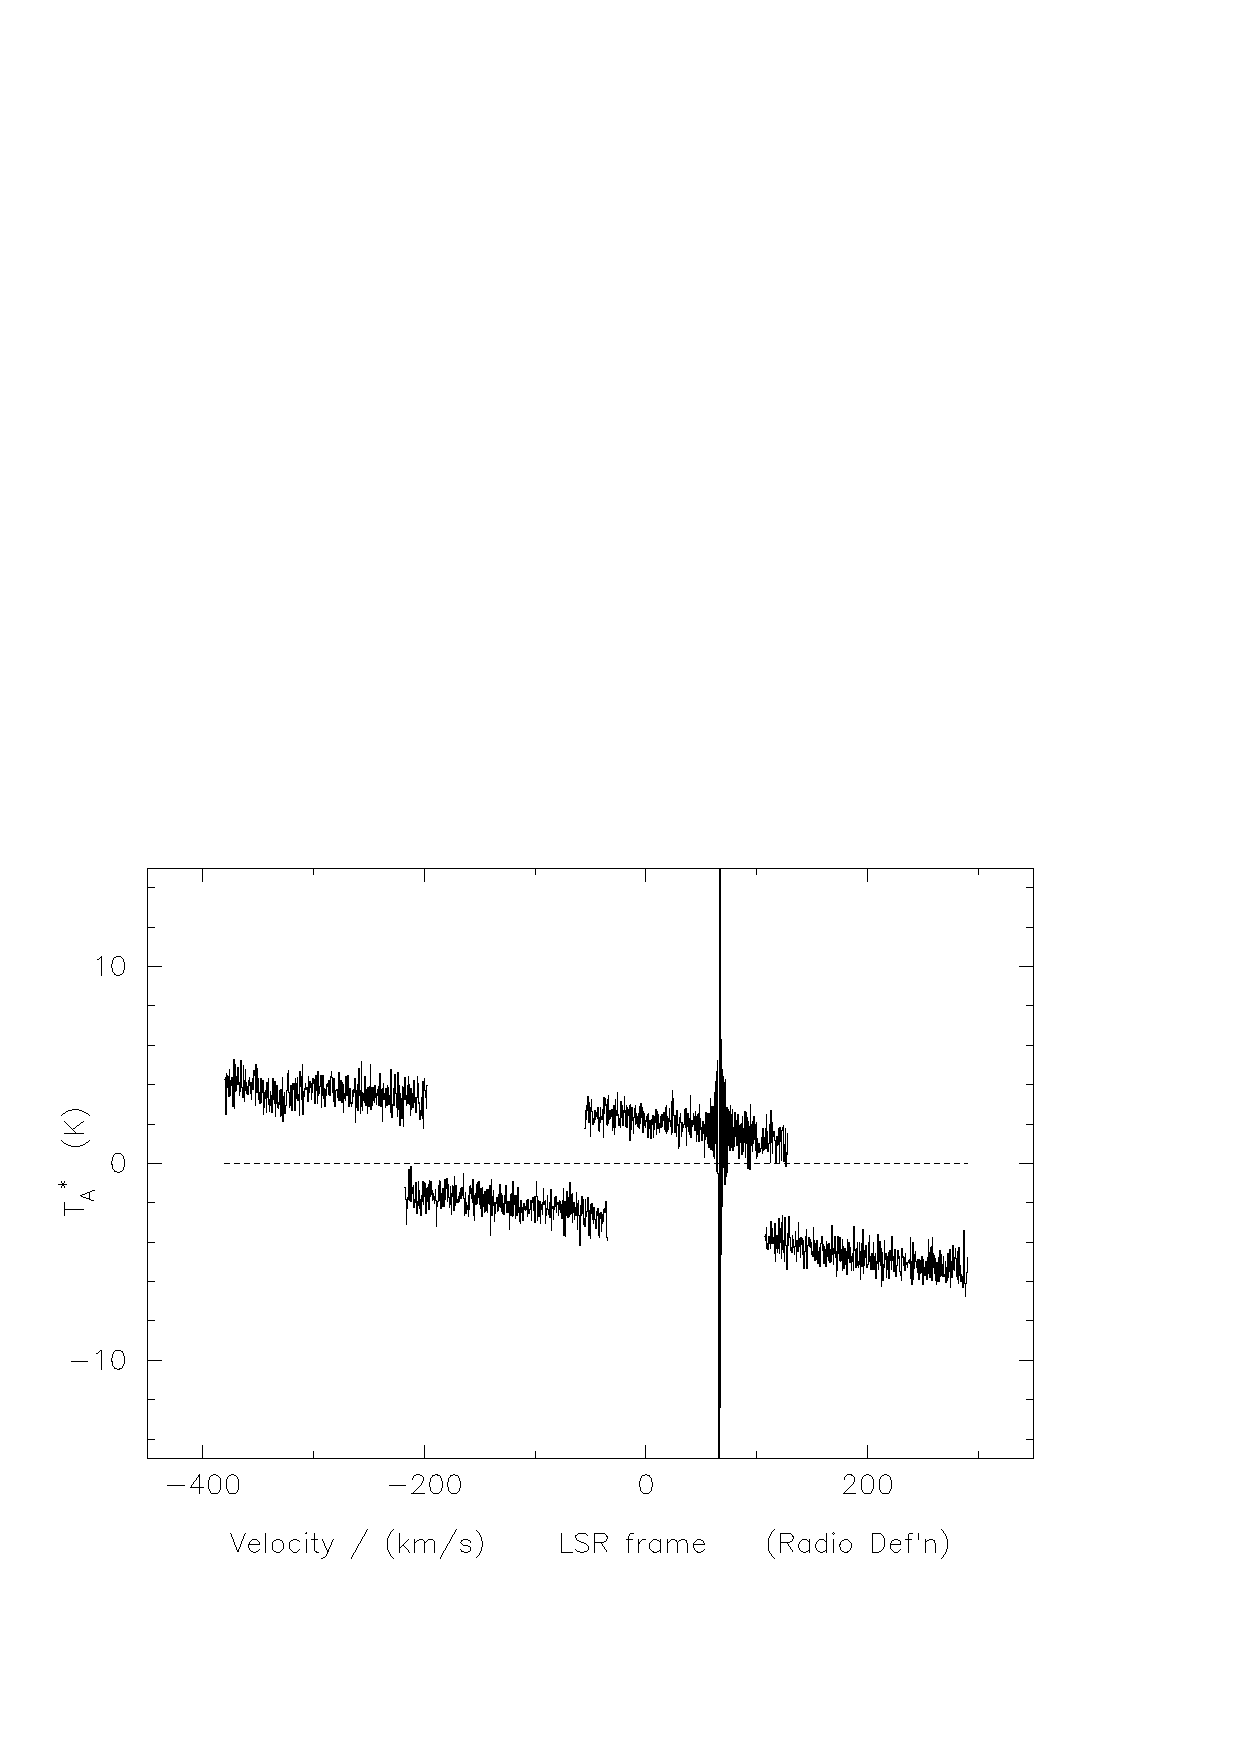
\includegraphics[width=0.8\textwidth]{sc8_dm_drop}
\caption[After \texttt{das-merge}]
{\small{The spectrum after applying \texttt{das-merge}. Quadrants offset
from one another for clarity.}}
\label{fig:after-das-merge}
\end{figure}

Note that the subbands still have significant overlap in velocity
space. This overlap is used to facilitate the second part of the \dm\
action, which averages signals in the overlap region. This can be done
separately using the \texttt{merge-quadrants} command. The end result in this
instance is shown in Figure~\ref{fig:dm_dasmerge}.
%
\begin{figure}[htb]
\centering
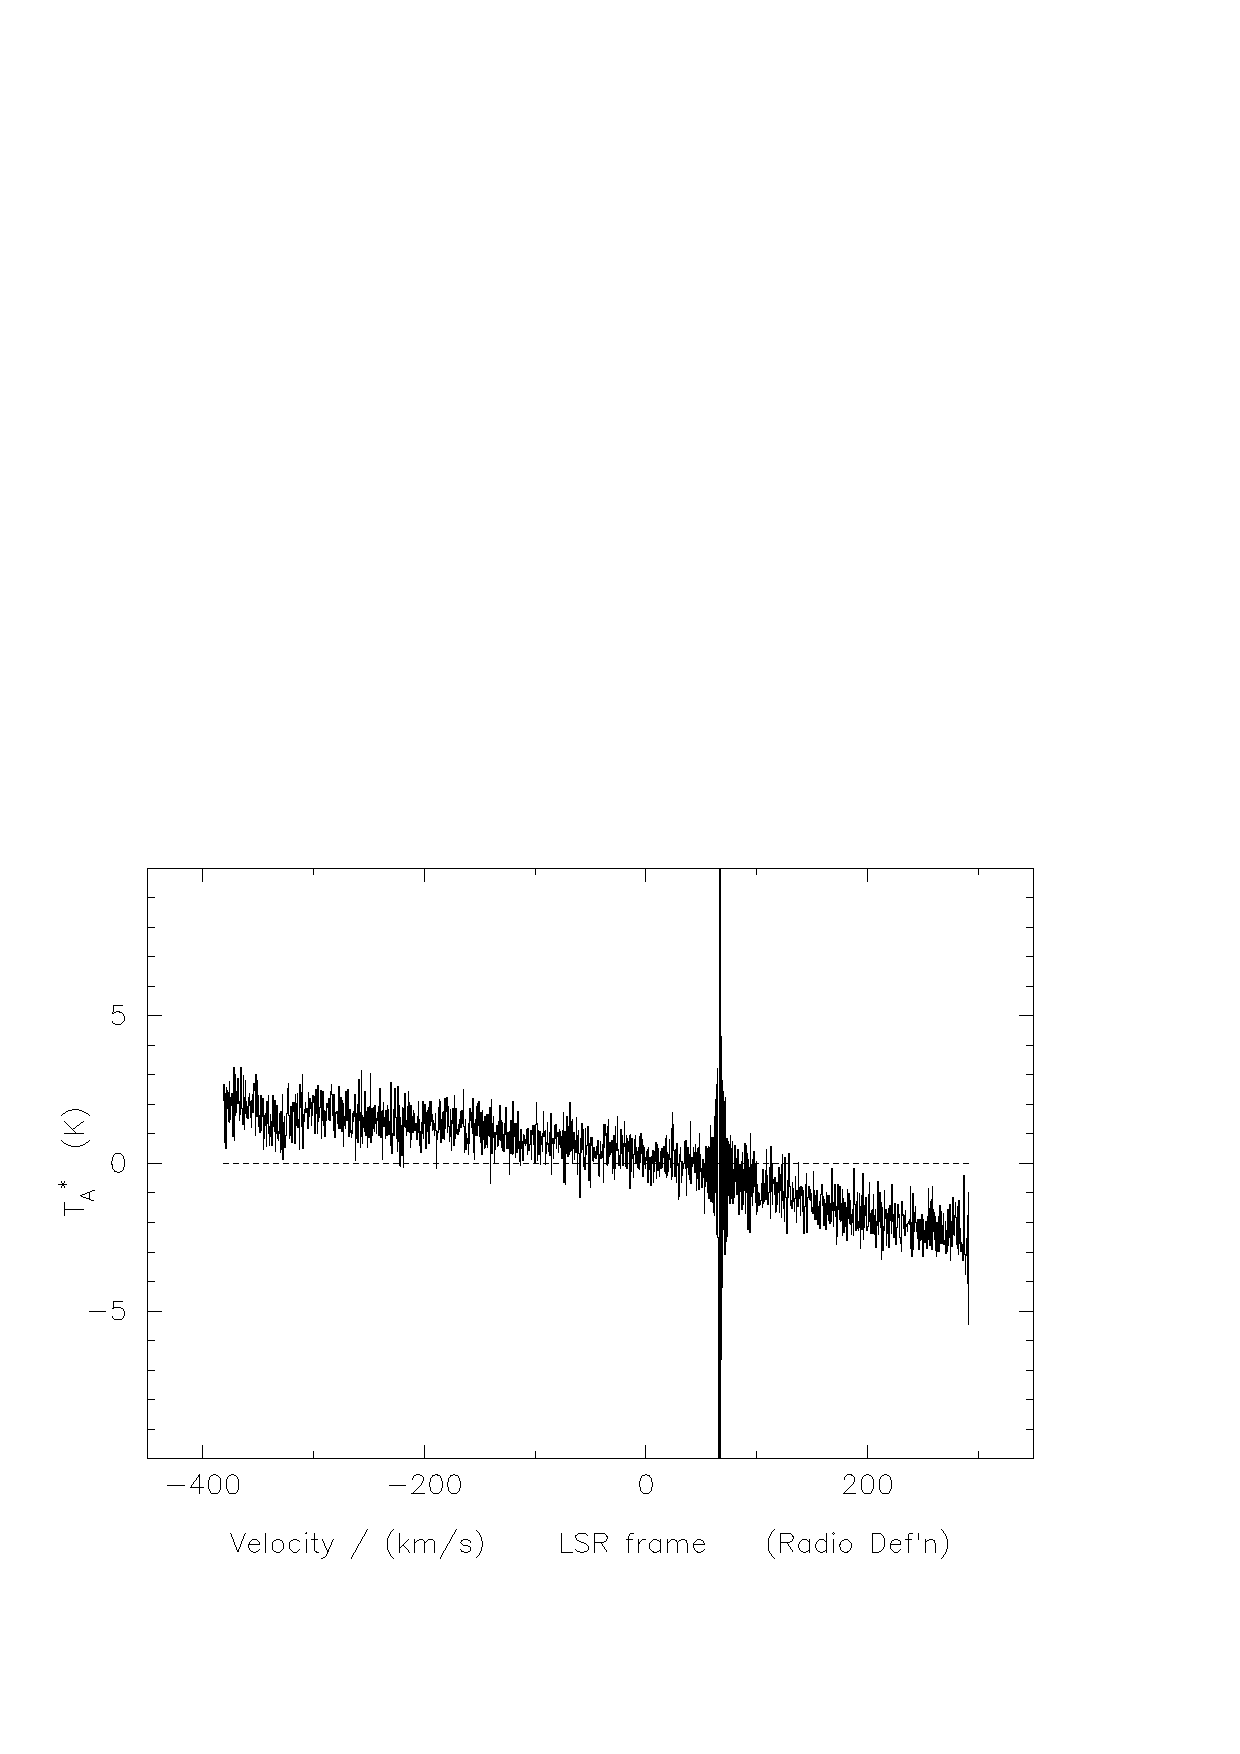
\includegraphics[width=0.8\textwidth]{sc8_dm_dasmerge}
\caption[Spectrum after \dm ]
{\small{The spectrum in Figure~\ref{fig:dm_dirty} after application of
\dm .  The subbands are successful merged into a continuous
spectrum. Only the interference spike remains.}}
\label{fig:dm_dasmerge}
\end{figure}

Note that if one has previously modified the effective rest frequency
using the \texttt{s-l-r-f} command (see Section~\ref{sec:s-l-r-f}) then one
must reset the rest frequency
to accept the default header values associated with the next spectrum
before \texttt{das-merge} can be used. That is, one must issue the
command

\SP\ \texttt{s-l-r-f 0.0}

first. The consequence of not doing this is that the first subband
of the new spectrum appears to \texttt{das-merge} to not have the correct
frequency, and the error message

\begin{terminalv}
 -- SPECX#033 -W- Can't MERGE - quadrants do not overlap --
\end{terminalv}

will result. This is your clue to the above common problem, if you
are given to mess with the frequencies.

\subsubsection{Caveats}
The defaults for \dm\ work well for most purposes; that is, taking the
default number of channels for removal, then refusing the vertical
adjustment between subbands. Long integrations suggest that it
is correct not to take the vertical subband adjustment.  The intrinsic
flatness of the DAS response is excellent, and applying the subband
adjustment actually can introduce low-level offsets between subbands,
which, particularly for wide weak lines, could result in spurious
detections.  Hence one should use the default command, equivalent to

\SP\ \texttt{das-merge$\backslash$\#$\backslash$n$\backslash$}

for almost all cases.

One particular case which can readily introduce baselevel offsets if one
applies the vertical subband adjustment is when one has a bright line
in the central overlap region. One such example is shown in
Figure~\ref{fig:dasmerge_yn}. In such case one should most definitely
use the default `{\tt{n}}' option.
%
\begin{figure}[ht]
\centering
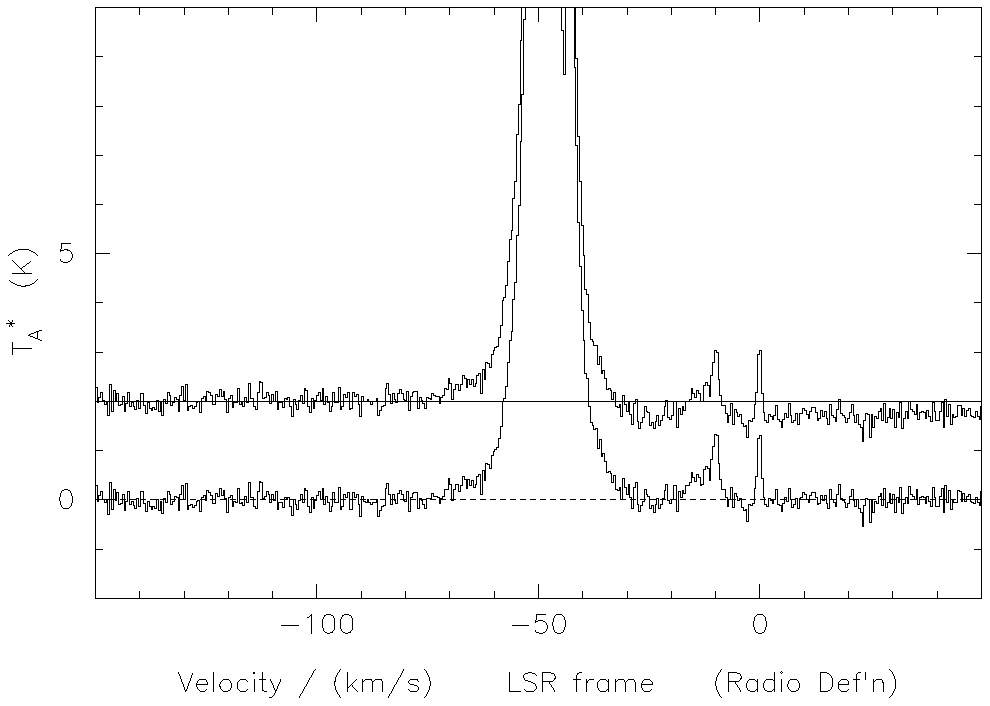
\includegraphics[width=0.8\textwidth]{sc8_dasmerge_yn}
\caption[\dm ; yes or no]
{\small{The same CO(3--2) spectrum of W3(OH), reduced using \dm\ with
subband offsets (upper spectrum) and without (lower spectrum). The
presence of the strong line in the overlap region introduces an
artificial baseline step in the former instance. One should use \texttt{das-merge$\backslash$\#$\backslash$n$\backslash$} here for sure.  }}
\label{fig:dasmerge_yn}
\end{figure}

Possibly the only time the `\texttt{n}' option may introduce artificial
effects is when observing a planet.  Even then the effect is likely to
be small. See Figure~\ref{fig:merge_diffs}.
%
\begin{figure}[ht]
\centering
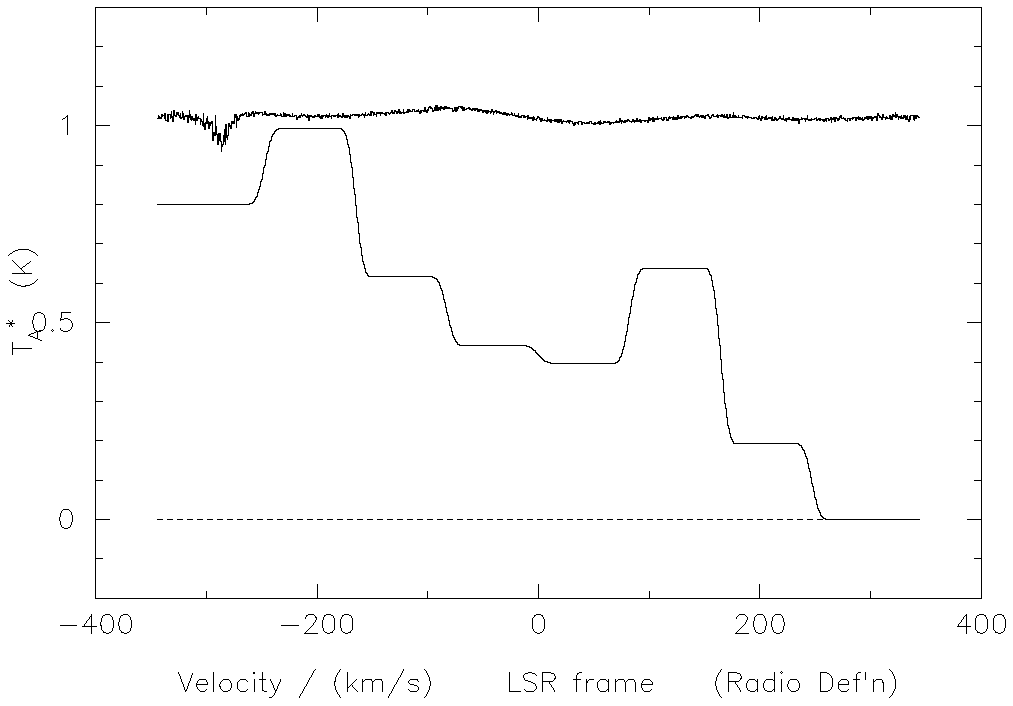
\includegraphics[width=0.8\textwidth]{sc8_merge_diffs}
\caption[\dm\ and planets]
{\small{The upper spectrum is an observation of Saturn using the
8-subband 760-MHz mode with B3i; the result is normalized to an
observed value of 90 K T$^*_a$ (\ie\ the actual value is about 45 K),
and subband offsets have been applied in this case when using \dm
. The lower curve shows the difference introduced when not using the
subband offsets, as compared with the upper spectrum. Using \texttt{das-merge$\backslash$\#$\backslash$n$\backslash$} here introduces
additional small steps corresponding to a maximum of about 1\% of the
total signal.}}
\label{fig:merge_diffs}
\end{figure}
%
%\end{document}



\subsection{Dealing With Multiple Spectra}
\label{sec:specx_8}
\subsubsection{Averaging Several Spectra}
\label{sec:specx_8.2}

SPECX is able to average only two spectra at a time.  If you want to
average several spectra you will have to do a little juggling with the
stack.

For example, if I want to average spectra 1 through 5, I would have
to do the following.  Read in spectrum 1, read in spectrum 2, average
them, read spectrum 3, average again, read spectrum 4, average, read 5
and average one more time.

Thus to average five spectra (131, 132, 133, 134 and 135, say) you
would type:

\SP\ \texttt{r-g-d 131}\\
\SP\ \texttt{r-g-d 132; ave}\\
\SP\ \texttt{r-g-d 133; ave}\\
\SP\ \texttt{r-g-d 134; ave}\\
\SP\ \texttt{r-g-d 135; ave}

Generally, if you have learned to put all the necessary commands on
one line you can repeat the sequence of using the `up-arrow' key and
editing the line. If you have to do it very often, it would probably
be smart to write a command file (see Section~\ref{sec:specx_9}) or an
in-line do-loop (see Section~\ref{sec:do-loops}) to do it for
you. Such a do-loop might go like this:
\begin{terminalv}
>> r-g-d 131
>> do i 132 133
 Enter commands to do, line at a time, EOF to finish
 insert >> r-g-d i
 insert >> ave
 insert >>
\end{terminalv}
This would then average your spectra. Certainly less typing if you
have a lot of spectra in sequence(s) to average. Note that having done
the do-loop once creates a file called \texttt{temp.spx} which does the
same thing as the do-loop we just made. So if you had two more groups
of spectra (say, 138--143 and 145--150) to average with the preceding
average, just type

\SP\ \verb|@temp 138 143|\\
\SP\ \verb|@temp 145 150|

to complete the set of spectra to be averaged.

\subsubsection{Displaying More Than One Spectrum}
\label{sec:specx_8.3}
In Section~\ref{sec:specx_5.2} there are some plots with more than one
spectra. The ability to plot two or more spectra on one set of axes is
very useful sometimes.

When you send the \texttt{new-plot} command \SPECX\ closes the old plot
file and opens a new, clean one.  The trick of getting more than one
spectra is not to close the plot before you're done adding things to
it. This is done using the \texttt{overlay} command, as we have already
seen. There is a \texttt{close-plot} command by the way, which is useful
particularly when you are working with output to a plotfile ultimately
destined for printing.

You can keep on using \texttt{overlay} for any number of spectra. If you
want a decent plot remember to offset them vertically one from another
(use the \texttt{offset} command). Also, you can't change the plot scales
after you've opened a plot so make it big enough before you start.

\subsection{Concatenation -- combining spectra lengthwise}
If you have several independent spectra for which the
velocity/frequency ranges are cover a wider range than any one such
spectrum, it may be useful to combine them on a single plot. This is a
trivial application, since all one has to do is increase the length of
the x-axis of the final plot sufficiently to allow yourself room to
plot all the spectra using \texttt{new-plot} and successive applications
of \texttt{overlay}. There are however, a couple of more specialised
applications, which we get to next.

\subsubsection{Making very long spectra}
\label{sec:long-spectra}
There is a much less trivial application than the above which occurs
when one has spectra which occupy both sub\textit{systems} of the \das .
Consider a CO 4-3 observation with receiver C2 in the
special wideband mode; in this case there are 16 subbands, using both
subsystems, and extending over nearly 1.8 GHz. Each subsystem consists
of eight subsections.  Loading this spectrum into \SPECX\ shows that
\textit{two} positions in the stack are used, one for each subsystem:

\begin{terminalv}
 >> r-g-d 46
 GSD version  5.3
          (x,y) offset = ( 159.9,   0.5) arcsec
          rotation angles: x2y =  -90.0 deg.; v2y =    0.0 deg.
          (r,d) offset = ( 159.9,   0.5) arcsec


 Stack posn    Scan no    Title
     X           46      0046.000_B  SATURN   JCMT
     Y           46      0046.000_A  SATURN   JCMT
 >>
\end{terminalv}

The following sequence of commands will reduce this to a single
spectrum (dialogue has been omitted):

\begin{terminalv}
>> r-g-d 46
>> das-merge\#\n\
>> xy
>> das-merge\#\n\
>> xy
>> concat
>> merge-quad\n\
\end{terminalv}

Here one first performs the \texttt{das-merge} on each of the subsystems
separately, then concatenates the two spectra to produce a single
version which has overlapping channels around the centre, and finally
merges both spectra together to form the final result. Normally the
comamnd \texttt{merge-quadrants} is used only as part of \texttt{das-merge},
but it can be used separately, as in this instance.

Doing this to the next spectrum, averaging the result, and so on for
all the spectra in a set one can form the final average (see
Figure~\ref{fig:concatenation}). It would make sense to construct a
procedure to do this (see later).

\begin{figure}[htb]
\centering
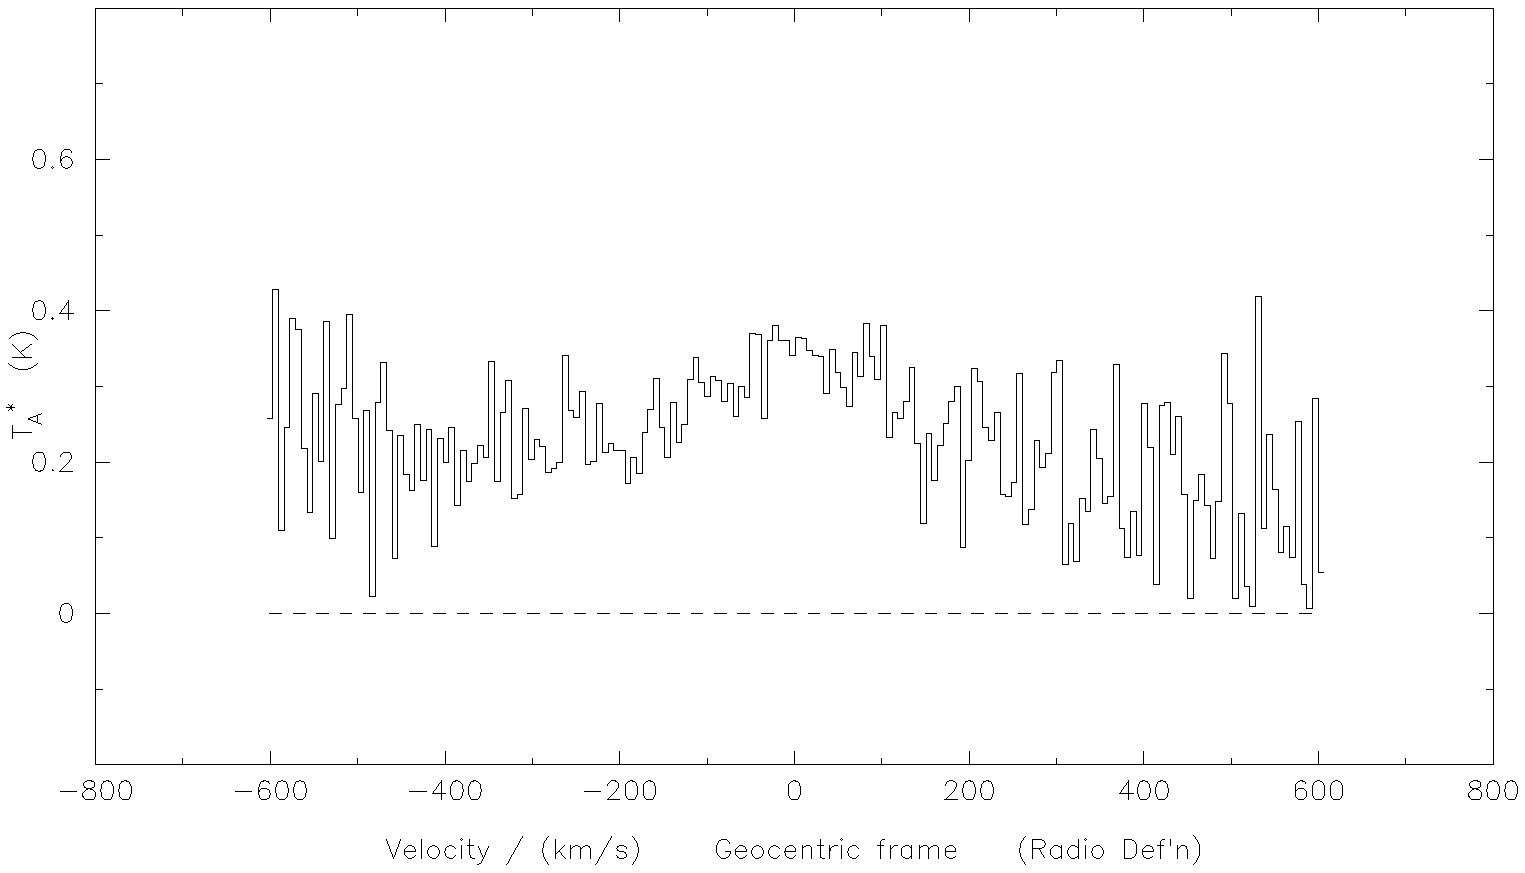
\includegraphics[width=0.8\textwidth]{sc8_concat}
\caption[Extreme wideband spectra (concatenation)]
{\small{An example of a spectrum taken in the dual subsystem mode with
receiver C2, covering about 1.8~GHz, after concatenating and merging
the two subsystems.
 }}
\label{fig:concatenation}
\end{figure}

\subsubsection{The special case of the 750-MHz mode}
The 750-MHz mode of the \das\ was used for a short time only for
receiver A2, and is no longer in use. In this case there were two
subsystems of 4 subbands each. A similar approach can be taken in this
case, to that used for the ultra-wideband mode discussed above.

\subsection{Arithmetic With Spectra}
\label{sec:specx_8.1}

As you saw before when I was removing baselines, you can subtract the
\texttt{X} register from the \texttt{Y} register and have the difference
become the new \texttt{X} register.  The command is \texttt{subtract-spectrum}.  \SPECX\ can also add the \texttt{X} and \texttt{Y}
together and average them.  The commands are \texttt{add-spectrum} and
\texttt{average-spectrum}.  \texttt{average-spectrum} ({\tt{ave}} is enough)
is the usual choice, and uses weights when averaging that are
determined by the integration time divided by the square root of the
system temperatures of the two spectra.

While I'm on the subject, \SPECX\ also has \texttt{multiply-spectrum} and
\texttt{divide-spectrum}.  Skipping the conversational mode the commands
would be \eg :

\SP\ \verb|mult 2.0|

and

\SP\ \verb|div 7.8|

The defaults factors are set to unity (they used to be zero).

\subsubsection{Spectrum Statistics}
\label{sec:specx_10}
At some point during your data reduction you might want to know a little more
about your spectrum.  There are several commands which determine the
parameters of spectra.  Two of the more useful commands are \texttt{find-spectrum-statistics} and \texttt{find-integrated-intensity}.  There are
others in R. Padman's manual.

To use these commands in interactive mode you get a plot of the
current spectrum like you did when removing and fitting baselines so
that you can specify a region.  Just use the cursor or crosshairs and
\texttt{l}, \texttt{r}, and \texttt{a} as you did before.

Once again it may be useful to write the outputs to a separate file
using the \texttt{s-l-f} command.

\subsection{Dealing with spikes}
\label{sec:spike-removal}
External (or internal) interference (RFI) is a common occurrence with
the longer wavelengths in use at the JCMT; that is, particularly in
spectra taken with receiver A2. Usually this is offset from the centre
of the band and is of no major concern. It seems to be worse for
position-switching and may disappear entirely in the azimuth
beamswitched mode. Sometimes, however it can be a real nuisance. An
example is given in Figure~\ref{fig:spikes}.

\begin{figure}[htb]
\centering
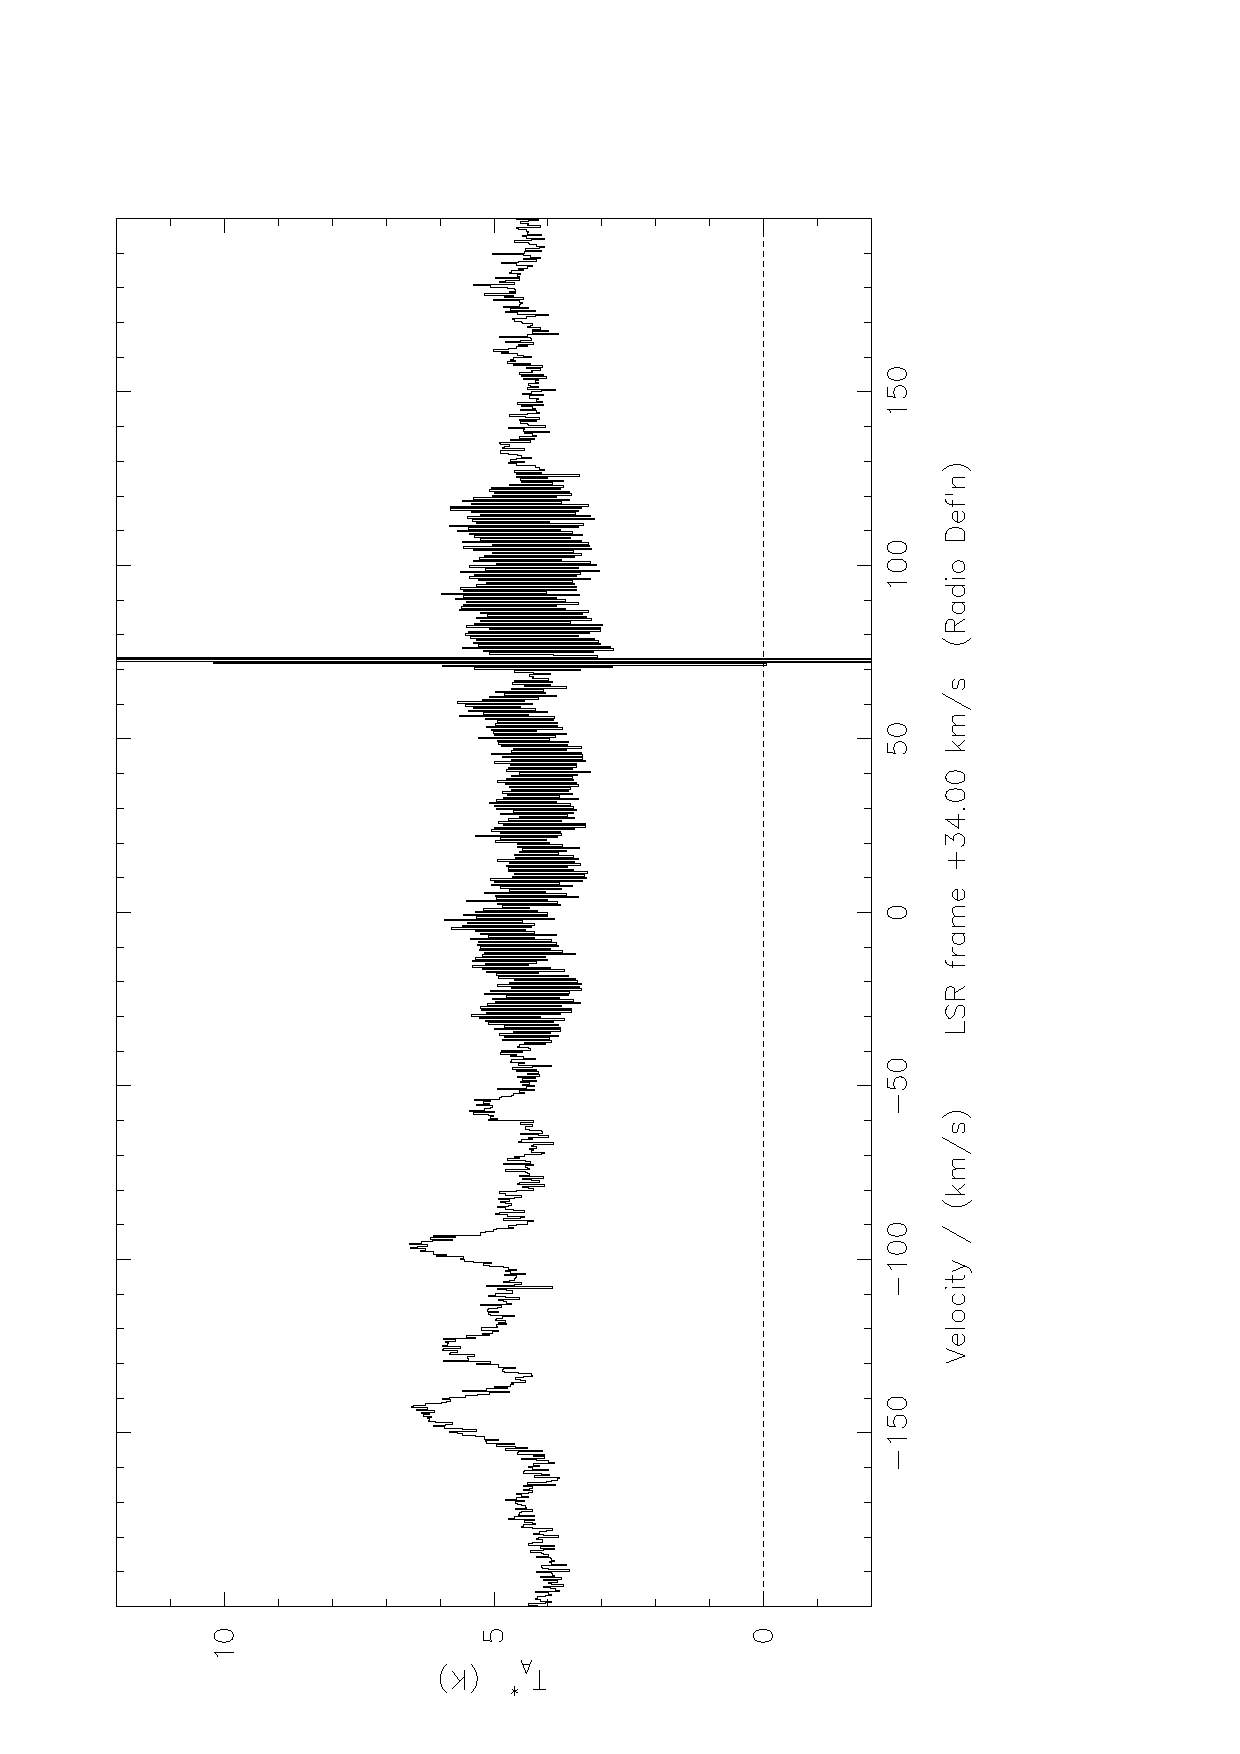
\includegraphics[width=0.8\textwidth]{sc8_spiked}
\caption[`Ringing' in a spectrum]
{\small{A position-switched \das\ spectrum of G34.3 in the area of
239~GHz showing `ringing' caused by a strong internal interference
spike. Note that it affects only the subband in which it occurs. The
offset from zero is the result of a combination of the source
continuum emission and a difference in the airmass between the signal
and reference positions. The line features are due to CH$_3$CCH and
CH$_3$CN.  }}
\label{fig:spikes}
\end{figure}

Such interference spikes may be very effectively removed by applying
Hanning smoothing to the spectrum:

\SP\ \texttt{hann}

The result is shown in Figure~\ref{fig:despiked}. A multitude of weak
line features, as expected, are now revealed. The spike itself may be
removed by using the spike-removal command:

\SP\ \texttt{rem-spike}

\begin{figure}[htb]
\centering
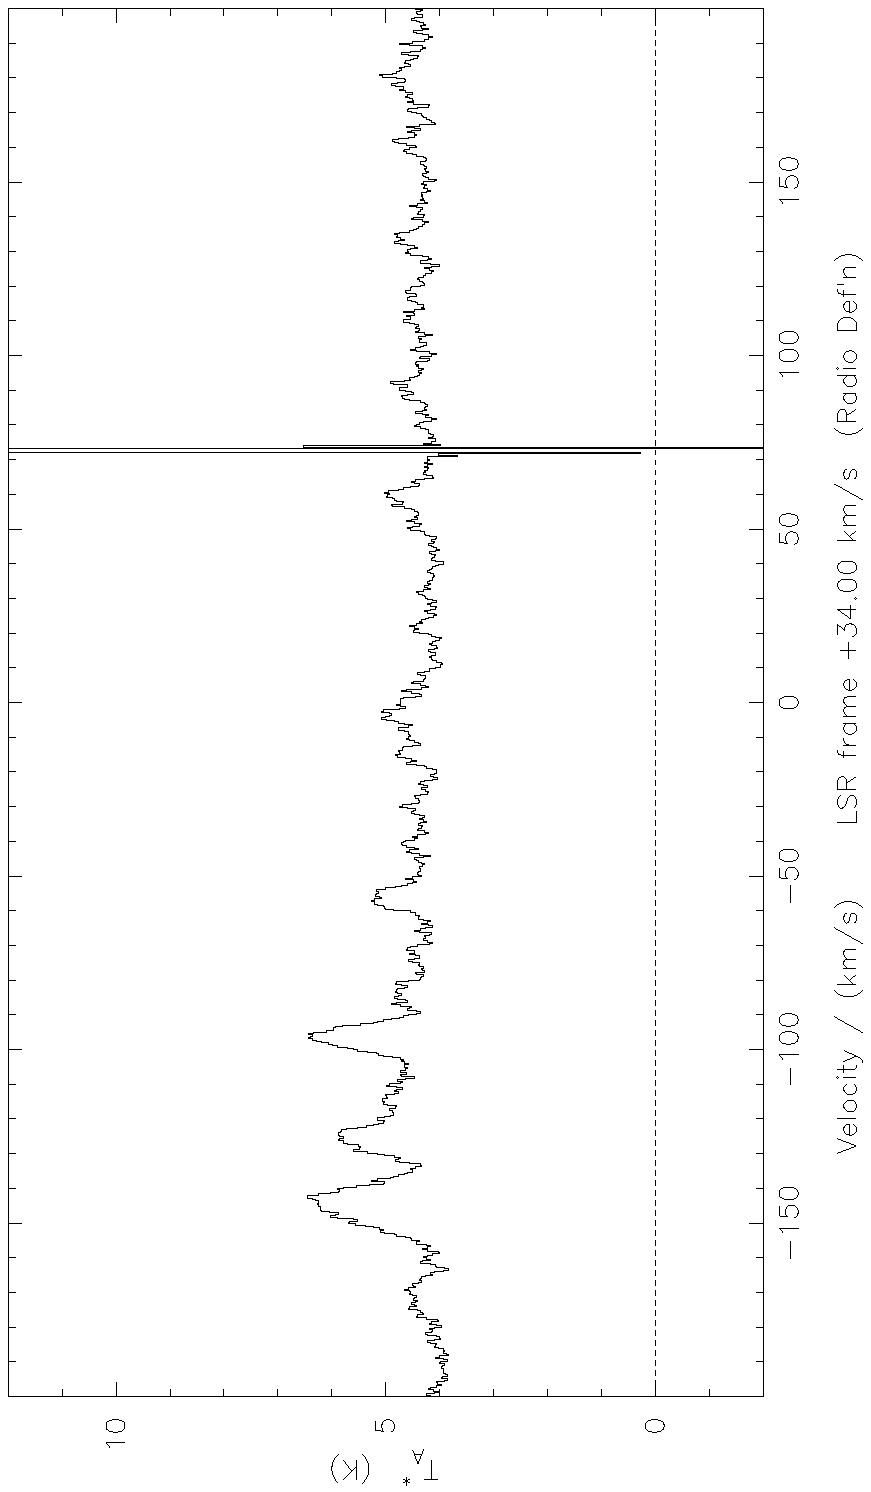
\includegraphics[width=0.8\textwidth]{sc8_despiked}
\caption[Hanning-smoothing removes `ringing']
{\small{The result of applying Hanning smoothing to the spectrum shown
in Figure~\ref{fig:spikes}. Note that the `ringing' completely
disappears, revealing previously obscured line features. The spectrum
is itself somewhat smoothed in the process.  }}
\label{fig:despiked}
\end{figure}




\subsection{Writing Your Own Command Files}
\label{sec:specx_9}
To save time and keystrokes when reducing your data, you can write
command files that will do the tedious work for you.  When writing
command files it is usually faster to be outside of \SPECX . To do
this you can either do
\begin{enumerate}
\item
\SP\ \verb|exit|; which will take you out of \SPECX\ completely, or
\item
\SP\ \verb|$|\\
\verb|Shell command line?|

This is your cue to enter any shell command that you would like, such
as, say,

\begin{terminalv}
emacs &
\end{terminalv}

to start up \texttt{emacs} in a separate window which will remain until
you specifically close it.
\item
You can just type this without asking for the prompt, of course:

\SP\ \verb|$ emacs &|

\item
If you are using a windowed terminal, open a completely separate \texttt{xterm}, say, for the purpose.
\end{enumerate}

A command file is very simple to understand because it's just a list of
\SPECX\ commands.  The only pitfalls are knowing what order to submit the
commands to \SPECX\ and knowing in advance what questions \SPECX\ is
going to ask. This implies a little experience is useful before trying
to write your own command procedures. Which is why this information is
not placed earlier in this Cookbook.

\subsubsection{The Basics}
\label{sec:specx_9.1}
Here's a simple example of a command file.  I want \SPECX\ to read
observation number 137, das-merge it, smooth the data over a 5 point
average, and plot it.  First, here are the commands that one would
give in \SPECX :

\SP\ \verb|r-g-d 137| \\
\SP\ \verb|das-merge\\n\ | \\
\SP\ \verb|sm-sp 5| \\
\SP\ \verb|n|

These lines would be faithfully reproduced in a command procedure.
You would type, say:

\begin{terminalv}
$ pico
\end{terminalv}
% $
in a separate \texttt{xterm} window and you will be in the \texttt{pico}
editor. The latter is simple because there are rather few commands and
the basic ones are always displayed at the bottom of the editing
window. If you have an aversion to the complexity of \texttt{emacs} this
may be the one to use. Now just type the same one line entries as you
would inside \SPECX . When you are done type \texttt{Control-o} and you
will be prompted for the file name you want to write out ({\tt{a.spx}},
say, remembering that all \SPECX\ command files are of filetype \texttt{.spx}) Now the file \texttt{a.spx} has been created.  To use it, I get
back into \SPECX\ either by clicking back on your \SPECX\ window.

Then, back inside \SPECX\ type

\begin{terminalv}
@a
\end{terminalv}

The \texttt{@} tells \SPECX\ to start running a command file.  Notice you
do not use the suffix \texttt{.spx} in the command.

This was a very silly command file so let's write one that is a little
more useful.

%**********

\subsubsection{Repetitive Operations}
\label{sec:specx_9.2}

You will recall that when you want to remove a linear baseline from a
spectrum or do a similar operation, you had to tell \SPECX\ what
region(s) to use from the spectrum.  This would hinder automatic
operations severely since you would have to sit at the terminal and
use the cursor to tell \SPECX\ what regions to use.  The way out of
this is to always use non-interactive mode:

\begin{terminalv}
>> set-interactive
Interactive plotting? (Y/N) [Y] N
\end{terminalv}

Now \SPECX\ can carry out things like \texttt{remove-linear-baselines}
without plotting the spectra on the screen, and asking lots of
questions first.  The advantage is when you want to use the same
regions for removing baselines, or a similar operation like \texttt{find-spectrum-statistics} in several spectra.  For instance, I want to
use the regions from $-40$ to $-20$ km/s and from 20 to 40km/s for
removing a linear baseline from several spectra, put them into a file
called \texttt{gooddata.sdf} and have it repeat the command until I'm
done.  I would write the following command file, which I'll call \texttt{rlb.spx}:

\begin{terminalv}
r-g-d\?\
r-l-b\-40 -20\20 40\
wr-sp\1\
\end{terminalv}

The \texttt{?} in the first line will prompt me for a scan number every
time I run the command file. I have specified the linear baseline fit
regions between the backslashes, which indicate where responses are be
expected to
anticipated questions from the
\SPECX\ command. I put the data in file number \texttt{1} with the \texttt{wr-sp}
command, which is \texttt{gooddata.sdf} (I'm assuming you had no other open
files). To run the command file type

\SP\ \verb|@rlb|

and \SPECX\ will ask which scan you want to read (because of the \texttt{?}).
Alternatively, you could type, say,

\SP\ \verb|@rlb 137|

and the file will process scan 137, without any further ado.

\subsubsection{Automatic Repetitive Operations}
\label{sec:specx_9.3}
In the example above, say I want to make a list of the scans to be
read in so that I can change the list when I want and go out for
doughnuts while \SPECX\ does all the work.  One could combine a number
of calls to the command file \texttt{rlb.spx} in a simple-minded way in a
new command file \eg\

\begin{terminalv}
@RLB 101
@RLB 102
\end{terminalv}
\vspace*{-0.1in}
\vdots
\vspace*{-0.1in}
\begin{terminalv}
@RLB 119
@RLB 120
\end{terminalv}

Saving this command with some name (say, \texttt{1to20.spx}) and running it
by typing

\SP\ \texttt{@1to20}

processes each of the scans 101 through 120, placing the results in my
output file. \SPECX\ will start running \texttt{1to20.spx}; the first command
it gets is to run \texttt{rlb.spx}, and while running \texttt{rlb} it sees
the \texttt{?} and looks for a value, it finds the value in \texttt{1to20.spx} and continues to run happily along until it gets to the end
of \texttt{1to20.spx}.

This is still a bit silly. Since \SPECX\ allows the use of loops and
counters, one can achieve the same result a lot more elegantly. That
is, if one creates a command file (call it, say, \texttt{doit.spx}):

\begin{terminalv}
do n 101 120
r-g-d\n\
r-l-b\-40 -20\20 40\
wr-sp\1\
enddo
\end{terminalv}

then typing

\SP\ \verb|@doit|

will achieve the same result. The counter \texttt{n} will step from 101
to 120.

As you might guess \texttt{doit.spx} could look like this also:

\begin{terminalv}
do n 101 120
@rlb\n\
enddo
\end{terminalv}

Taking this still one step further allows the input of parameters from
outside:

\begin{terminalv}
declare fscan i4
declare lscan i4
ask 'First scan?',fscan,?
ask 'Last scan?',lscan,?
do n fscan,lscan
@rlb\n\
enddo
\end{terminalv}

In this case running this procedure will prompt you for the first and
last scans to be processed by \texttt{rlb.spx}. Note that (a) the
declaration of the type of variable (I4) required by \SPECX\ for
input, and (b) the use of the \texttt{ask} command. The latter gives a
prompt (\eg\ \texttt{First scan?}) and puts your answer in \eg\ the
variable \texttt{fscan}.

\subsubsection{In-line do-loops}
\label{sec:do-loops}
A useful variant of command procedures is an \textit{in-line do loop};
that is, a set of repetitive operations performed once only without
making a command file. To make such a file one begins with a simple do
loop statement. Then one is prompted to type in commands, ending with
\ctrld (EOF). For example, say I want to move a sequence of spectra
from a map file and write then to an open file. I might do it this
way:
\begin{terminalv}
>> do i 1 8
 Enter commands to do, line at a time, EOF to finish
 insert >> g-s-f-m i
 insert >> wr-sp 1
 insert >>
 Filed as scan  31 of junk
 Filed as scan  32 of junk
 Filed as scan  33 of junk
 Filed as scan  34 of junk
 Filed as scan  35 of junk
 Filed as scan  36 of junk
 Filed as scan  37 of junk
 Filed as scan  38 of junk
 >>
\end{terminalv}
Using the variable \texttt{i} as a simple counter, I read the series of
spectra from the map and write then to file number 1. Because there
are already spectra in this file, the scan numbers increment from the
previous last number.

I mentioned that the in-line do loop is used only once. However,
that's not necessarily true. Such a command file leaves a record of
itself in a file called \texttt{temp.spx}. Naturally Unix overwrites this
file every time a new version is created, so if you wanted to keep
such a file you would have to rename it. The version of \texttt{temp.spx}
created by the preceding simple do loop looks like:

\begin{terminalv}
 do i                   1   10    1
 g-s-f-m i
 wr-sp 1
 enddo
 return
 >>
\end{terminalv}
This routine could be re-used by simply typing

\SP\ \verb|@temp|

In-line do-loops are really quite useful. It's up to your imagination
what you use them for.


\subsection{Modifying the Velocity and Frequency Axes}
\label{sec:modifying-axes}
There are occasions when it is helpful to change the x-axis on a
spectrum. This is particularly true for observations made with offset
frequencies designed to accommodate two or more spectral lines from
the same or different sidebands. There are four commands which are
very useful in this respect:
\begin{enumerate}
\item
\verb|set-x| enables one to change the x-axis scale;
\item
with \verb|set-line-rest-frequency| it is possible to modify the plot
so that the spectrum appears as if this frequency had been chosen as
the rest frequency
\item
\verb|set-velocity-frame| lets one enter a velocity to which the
spectrum will be referred in subsequent plots;
\item
\verb|change-sideband| shows the spectrum as if it were referred to
the other sideband. Use of this command \textit{frees the x axis plot
scale}; to return it to the original setting you will have to undo
this effect with \texttt{s-p-sc}.
\end{enumerate}
The effects of these commands tend to cause confusion sometimes, so it
may be useful to discuss them a little more. The last three can best
be discussed together.  One important thing to realise is that the
header values of the spectrum are not changed by any of these
commands, just the relative positioning of the spectrum in
velocity/frequency space for the purpose of plotting. Some parameters,
but not all, are carried over into the headers of stored reduced
spectra and map files.

\subsubsection{\texttt{set-x}}
\label{sec:set-x}
\SPECX 's default state on startup is to make all spectrum plots with
the x-axis as velocity. This may not always be what you want for
clarity, and the command \texttt{set-x} is provided to enable one to plot
with a different x-axis. There are three main choices: points,
frequency, and velocity. The `points' option is useful for determining
which channels to lose from the spectrum if you are planning to make a
map.

For instance, the spectrum below (Fig.~\ref{fig:set-x-orig})
is typical of those obtained toward
OMC-1. Within the band are two lines in which I happened to be
interested at the time, neither of which will appear at the expected
velocity, because the observing frequency was chosen to allow both
lines to appear in the band, and a non-standard \das\ mode was used
for the observation.

\begin{figure}[ht]
\centering
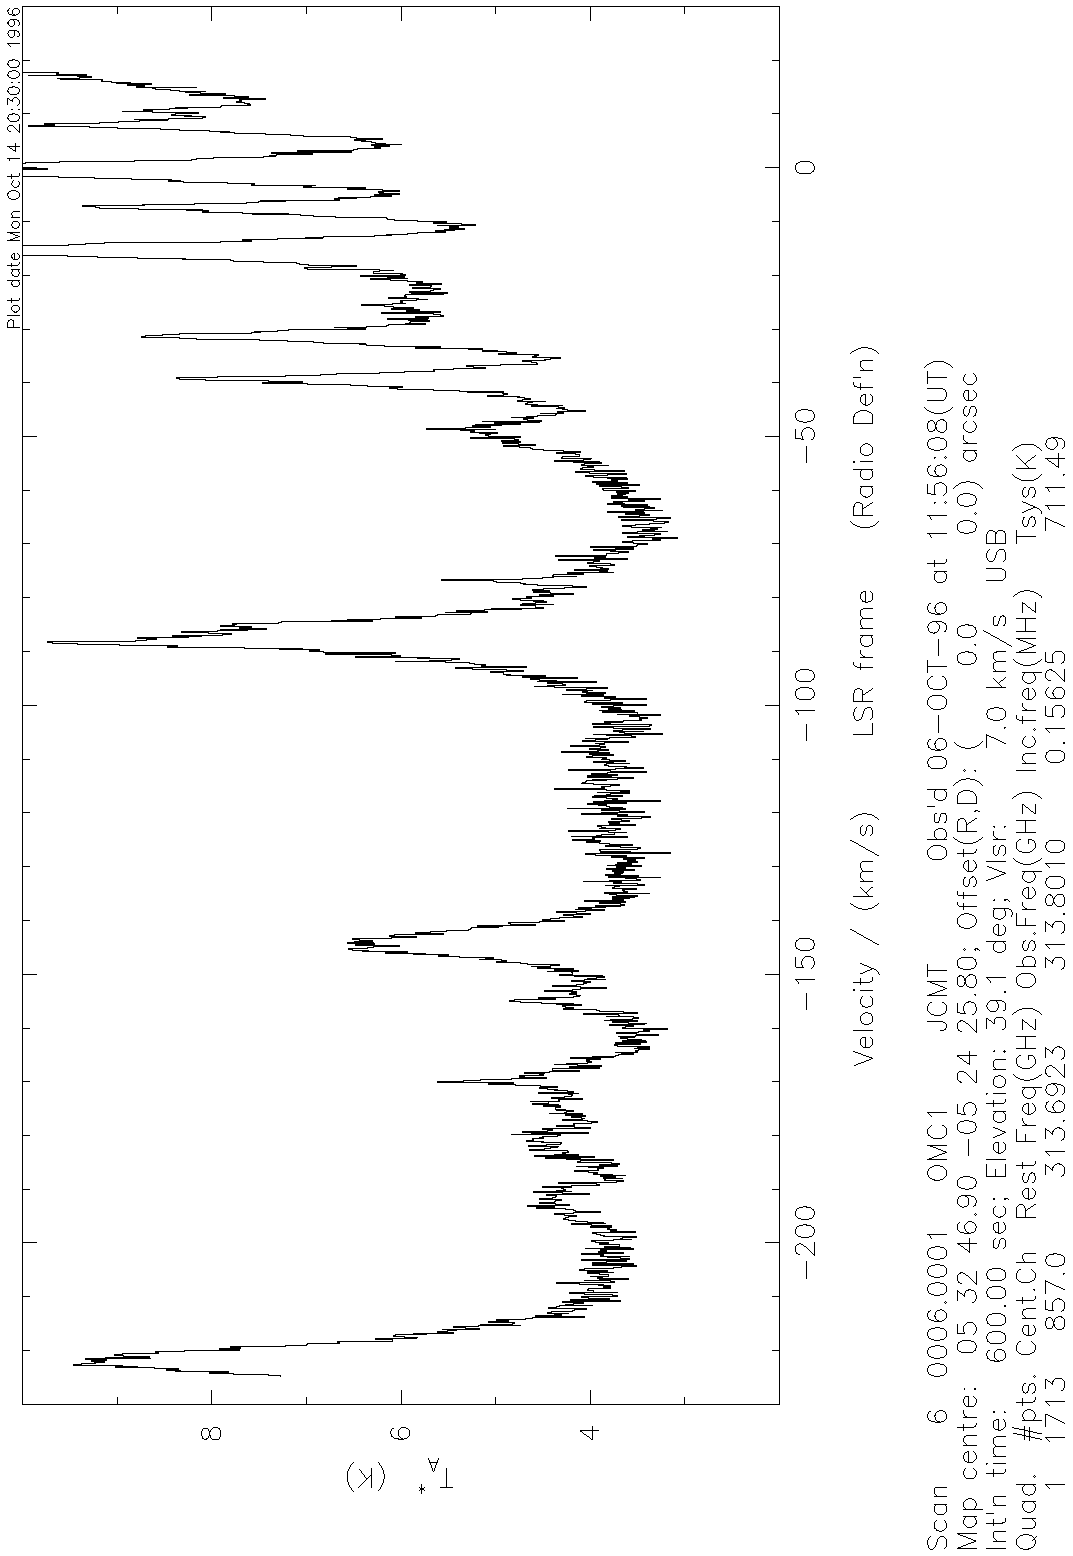
\includegraphics[width=0.8\textwidth]{sc8_hdo-orig}
\caption[A messy spectrum]
{\small{The result of observing with an offset frequency in a
line-rich source.
}}
\label{fig:set-x-orig}
\end{figure}

The two lines (of HDO) are at about $-50$ and $-145$~km/s
respectively, but it is rather messy to work this out at altitude.  It
is actually more useful to work in frequency in this case. So,
to change from velocity scale to a frequency scale, use \texttt{set-x}
and the following exchange occurs:

\begin{terminalv}
 >> set-x

 Set units for X-scale:
 Key:    1      Points scale
         2      Frequency scale
         3      Velocity scale
         4      User defined scale

    Current units are km/s

 Key?  [3] 2
 Apply polynomial correction to frequency scale? (Y/N) [N]
 Absolute or relative frequencies? (A/R) [R] a

 X-scale units set - GHz
\end{terminalv}

Note that there is more to this command than just choosing an
x-axis. One must also choose the origin, effectively, in this case via
the absolute/relative frequency switch. If I had chosen `relative' I
would have been asked ``relative to what?''.

In this example I chose to turn off the polynomial frequency
correction; having this on is useful only for non-linear scales such as
that produced
by the \aosc . The \das\ scale is quite linear by definition. The use
of absolute frequency scales enables me easily to see what frequencies
my lines have. As shown below in Fig.~\ref{fig:set-x-to-freq},
this provides both upper and lower
sideband frequency scales, on the bottom and top x axes
respectively. However, these scales will be correct \textit{only if one
puts in the correct peculiar velocity for your source}; otherwise a
velocity of 0 km/s is assumed. Thus if the lines have an appreciable
peculiar velocity they will appear to have the incorrect
frequency. The velocity is specified by using \texttt{s-v-f}. This
therefore brings us to the next section.

\subsubsection{\texttt{s-l-r-f}, \texttt{s-v-f} and \texttt{ch-sid}}
\label{sec:s-l-r-f}
So, if I put the correct velocity in place using \texttt{s-v-f}:
\begin{terminalv}
 >> s-v-f
 Output in different vel frame? (Y/N) [N] y
 Velocity frame? (TELLuric, LSR, HELIocentric, GEOcentric) [ LSR]
 Velocity law definition? (OPTical, RADio, RELativistic) [RAD]
 Velocity in new frame? (km/s) [  7.00]
 >>
\end{terminalv}
and then changing the x-axis to frequency using \texttt{set-x} we get the
result following in Fig.~\ref{fig:set-x-to-freq}:

\begin{figure}[ht]
\includegraphics[width=0.8\textwidth]{sc8_hdo_freq}
\centering
\caption[A messy spectrum with reasonable axes]
{\small{Figure~\ref{fig:set-x-orig} after changing to a frequency
x-axis and providing \SPECX\ with the correct lsr velocity.
}}
\label{fig:set-x-to-freq}
\end{figure}

From these data the two HDO lines at 310.5333 (upper x axis; lower
sideband) and 313.7506~GHz (lower x axis; upper sideband) are clearly
seen to be present. Of course, the spectrum is reversed now because of
the change in axis coordinate, but it makes line identification a lot
easier. A subsequent observation at a shifted velocity confirmed this
result on this occasion.

Just to show that this all works as expected, we can use a combination
of setting the correct line rest frequency (with \texttt{s-l-r-f}) and
adopting the other sideband (using \texttt{ch-sid} as appropriate) to display
the two
lines of interest to good advantage. In this I anticipate the
questions \SPECX\ will ask. Then for the line in the \textit{upper sideband}
at
313.7506~GHz:
\begin{terminalv}
 >> s-l-r-f 313.7506
 >> s-v-f \y\lsr\rad\7.0\
 >> n

 Plot opened; sequence no. 024

 Warning ** Rest frequency set using values from SET-LINE-REST-FREQ.
 Do S-L-R-F. to use defaults from header

 -- sxgdevice --/xwindow         SPECXDIR:SPECX_PGPLOT.PS
 >>
\end{terminalv}

Note the warning \SPECX\ issues, to let you know that you have
modified the frequency/velocity scale. If you want to revert to the
default settings you need to type \verb|s-l-r-f 0.0|. Taking a
narrower velocity range the plot looks like that in Fig.~\ref{fig:set-to-usb}:

\begin{figure}[ht]
\centering
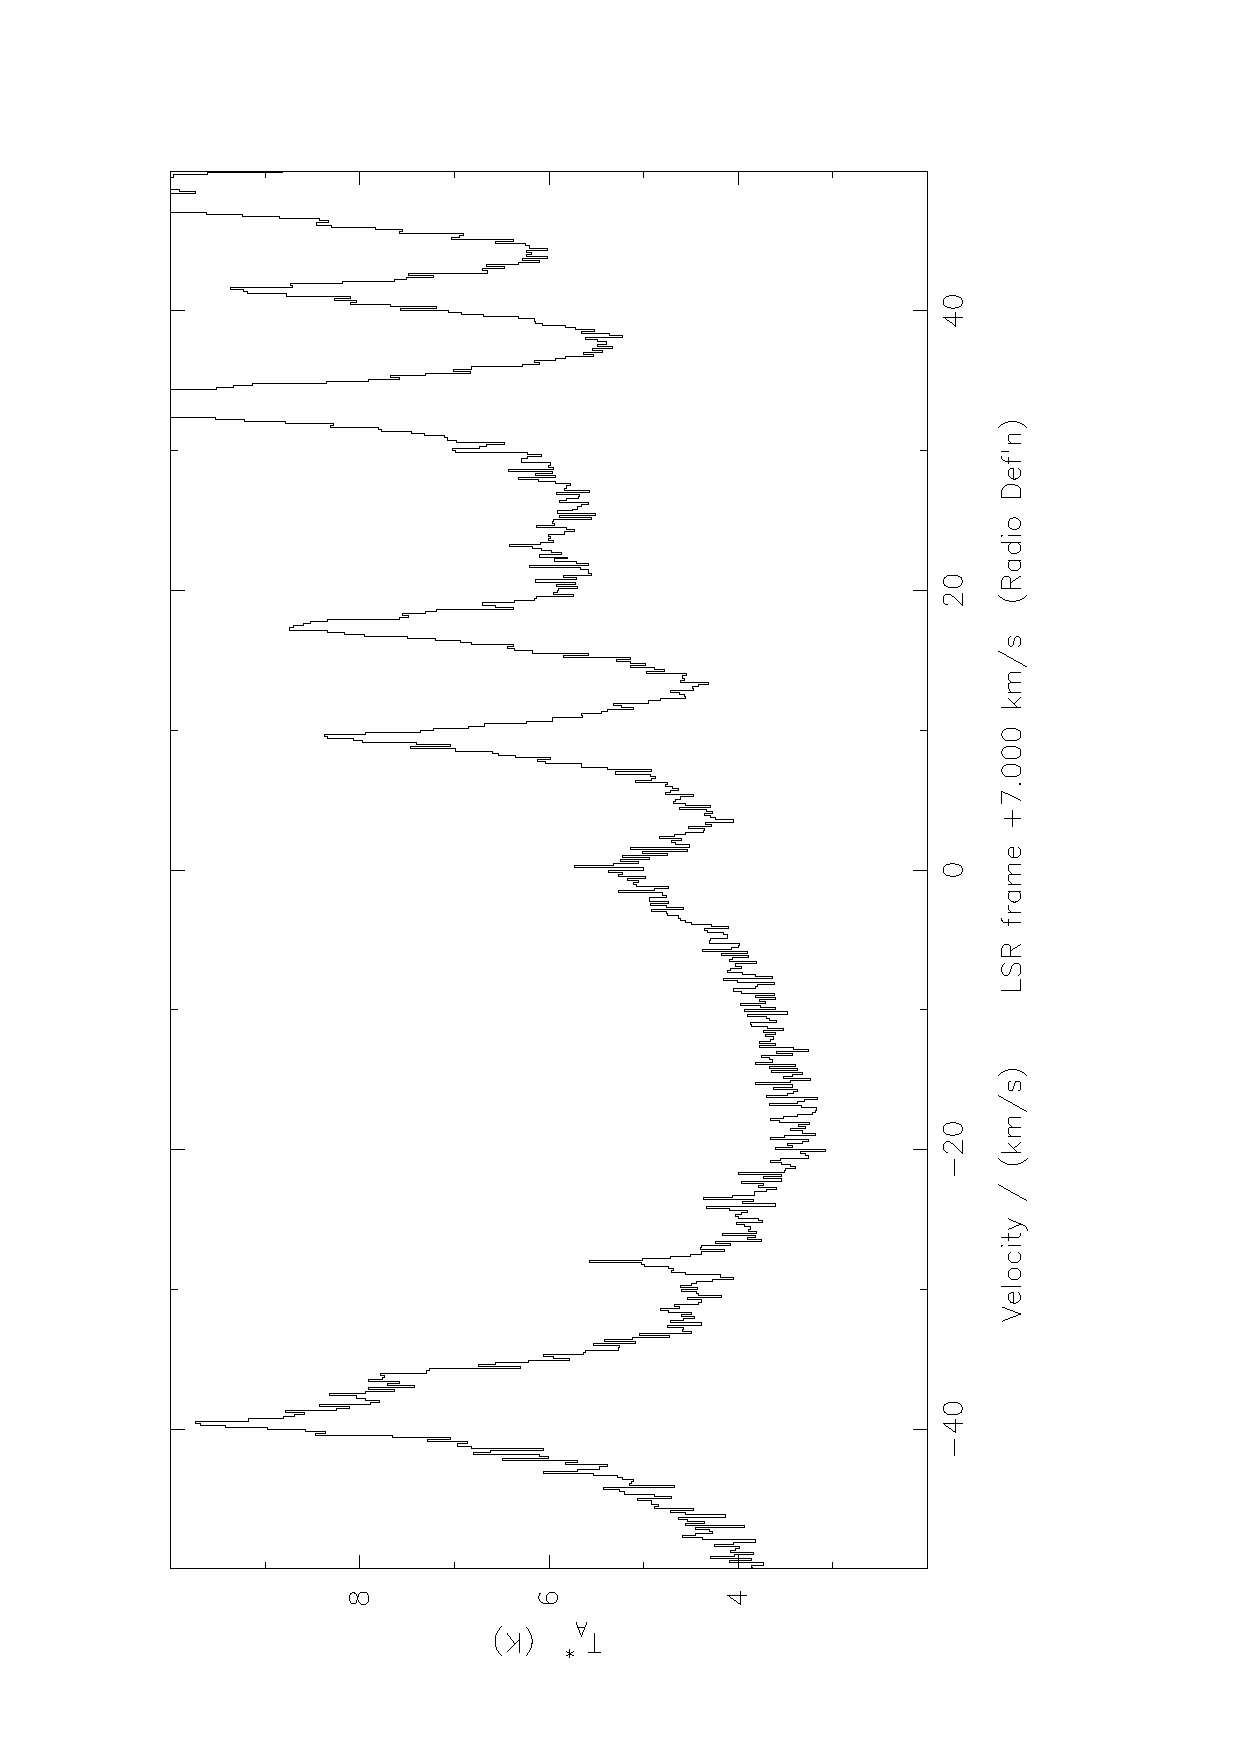
\includegraphics[width=0.8\textwidth]{sc8_hdo-usb}
\caption[Part of the same in the USB]
{\small{Figure~\ref{fig:set-x-orig} after changing to a frequency
x-axis and providing \SPECX\ with the correct lsr velocity, and
frequency in the upper sideband.
}}
\label{fig:set-to-usb}
\end{figure}

Here we see that our line is centered at about 0 km/s, because we have
referred the scale to an LSR velocity of 7 km/s, the actual velocity of
this source.

Once again, note that although the correct LSR velocity was chosen
when the observations were made, as seen in the `header' below the
plot, this is largely irrelevant to this discussion. We can choose to
concentrate on any line by a correct choice of rest frequency,
sideband and velocity.

For an equivalent display of the \textit{lower sideband} line we need to
change the sideband also:
\begin{terminalv}
 >> s-l-r-f 310.5333
 >> s-v-f \y\lsr\rad\7.0\
 >> ch-sid

 Warning ** Rest frequency set using values from SET-LINE-REST-FREQ.
 Do S-L-R-F. to use defaults from header

 Sector  1: First I.F. = -1.608541 GHz

  --- Header entries changed to other sideband ---
      Note that f_rest still refers to frequency
      used as reference in velocity transformation:
      You should not normally need to change this.

 >> s-p-sc
 Do you want automatic scaling of X-axis? (Y/N) [Y] n
 X-axis scale: Beginning and end? [ -50.00   50.00]
 Do you want automatic scaling of Y-axis? (Y/N) [N]
 Y-axis scale: Beginning and end? [   2.00   10.00]
 >>
\end{terminalv}


Note that \texttt{ch-sid} turns on the default x-axis scaling, and we
have to reset this.  Then we get the plot in Fig.~\ref{fig:set-to-lsb},
containing the other HDO line, again centered around 0 km/s:

\begin{figure}[ht]
\centering
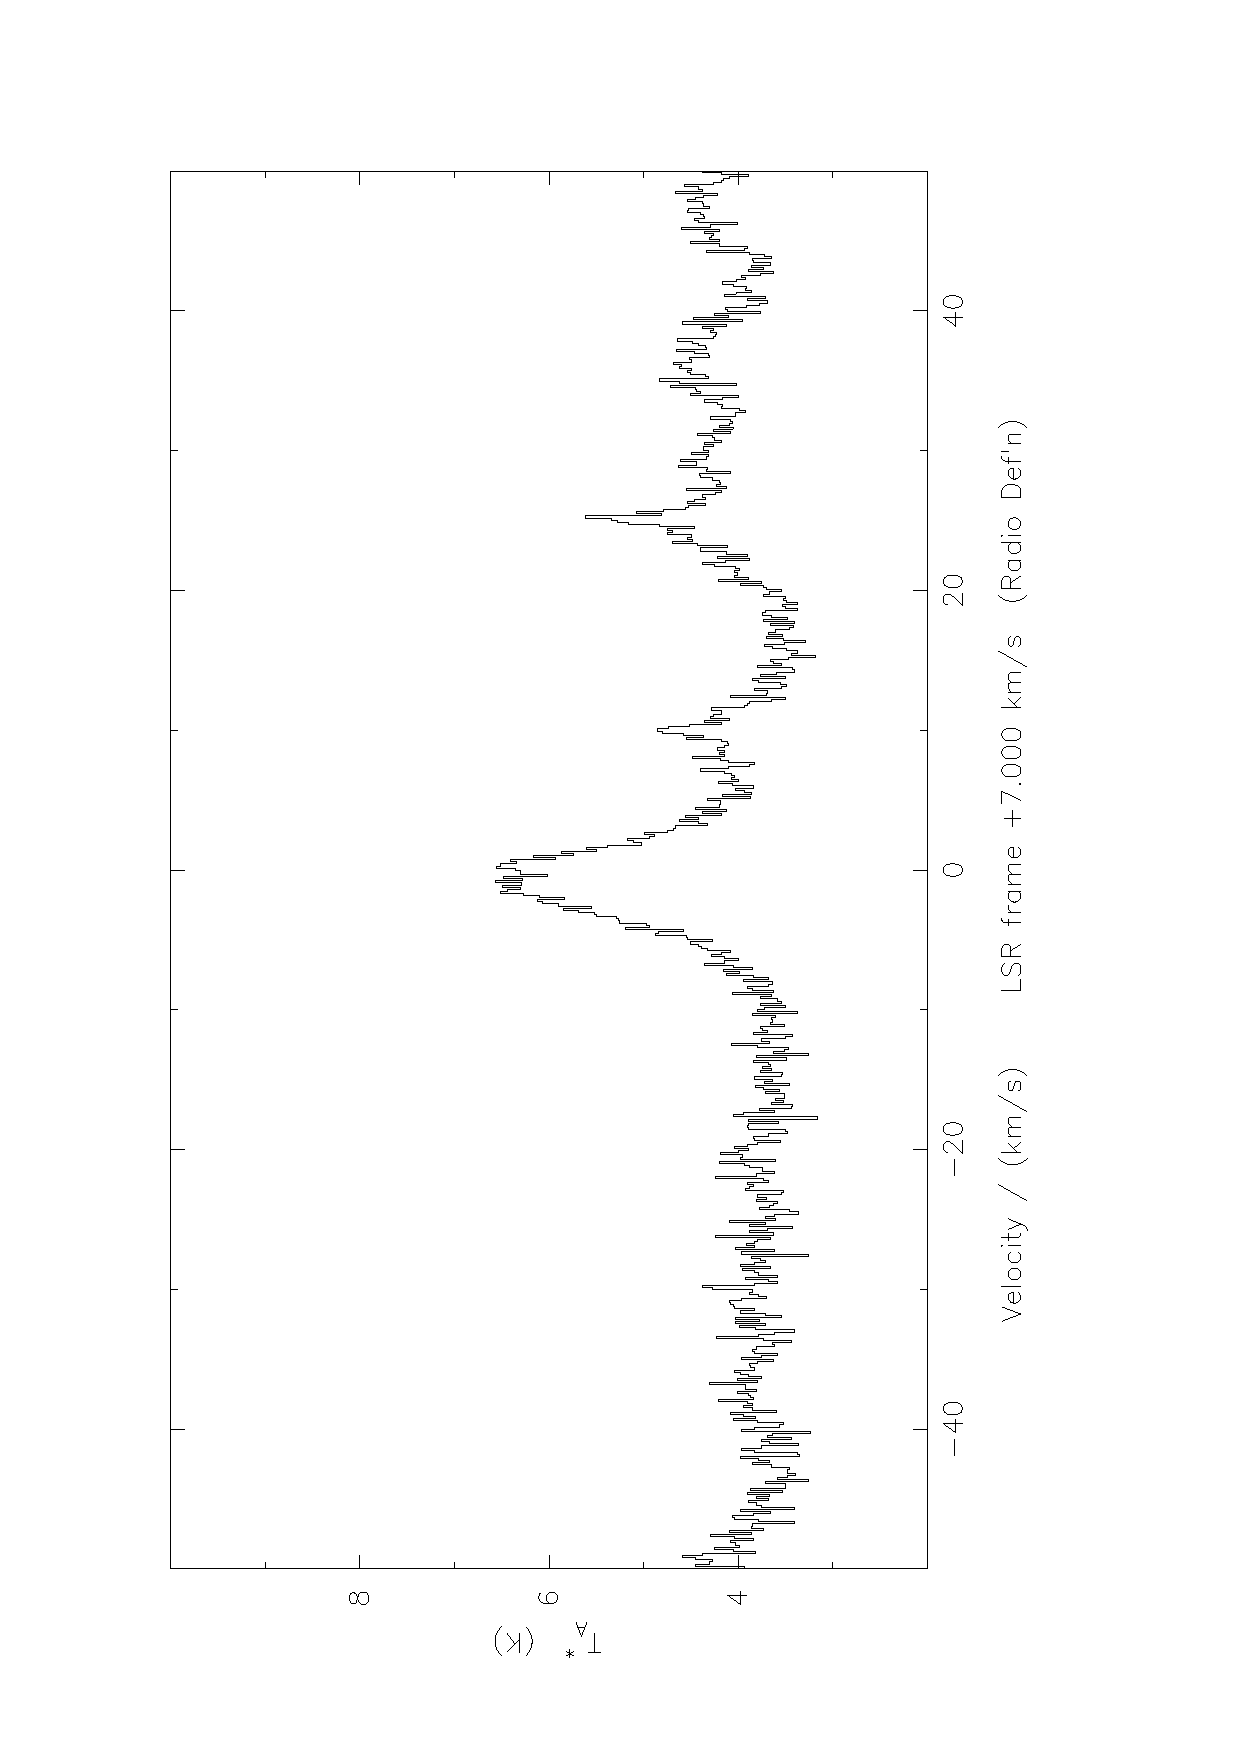
\includegraphics[width=0.8\textwidth]{sc8_hdo-lsb}
\caption[Part of the same in the LSB ]
{\small{Figure~\ref{fig:set-x-orig} after changing to a frequency
x-axis and providing \SPECX\ with the correct lsr velocity, and the
frequency in the lower sideband.
}}
\label{fig:set-to-lsb}
\end{figure}

Sometimes, because it's fairly difficult to get everything the way one
might want it, it can be useful to collect the commands together in a
procedure, which can be edited and re-run until you get the result you
want. For example, the following procedure plot three lines which
happen to appear in the same spectrum on a common velocity axis. Two
of the lines are in the lower sideband, and one in the upper
sideband.\footnote{By the way, in case I didn't mention it before
any characters following a `{\tt{!}}' on a command line are taken to be
comments. I often use comment lines to `store' command lines I might need
some other time.}

\begin{terminalv}
!o-fil tests
rea-sp 1 1
s-l-r-f 362.6303
ch-sid
s-v-f\y\lsr\rad\0\
s-p-sc\n\-10 30\n\-2 15\
n
!
rea-sp 1 1
s-l-r-f 362.7359
ch-sid
s-v-f\y\lsr\rad\0\
s-p-sc\n\-10 30\n\-2 15\
off 5
over 1 3
!
rea-sp 1 1
s-l-r-f 365.3634
s-v-f\y\lsr\rad\0\
s-p-sc\n\-10 30\n\-2 15\
off 10
over 1 3
!
cl-pl
!the end
\end{terminalv}

The result of this procedure is shown in Figure~\ref{fig:s-l-r-f}.

\begin{figure}[htb]
\centering
\includegraphics[width=0.8\textwidth]{sc8_s-l-r-f}
\caption[Using s-l-r-f etc]
{\small{Bottom through top: lines of HNC (4--3; 362.3603~GHz), H$_2$CO
(5$_{05}$--4$_{04}$; 362.7359~GHz) and H$_2$CO (5$_{23}$--4$_{22}$;
365.3634~GHz) observed toward NGC2071IR; all three lines appear in the
same spectrum by virtue of the choice of receiver tuning frequency and
IF. The first two lines are in the lower sideband, and the
third line comes from the upper sideband. The latter is a fairly
high-excitation line (57~cm$^{-1}$) and thus is quite weak. Using a
combination of \texttt{s-l-r-f} and \texttt{ch-sid} as shown in the text it
is possible to plot all three lines on a common velocity scale.
}}
\label{fig:s-l-r-f}
\end{figure}



\subsection{Reduction of frequency-switched data}
\label{sec:fsw-reduction}

For observations taken in frequency-switched mode, the `raw' spectrum
consists of two copies of the line profile displaced in both plus and
minus frequency directions from the nominal line position by an amount
equal to the frequency switch employed. This situation is shown in the
top part (`original') of the schematic below. Here the nominal line
position (at the centre of the spectrometer window) is indicated by
`{\tt{+}}' and the frequency switch offset by `{\tt{fsw}}'. There is a
positive offset in the signal phase, and a negative one in the
reference phase. The spectrum thus has both positive- and
negative-going features (`{\tt{+L}}' and `{\tt{-L}}' respectively)
corresponding to the two phases.

The data reduction of such a spectrum is done by `shifting and
adding': copies of the spectrum are shifted in frequency by plus and
minus the frequency-switch amount, and then subtracted. The result is
divided by 2 to form the end result, as shown below schematically in Fig.~\ref{fig:fsw_schematic}.

\begin{figure}[ht]
\centering
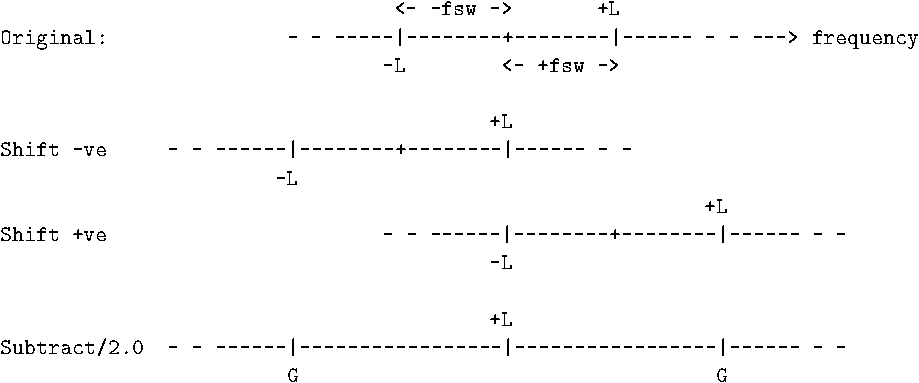
\includegraphics[width=0.9\textwidth]{sc8_fsw-fig}
\caption{Schematic -- how frequency-switched data is reduced}
\label{fig:fsw_schematic}
\end{figure}

The final spectrum consists of the line at the correct frequency (and
velocity) and two half-height negative `ghost' images of the line (at
`{\tt{G}}' in the plots above). The separation of the ghosts from the
line is $\pm2.0\Delta\nu$, where $\Delta\nu$ is the original
frequency-switch. Any offset and/or slope in the spectrum is
automatically removed by this step, but curved baselines are not. A
`real-life' example of the above process is shown in
Figure~\ref{fig:fsw_reduction}.

\begin{figure}[htb]
\centering
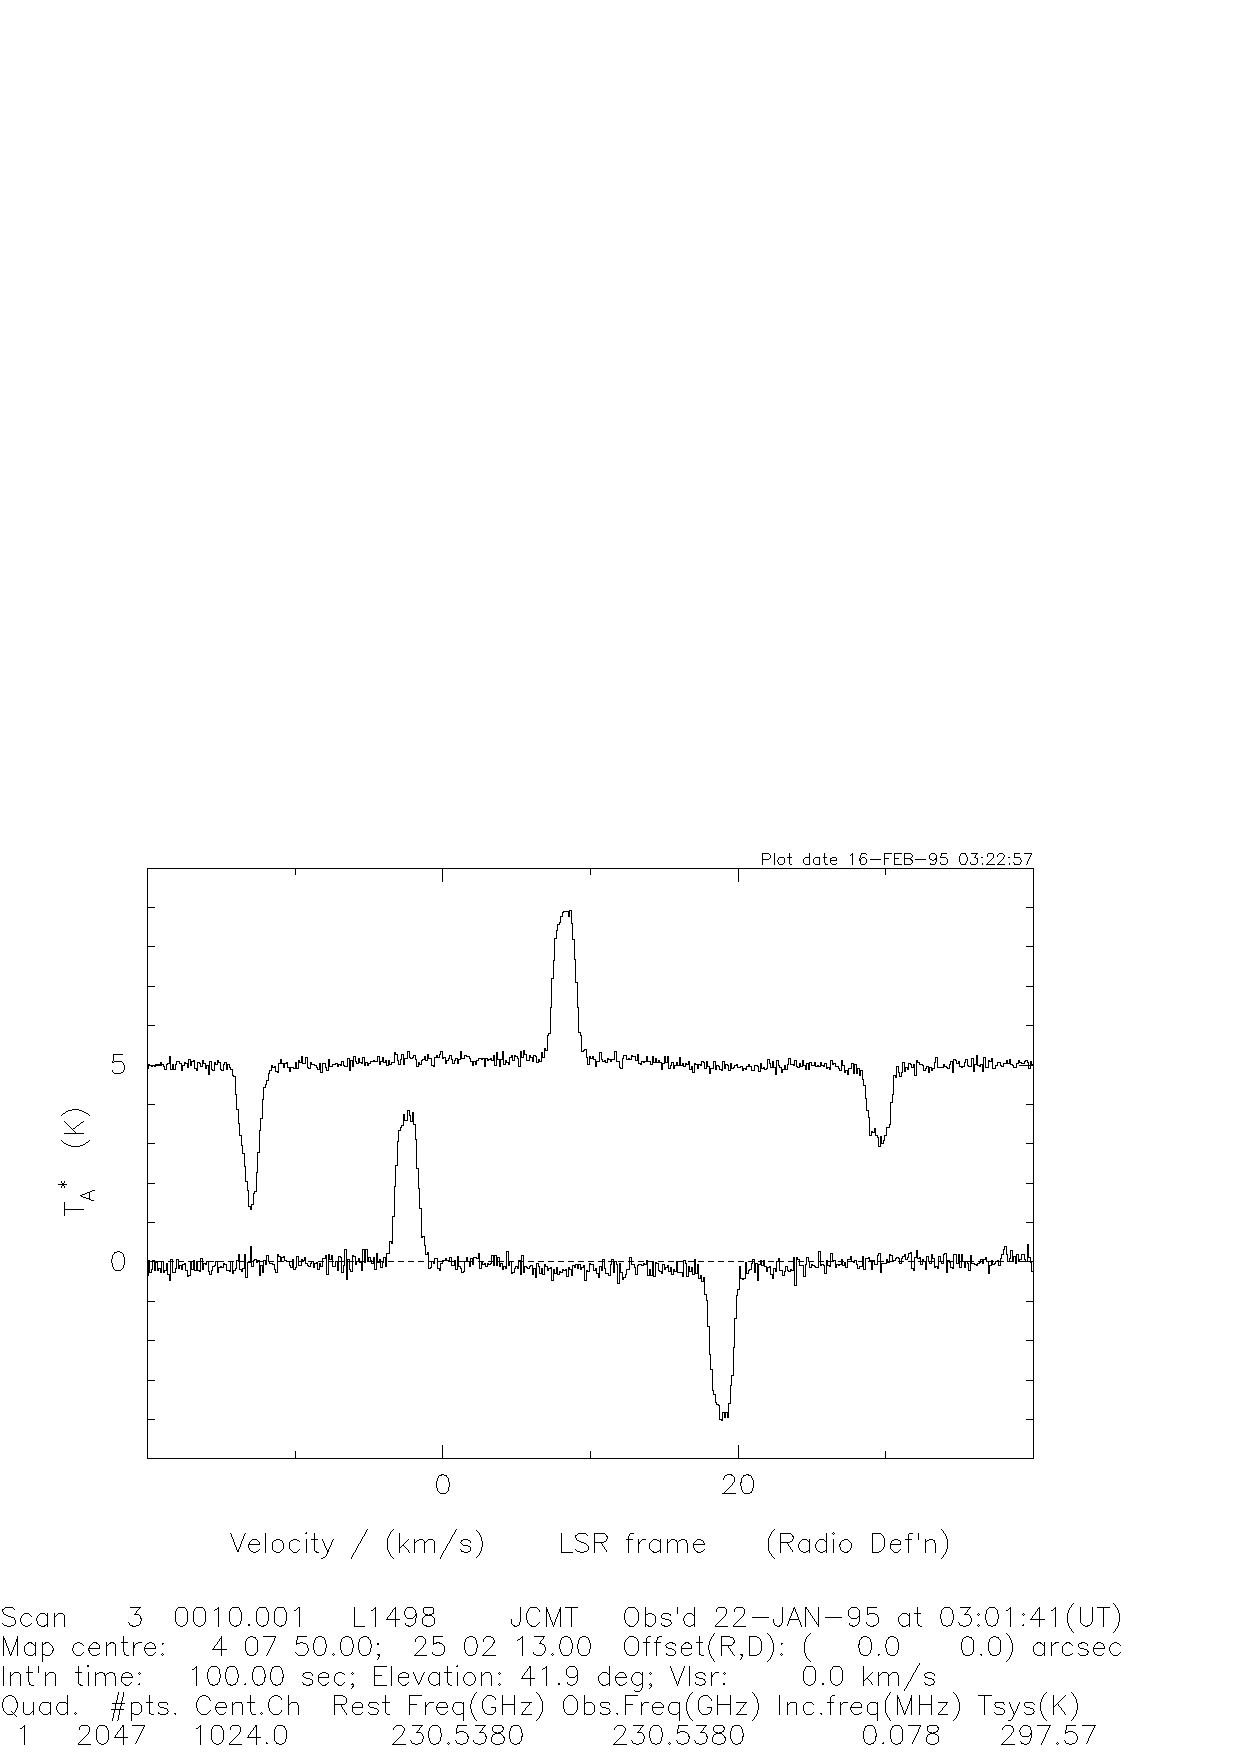
\includegraphics[width=0.8\textwidth]{sc8_fsw_reduction}
\caption[Reducing frequency-switched data]
{\small{A portion of the `raw' frequency-switched spectrum of the CO(2--1)
emission towards L1498 appears at the bottom of this panel. A linear baseline
was subtracted for clarity. At the top is the `shifted and subtracted'
spectrum. The final CO line profile is at the middle (V$\sim 8$ km/s), flanked
by negative-going `ghost' images. The left-hand one of the latter coincides
with a `ghost' image from telluric CO, off the frame to the left.
}}
\label{fig:fsw_reduction}
\end{figure}

In practice one can expect a slowly-varying (and sometime large
amplitude) sinewave across the band when observing in a
frequency-switched mode. It may therefore be necessary to subtract
higher-order polynomials from the baseline than with position- or
beam-switching. In addition strong interference spikes can appear in
the band, particularly when using A2. In other observing modes these
will be largely cancelled out, but in the frequency-switched mode any
such spike has the opportunity to appear twice. Such spikes may be
accompanied by `ringing' as a result of the Fourier transform applied
to the data by the DAS. These problems should be taken into account
during the data reduction.

Practical data reduction therefore consists of the following steps,
some of which may be optional:
\begin{itemize}
\item
Average all equivalent spectra together.
\item
If using more than one subband with the \das\ merge the subbands
together using the \SPECX\ command \texttt{das-merge}. This step will not
be needed if the spectra are taken with the \aosc .
\item
Apply Hanning smoothing to the spectrum if there is clear `ringing'
associated with spikes in the band.
\item
Remove interference spikes using \eg\ \texttt{rem-spike} or \texttt{set-chann} in {\SPECX}.
\item
There is a special procedure ({\tt{fsw}}) to do the shifting and
adding; it needs to be provided with the frequency shift you used
during the observing; \eg\ type:

\SP\ \verb|fsw 8.1|

In this case the frequency switch was $\pm8.1$~MHz.

This takes the contents of the x-register (assumed here to be the
result of the previous steps listed above) and replaces it with the
shifted-and-averaged version. As noted within the procedure you may be
asked to provide a frequency; this is the result of a software
workaround for `slow-frequency switching' (using receivers A2 and
C2). To find out the frequency run \texttt{SPECSUM} and note the rest
frequency given there for the data in question.

\item
Any residual baselines can now be removed with a polynomial (use \texttt{f-p-b} in {\SPECX}) or composite (polynomial and sinusoidal; use \texttt{f-c-b}) function.
\item
Save the final result, once you are happy; you won't want to do all
this again.
\end{itemize}



\subsection{Hardcopy and file output}
\label{sec:specx_12}
If you really want to impress the tourists with your data you should
plot out some spectra, or better still, maps, on the laserprinter, or make
GIF files for WWW
display.  There are two ways to do this.

For spectra the easy way is to use the command \texttt{laser}.  This command
creates
a plot file which may be sent to the local laser printer (defined in the
setup of the node you are working at).  The command \texttt{see-plot} has
a similar effect to \texttt{laser}. In this case you provide the output
device (terminal, printer, or null --- the latter is a bit bucket);
\eg :

\begin{terminalv}
 >> see-plot
 Terminal / Hardcopy / Null (T/H/N) t
 -- sxgdevice --/xwindow         SPECXDIR:SPECX_PGPLOT.PS
 >>
\end{terminalv}

A more involved way involves first creating a plot file with which you
can then do whatever you want. In this case first select the output
medium you want using the command \texttt{s-h-d}:

\begin{terminalv}
 >> s-h-d
 Printers available:
 cps_l,            cps_p,            ps_l,             ps_p,
 ln03_l,           ln03_p,           ecpsf_ltex,       ecpsf_ptex,
 epsf_ltex,        epsf_ptex,        gif_l,            gif_p

 Printer type? [gif_l] cps_l
 >>
\end{terminalv}

As you can see there are quite a few possibilities, thanks to the use
of up-to-date PGPLOT. In this case I wanted to change from a landscape
GIF format to a color Postscript landscape plot. \SPECX\ always gives
the output file a default name; \verb|specx_pgplot.ps| for Postscript,
\verb|specx_pgplot.eps| for Encapsulated Postscript,
and \verb|specx_pgplot.gif| for GIF files, for instance. Unix being
what it is, this file will be overwritten every time you create a new
plot file of the same type.  Therefore if you want to save the plot
file, rather than have it overwritten when you make the next plot, you
should copy the generic file to a name of your choice; \eg :

\SP\ \verb|$ cp specx_pgplot.ps| \textit{myplotfile}\texttt{.ps}

% $ Help emacs

One cannot use the \texttt{laser} command for maps (see below).

\subsection{Making Maps}
\label{sec:specx_13}
Map making with \SPECX\ is straightforward but it can be tedious if
the map is quite large.  It would be best if you tried using the
following commands on a small map so that you get the idea and then
use repetitive command files to create the large maps.  Also, after
you have made a map you can't alter all the spectra in it without
pulling them out, working on them and then replacing them.  So if you
want all the spectra smoothed or binned or whatever, make sure you do
it before you make the map or you will have a job ahead of you. If
this happens to you, it would probably be faster to just re-make the
map.

\subsubsection{Getting The Parameters Right}
\label{sec:specx_13.1}
To make maps you have to create a map file first.  Then you put
spectra into the file.  Map files are similar to data files except
they always have read/write access.  The command to start a map file
is \texttt{open-map-file}.

Some words of advice first:
\begin{itemize}
\item
You will need to provide the number of points in each spectrum (they
should all be the same), which means you need to know this and have it
set to a sensible number before you get going in a production
mode. The number of points is given on a \texttt{laser} plot at the
extreme lower left, and if you use the command \texttt{print-spectrum-header} ({\tt{p-s-h}} will do) you can see the same
information. Once you set the number of points in the map set-up, it
will not be possible to stuff a spectrum containing fewer (if, say,
you smoothed the data first) or more points into that map.
\item
The number of points selected is a crucial item as far as memory and
disk space goes also. It is wise to limit the amount of the spectrum
you want in your map to as few channels (200 or fewer may be enough
sometimes) as is practical. Otherwise you may run out of disk
space. With the large maps which can be made using the \texttt{raster}
mode this is an important point. Limit the number of channels in the
spectrum using the \texttt{drop-channels} command. See below.
\item
Only one map can be open at any one time. This means that it is \textit{very} inefficient to transfer data from one map to another, using the
commands
\verb|get-spectrum-from-map| and \texttt{add-to-map} in a command file. It is
much better to hold the data in a \SPECX\ data file and use that as an
intermediary.
\end{itemize}

The key to all this is to experiment first with the data you plan to
put in a map. Let's illustrate this with an example of a real life
situation.

The first thing to do is open a map file. The following dialog ensues once we
type the command \texttt{open-map-file}:

\begin{terminalv}
>> o-map
File name? (extension will be .MAP) [    ] s140_core

Inquiring about file: s140_core.MAP
Map file does not exist: open a new one? (Y/N) [N] y
File title? S140_core_data
File owner? Robert_Simon
Set map centre automatically from first scan added to map? (Y/N) [Y] y
x (R.A.) & y (Dec) cell sizes? (arcsec) [  0.0   0.0] 6 6
Position angle of map y-axis? (degrees) [   0.0]
Maximum number of cells on x & y axes? [  0   0] 15 13
Number of spectral channels in map? 247

Map centre (i.e. pos'n corresponding to centre pixel)
will be the map centre of first spectrum ADDed to the
map after it is created. Use ED-S-H on first spectrum
if you want to force some other map centre.

>>
\end{terminalv}

Some explanation of the exchange is given below:
\begin{itemize}
\item
On issuing the \texttt{open-map} command and a filename, one is prompted
for a number of inputs if the map doesn't already exist (if it does,
that's the end of the conversation, and the map is just opened with no
further fuss).
\item
You give a map title and owner (note that these strings, like the ones
associated with data files, should not contain spaces, etc).
\item
Next you specify whether the map centre is determined automatically
from the first spectrum added to the map (this does not have to be the
central point); if you answer negatively then you can provide a
different central position. In the latter case note that the new map
centre should be as closely as possible an integral number of pixels
from the original observation centre in both coordinates.
\item
Next give the cell spacing and angle; these will probably be the same
as those used during the observations. However, you could make the
cell spacing half size, say, if you might want to fill in a sparse
grid with more points later.
\item
Give the map size in numbers of the above map cells in both
dimensions. Usually it is useful to choose a map size a little larger
than the actual map. You might want to expand it later with more
observations at the edges.
\item
Lastly, provide the number of channels in each spectrum. In this
example I happen to know that I will want 247 points, having done
some experiments beforehand. The baselines were a bit wiggly, so in
this case I was more interested in fitting only part of the baseline,
rather than saving disk space.
\end{itemize}

\subsubsection{Map Files}
\label{sec:specx_13.2}
To get data into the map, the command is \texttt{add-to-map}.  This takes
the spectrum in the \texttt{X} register and puts it in the map at the
correct cell position.  The first point you put in defines where the
map centre will be (using the source coordinates and offsets), if you
left that to be defaulted when you defined the map file setup with
\texttt{o-map}; hence it doesn't matter which map point you first put in
the map. There is also a \texttt{delete-from-map}
for removing data from the map.  If you want to see a listing of what is
in the map do \texttt{list-map}. If you want to take a spectrum out of a
map to look at it or to do some other operation on it, use \texttt{get-spectrum-from-map}.  And if you have gaps in your map, you can do
\texttt{interpolate-map} and \SPECX\ will try to fill in the holes.

So, here is the command file I used to add the spectra into the above
map file:

\begin{terminalv}
! map s140_core
do n 1 143
r-g-d\17\n\
r-g-d\18\n\;ave
r-g-d\19\n\;ave
r-g-d\21\n\;ave
r-g-d\22\n\;ave
r-g-d\23\n\;ave
r-g-d\24\n\;ave
das-merge\#\n\
drop 1190 220
f-p-b\-170 -150\-130 -110\^D\2\;sub
a-t-m
enddo
\end{terminalv}

In this case the map was made in the \texttt{raster} `on-the-fly'
mode. Because the integration time is limited to a few seconds in this
case, the integration time per point was built up by making the same
map 7 times, with calibrations before each scan, and a pointing part
way through the series of maps. Hence I ended up with observations 17
thru 19 and 21 thru 24 inclusive. Each one consisted of 143 spectra
(on a grid of 13 by 11 points). Hence the `do loop' runs through each
map point (143 times) (a) averaging the appropriate subscans together,
(b) merging the subbands together, (c) chopping off the unused part of
the spectrum, (d) fitting a quadratic baseline, and (e) adding the
result to the map. To save time the screen display was not turned
on. One can also do this kind of operation effectively with the \texttt{read-gsd-raster} and \texttt{merge-files} commands -- see
Section~\ref{sec:r-g-r}.

This file illustrates some more points about command file syntax.
\begin{itemize}
\item
Comment lines can be inserted by starting the lines with \texttt{!}.
\item
The `{\tt{n}}' in the \texttt{das-merge} command inhibits subband offset
adjustments; the `\verb|#|' is a `placeholder' for the default channel
drop.
\item
Two regions are chosen either side of the line emission for the
polynomial fit.  Note the method, using \verb|^D| (or \verb|^Z|), of
terminating
input to questions which have a larger number of possible answers
than you need.
\end{itemize}

You may well find yourself wanting to replace all or part of your map
subsequently. \SPECX\ can be told to allow this, or not, using the
\texttt{set-map-access} command. Thus:
\begin{terminalv}
>> s-m-a
Replace existing map spectra? (Y/N) [N] y
Maximum distance (pixels) from nearest gridpt? [   0.3]
..
\end{terminalv}
Note that it is possible to set the positional tolerance of grid
positions versus observed positions. The default is 0.7 pixel, but I
prefer it tighter than that.

\subsubsection{Dealing with lines in the other sideband}
\label{sec:other-sideband-maps}
Quite often it happens that one feels quite clever in having set up a
special frontend and \das\ configuration in order to observe two or
more lines in both sidebands simultaneously. That is the easy part;
dealing with the data reduction, especially making a map of the
line(s) in the other sideband requires a knowledge of the information
in Section~\ref{sec:modifying-axes}. As an example of the application
of this, the following map-making file is offered as an example of how
to make a map of CS 7--6 in the lower sideband, having observed CO
3--2 in the upper sideband. Various lines have been commented out, but
can be brought into service as required:
\begin{terminalv}
! map-adding procedure
! CS 7-6
!
declare scan i4
declare first i4
declare last i4
ask 'scan?' scan ?
ask 'first subscan?' first ?
ask 'last subscan?' last ?
do n first last
s-l-r-f 0 0 0 0
r-g-d \scan\n\
das-merge\#\n\
change-sideband
s-l-r-f 342.8833
set-int n
! decent baselines:
r-l-b\-55 -35\30 70\
! poor baselines
!f-p-b\-80 -40\-26 0\^Z\3\;sub
drop 100 1000
! n
a-t-m
enddo
\end{terminalv}

\subsubsection{The \texttt{read-gsd-raster} routine}
\label{sec:r-g-r}
Because map making can be slow due to system overheads, it is quite
often useful to create a basic data file first from the various map
observation GSD files. The routine \texttt{read-gsd-raster} provides this
capability. You should have a file open first, to which the data can
be written, and the routine reminds you to turn off the screen chatter
with \verb|>> s-l-f n| if you don't want to see all the gory details.

Then, for example, the routine looks like this:

\begin{terminalv}
>> r-g-r
 GSD scan number? [ 337] 333
 GSD version  5.3

 Use SET-LIST-FILE N to reduce output messages

 File number? (EOF to list) [1]
 1  junk                                      W    -1
 File number? (EOF to list) [1]
          (x,y) offset = ( -56.0, -56.0) arcsec
          rotation angles: x2y =  -90.0 deg.; v2y =    0.0 deg.
          (r,d) offset = ( -56.0, -56.0) arcsec


 Stack posn    Scan no    Title
     X          333      0333.0001   IRAS2227 JCMT

 Perform DAS-MERGE before writing ? (Y/N) [Y]
There are  222 overlapping channels
 Number of overlap channels to use? [ 111]
 Adjust any DC offset quadrants? (Y/N) [N]

\end{terminalv}

Then, away it goes. This routine does not fit baselines or truncate
the noisy channels from the ends of the spectra, but it
does \texttt{das-merge} the spectra as required. Subsequent application
of the command \texttt{merge-files} allows data which should go in a
single map cube to be combined. If one has two files containing
grid, pattern, or raster data taken to a common centre \texttt{merge-files} will combine these data in a third file, averaging data
taken at the same offsets. Thus this method is especially useful when
one has data taken by several observers who have been confused about
exactly where they should be observing, or when one has several
observations of the same map grid. With the recent upgrade in speed
resulting from improvements to the \texttt{r-g-d} routine this method
does not confer any special advantage as to speed of application. It
also tend to gobble up disk space due to the possibility of creating
several large files rather than one.

\subsubsection{Grid Spectra}
\label{sec:specx_13.3}
One of the most useful ways of displaying small \SPECX\ does maps is
called \texttt{grid-spectra}. This produces postage-stamp size spectra on
the screen lined up in the order they appear in the map.
Figure~\ref{fig:specx_fig6} shows what happened when I gave the
following commands:

\begin{terminalv}
>> gr-sp
X-axis range in Velo? (km/s  ) [  215.000,  245.000] -160 -130
Y-axis range in Kelvins? [   -5.000,   20.000] -2 6
Also plot interpolated spectra? (Y/N) [N]
R.A. offset scaled from   36.000 to  -36.000
Dec. offset scaled from   24.000 to  -36.000
..
>
\end{terminalv}

\begin{figure}[htb]
\centering
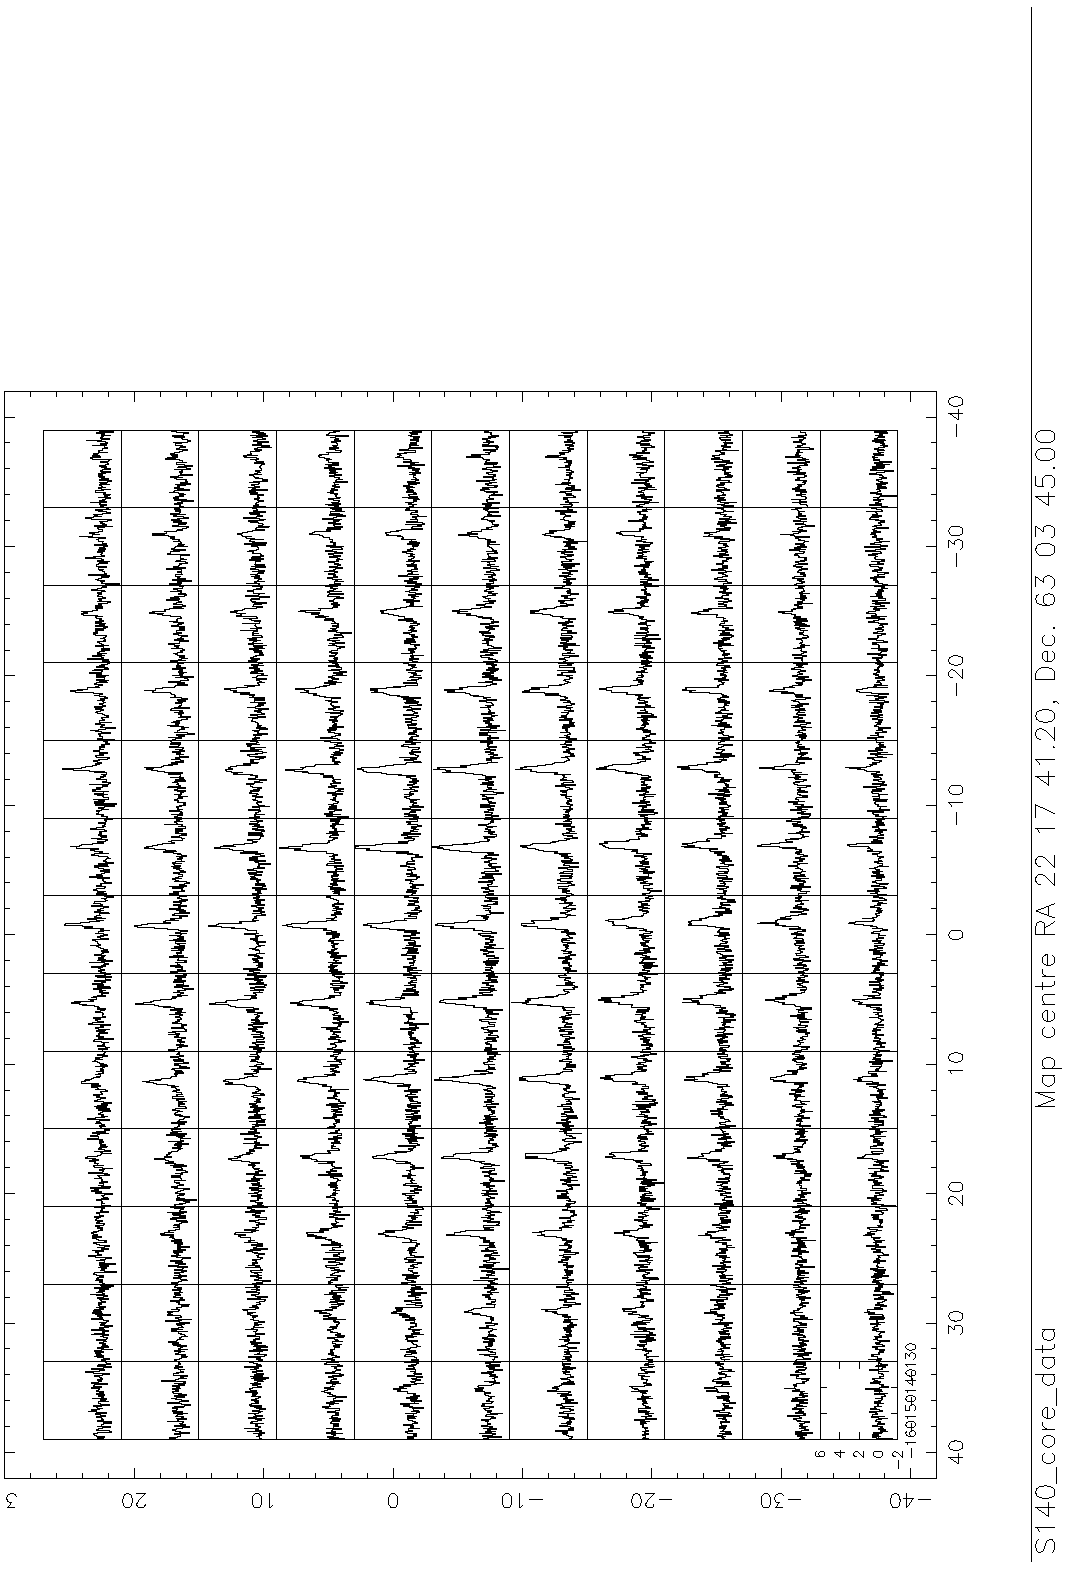
\includegraphics[width=\textwidth]{sc8_gr_sp}
\caption[`Postage-stamp' (grid) spectrum plot]
{\small{Using the \texttt{grid-spectrum} command.}
}
\label{fig:specx_fig6}
\end{figure}

If the spectra does not come out right on the screen, try
experimenting with \texttt{set-map-size} and \texttt{set-map-scales}.  The
map size determines the size of the window on the screen and the map
scale determines what is in the window.

\subsubsection{Contour Plots}
\label{sec:specx_13.4}
Making contour plots with \SPECX\ is easy.  The command is \texttt{contour-map}.  Figure~\ref{fig:specx_fig7} shows the result of the
following commands on the map that is in Figure~\ref{fig:specx_fig6}.

\begin{terminalv}
>> cont
Velo range? (km/s  ) [-160.0000,-130.0000] -142 -139
Integrated intensity? (rather than average) (Y/N) [Y]
R.A. offset scaled from   36.000 to  -36.000
Dec. offset scaled from   24.000 to  -36.000
\end{terminalv}

\begin{figure}[htb]
\centering
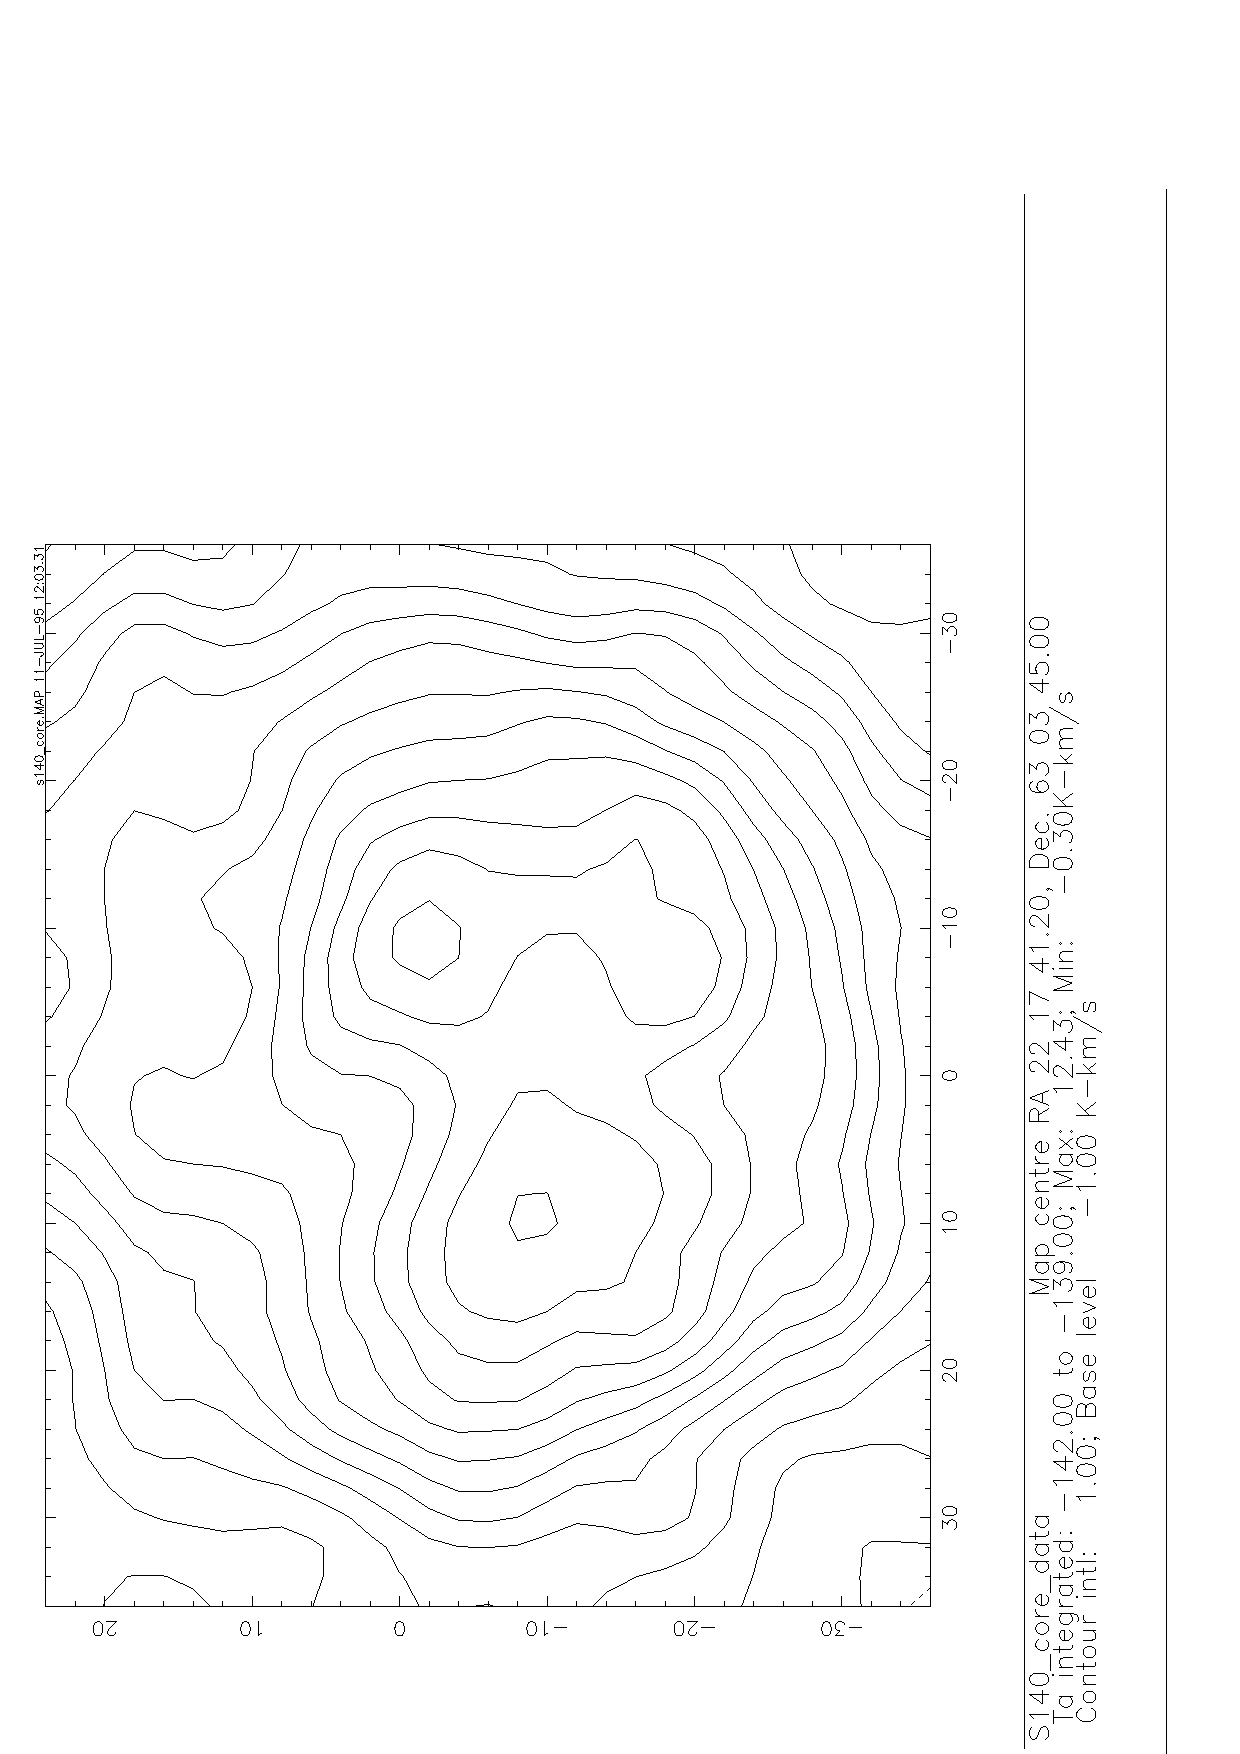
\includegraphics[width=0.8\textwidth]{sc8_cont}
\caption[Contour plot example]
{\small{Contour plot of integrated emission over the line centre made
using \texttt{contour-map}.}  }
\label{fig:specx_fig7}
\end{figure}

Again, if you have trouble getting what you want, adjust the map size
and scale.  Also, if you do \texttt{set-contour-levels} you can give it
specific levels by saying no to the question about `Auto-contouring
required'.

\subsubsection{Color `grayscale' images}
\label{sec:grayscale}
Contour plotting is a bit boring; you can liven up the results by
asking for grayscale plots using the command \texttt{grayscale-map}
({\tt{gray}} is enough)\footnote{In deference to British users, \texttt{grey} is an allowed alternative spelling for \texttt{gray} in the commands
in which it appears.}  Actually, most people make color `grayscale'
images these days; they are much more interesting. Thus:

\begin{terminalv}
>> gray
Velo range? (km/s  ) [-160.0000,-150.0000] -142 -139
Integrated intensity? (rather than average) (Y/N) [Y]
R.A. offset scaled from   36.000 to  -36.000
Dec. offset scaled from   24.000 to  -36.000
 -- scale_bar --
    greyscale limits:  -0.3037275       12.43124
    plot limits:         25.00000       140.7970       40.00000
  136.4975
    device size:         220.0516       144.4975
    nx and ny:                   1           1
Setting colour table 1: linear grey scale
\end{terminalv}

This will produce a grayscale plot with overlaid contours. If you want
to get rid of the contours, use \texttt{set-gray}, and answer `\texttt{n}'
in response to the query about contours:

\begin{terminalv}
>> set-gray
Set greyscales automatically? (Y/N) [Y]
Overlay contours? (Y/N) [Y] n
Colour table? (greyscale=1) [ 4] 1
..
\end{terminalv}

The result is shown in Figure~\ref{fig:specx_gray}.

\begin{figure}[htb]
\centering
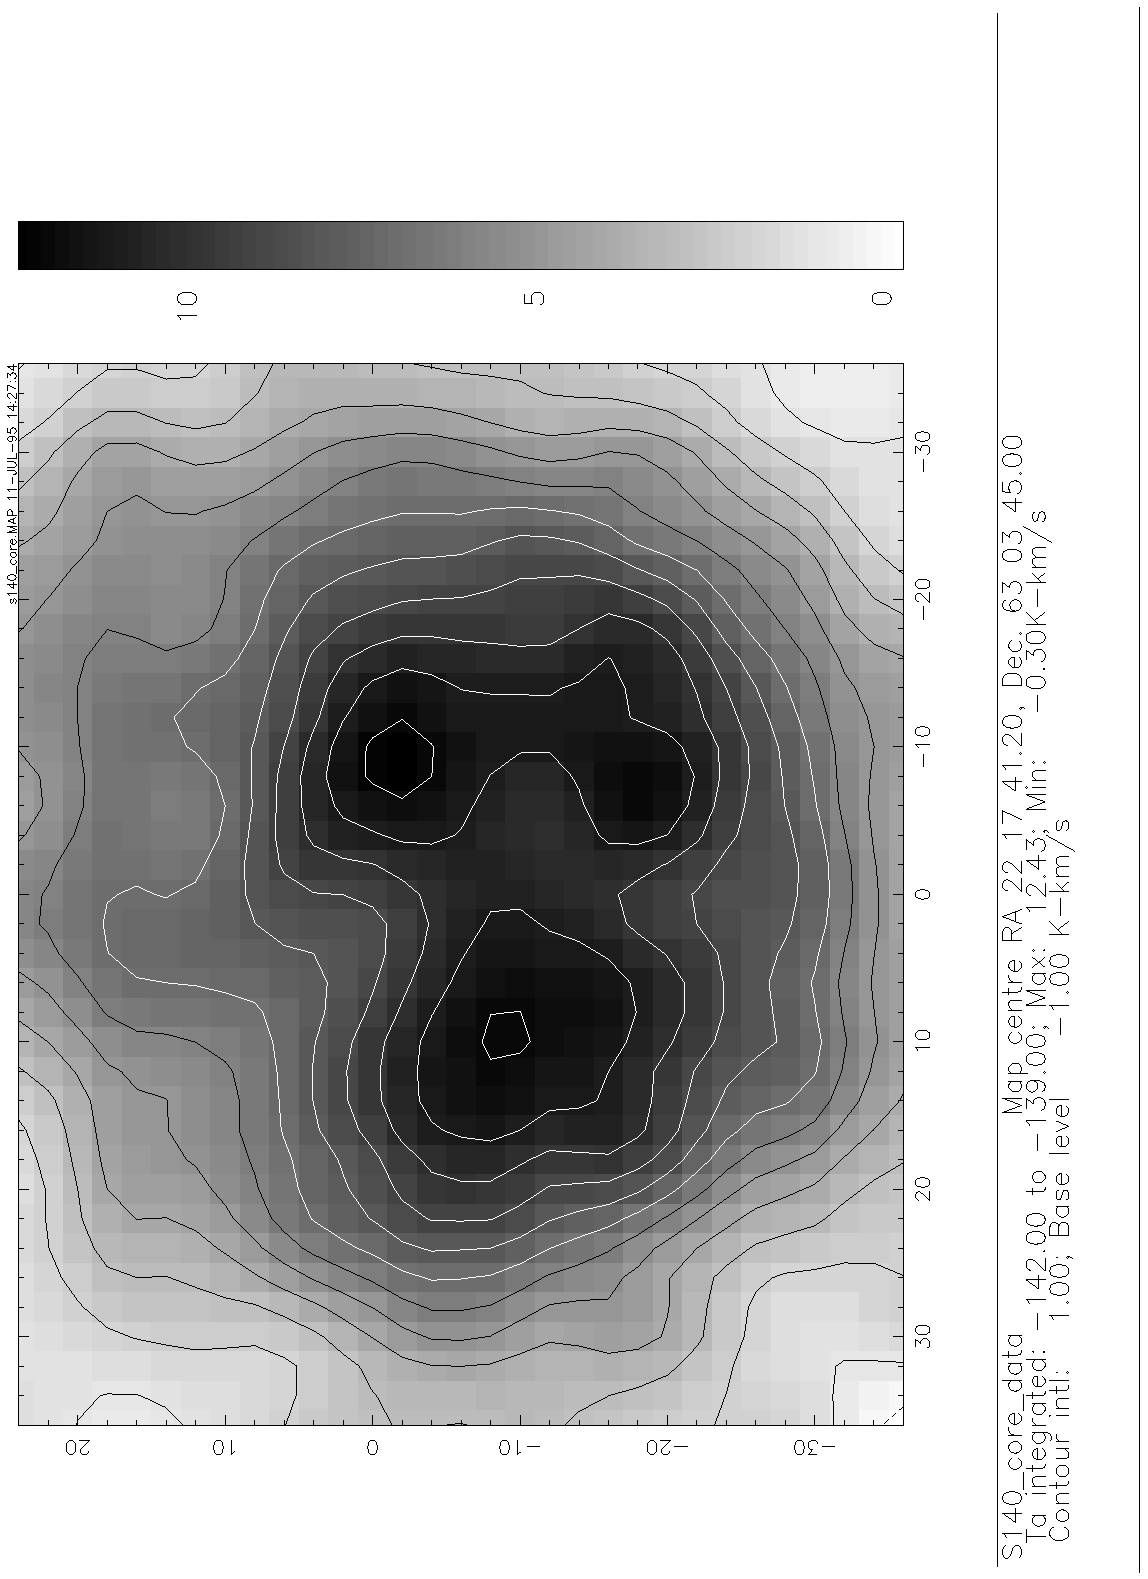
\includegraphics[width=\textwidth]{sc8_gray}
\caption[A gray-scale plot with contours]
{\small{Grayscale plot of the same field}
}
\label{fig:specx_gray}
\end{figure}

This really only works with a windowed terminal with a color
monitor. However, the color table referred to allows a number of
possibilities. Color table 4, for instance, produces a very nice blue
thru yellow `grayscale', and color table 5 is the ``Cambridge colour
spiral''. The best way to experiment with the option is to make a
grayscale plot in interactive mode.  Then, click on any point of the
display window and type `\texttt{h}' for `\texttt{help}'. A list of
interactive options will appear in your \SPECX\ window. \SPECX\ really
is very clever --- I suggest you experiment with the options.

Once you have a plot you like on the screen, you should save it, or at
least send it to the printer. To keep a recently made color Postscript
file, say, you might do the following:

\SP\ \verb|$ mv specx_pgplot.ps myplot.ps|\\
\SP\ \verb|$ lp -d color myplot.ps|

This would send it to a printer named 'color`.

\subsubsection{Channel Maps}
\label{sec:specx_13.5}
Another thing one can do is use \texttt{channel-maps} to make sequence of
maps of the integrated or average emission in successive velocity
slices.  Figure~\ref{fig:specx_chann_maps} shows the result I got from
the following:

\begin{terminalv}
>> chann
Velo range? (km/s  ) [-160.0000,-140.0000] -144.5 -136.5
Integrated intensity? (rather than average) (Y/N) [Y]
R.A. offset scaled from   36.000 to  -36.000
Dec. offset scaled from   24.000 to  -36.000
Channel width? (km/s  ) [     1.000]
Generating maps from cube - please be patient!
Maps now generated, going to contour them...
How many maps across page? (0=auto) [ 0] 4
Plotting on hardcopy device
 -- scale_bar --
    greyscale limits:   0.0000000E+00   6.000000
    plot limits:         25.00000       259.9995       40.00000
  137.9164
    device size:         264.9995       197.7896
    nx and ny:                   4           2
Setting colour table 1: linear grey scale
..
\end{terminalv}

The number of maps across the page can be chosen by you, but the auto
option often does a very presentable job. In this case I wanted eight
maps, four to a row.

\begin{figure}[htb]
\centering
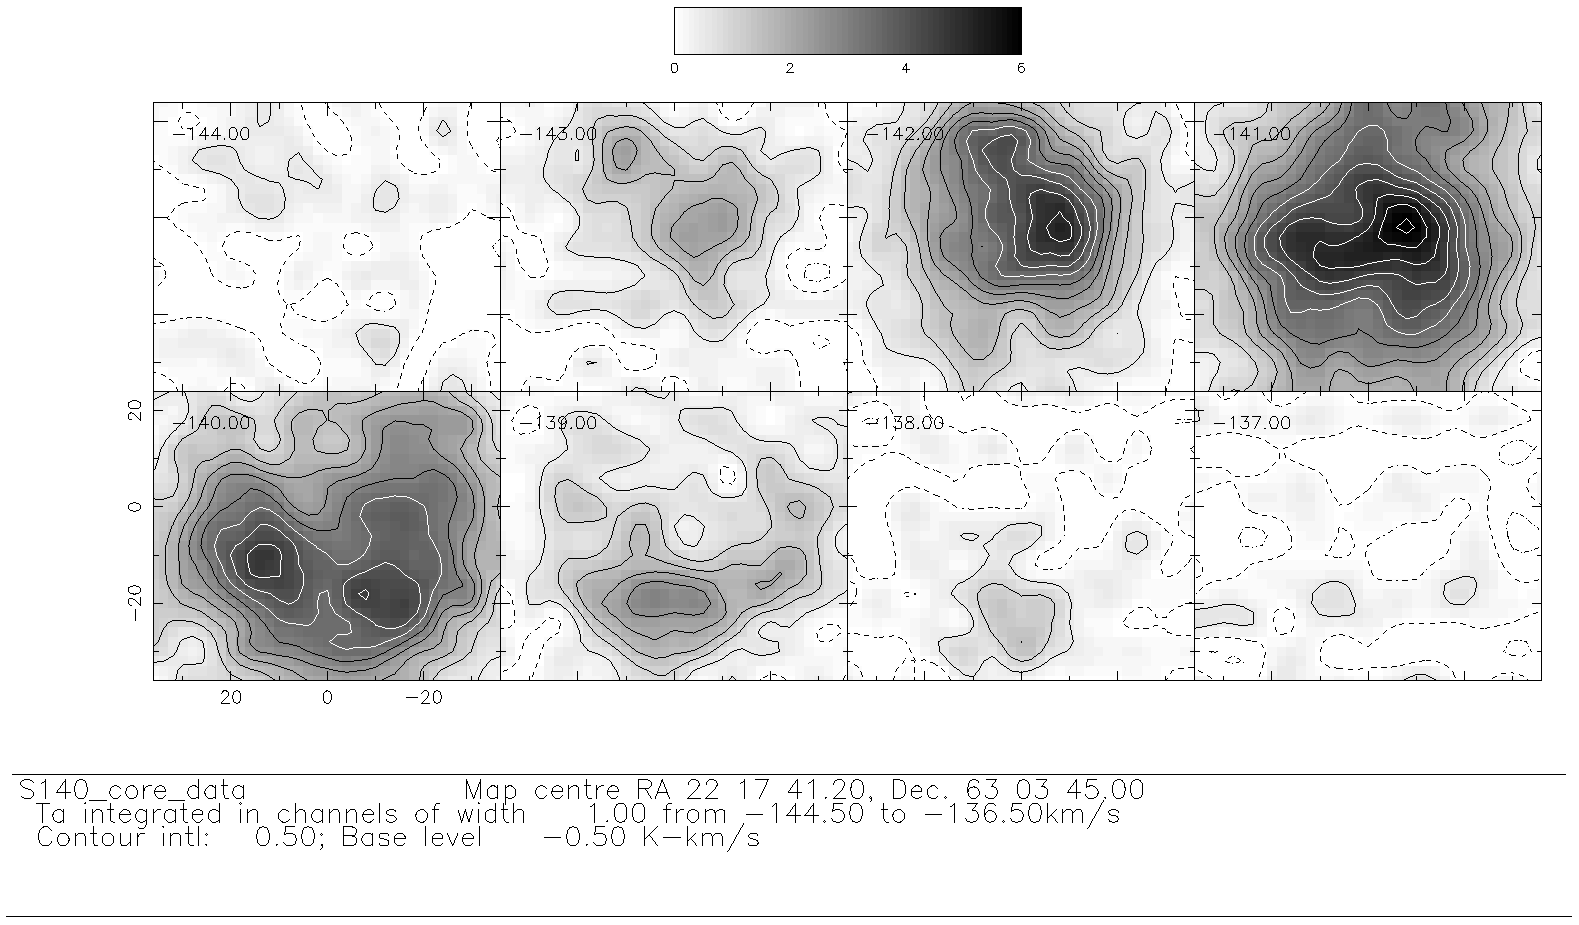
\includegraphics[width=\textwidth]{sc8_chann}
\caption[Velocity slices]
{\small{Output of the \texttt{channel-maps} command}
}
\label{fig:specx_chann_maps}
\end{figure}

Most of these map facilities are touchy and few people get the picture
they want the first time.  Experiment with them though, it's a good
way to pass the time at the summit.

\subsection{Data format conversion}
\label{sec:fits-etc}
As noted elsewhere the original spectral line data are written in \texttt{GSD} format. After processing by \SPECX\ the output data, both
spectrum datasets and maps, are in SDF format. For transmission to
other sites it is possible to convert the data to either \texttt{ASCII}
or FITS format via
\SPECX , if you don't want them in your native format.

\subsubsection{Conversion of older VMS \SPECX\ data to Unix-readable
format}
\label{sec:cvf_cvm}
Many people will have data reduced using the VMS versions of
\SPECX . These are in the wrong format to be read by Unix versions,
and it is necessary to convert them to the correct format. The
commands \texttt{convert-vax-file} and \texttt{convert-vax-map} are provided
for this purpose.
\begin{itemize}
\item
To convert a VMS \SPECX\ data file type \eg :
\begin{terminalv}
 >> c-v-f
 File name? ngc253.dat
\end{terminalv}
The new file will be named \texttt{ngc253.sdf} in this case.

Note that one needs to give the full name of the file ({\tt{ngc253.dat}}
in this case), otherwise the following very serious-looking error will
occur:

\begin{terminalv}
 >> c-v-f
 File name? ngc253
  --- openuf ---
      error in OPEN: FORTRAN i/o error #   1018
 Failed to open input file, IOSTAT =  1018
!! HDS locator invalid: value=' ', length=15 (possible programming error).
!  DAT_ANNUL: Error annulling an HDS locator.
 -- SPECX#010 -W- Error opening file --
 >>
\end{terminalv}
A similar error message will occur if the output filename already exists.
\item
Conversion of VMS maps (datacubes) proceeds along similar lines \eg :
\begin{terminalv}
 >> c-v-m
 File name? mars_12
\end{terminalv}

In this example, the input map name was \texttt{mars\_12.map}; the output
map name will be \texttt{mars\_12\_map.sdf}. Note however an inconsistency
with the \texttt{c-v-f} command: the full input map name is \textit{not}
required. Providing it will give an error \eg :

\begin{terminalv}
 >> c-v-m
 File name? mars_12.map
  --- openuf ---
      error in OPEN: FORTRAN i/o error #   1018
 Failed to open input file, IOSTAT =  1018
 File name was mars_12.map.map
 -- SPECX#010 -W- Error opening file --
 >>  3
\end{terminalv}
\end{itemize}

\subsubsection{Conversion to \texttt{ASCII} files}
\label{sec:specx2ascii}
If one wants to create a simple table of intensity versus the chosen
abscissa (obtained using \texttt{set-x}), say, for subsequent
manipulation using \texttt{PGPLOT} or \texttt{MONGO} this can be done using
the command

\SP \verb|write-ascii-spectrum|

({\tt{w-a-s}} will do). The header information is minimal.

\subsubsection{Conversion of single spectra to FITS format}
\label{sec:specx2fits}
To convert to a format readable by \texttt{CLASS}, it is first necessary
to generate spectra arrays continuous in velocity/frequency
space. Thus one must first have used the \dm\ feature of \SPECX\ for
all but single-subband data of the \texttt{DAS}. There are two ways of
doing this\footnote{The following is based on notes made by Remo
Tilanus}.
\begin{itemize}
\item
First write the spectra to a \SPECX\ output file after applying \dm\
and any other processing you want (such as baseline fits, binning
etc). Then use the
\SPECX\ command

\SP \verb|tofits|

This will ask four questions: (a) which \SPECX\ file number you want
to use (hence the file must be open and read-permitted), (b) whether
you want to use the original scan numbers or the sequence number in
the \SPECX\ file, and (c) the first and (d) the last scan in the input
file to be processed by \texttt{tofits}. If you have single-position
spectra (each with a distinctive integration number), or averages of
the same, then choosing the original scan number option would
probably be best. If your data are a sequence comprising a map, say, made with
the \texttt{grid}, \texttt{pattern} or \texttt{raster} observing commands, then
the scan numbers will be the same, but the subscan numbers will be
incremented. In this case either the sequence number or the
scan/subscan will do.

The output filename has the following pattern in case one selects the
option to imprint it with the original scan number:

\begin{terminalv}
jcmt_nnnn_xxx.fits
\end{terminalv}

where \texttt{nnnn} is the scan number and \texttt{xxx} the subscan
number. That is, the output file names might look like
\begin{terminalv}
     jcmt_0051_001.fits
     jcmt_0051_002.fits
            .
            .
            .
     jcmt_0051_015.fits
\end{terminalv}
in the instance of a 15-position map having been used for observation
51.

If one chooses to imprint the filenames with the sequence number in
the \SPECX\ input data file, the subscan number is omitted: file names
will look like
\verb|jcmt_nnnn.fits|.

In both cases it will be useful to make a print-out of the input file
using

%\begin{terminalv}
\SP \verb|s-l-f f file.list|\\
\SP \verb|in-f 1 l|\\
\SP \verb|s-l-f t|
%\end{terminalv}

for example. In this case a complete (`long') listing of the \SPECX\
input file number 1 is produced in \texttt{file.list}.

To avoid digitization problems when converting FITS \texttt{I4} integers
\texttt{tofits} clips the data intensity values $I$ to be within the
range $-500 < I < +500$. The routine now also tells where it sits, so
that one can copy and edit the procedure in case one wants to change
the thresholds.

\item
\texttt{GSD2FITS} (or \texttt{G2F}): this routine (adapted from a \SPECX\
script contributed by Christine Wilson) directly converts \texttt{GSD}
files to FITS (with the above naming convention), where necessary
using \texttt{concat} and \texttt{das-merge} (using default settings). It
runs automatically without user intervention once started, and hence
for all practical purposes appears as a disk-to-disk conversion.  For
example:

\begin{terminalv}
 >> g2f

 Routine to directly convert GSD DAS/AOSC files to FITS using CONCAT
 and DAS-MERGE if necessary.

 *** WARNING *** THIS ROUTINE IS DANGEROUS: data that need CONCAT
 and/or DAS-MERGE should really be inspected after these operations
 and before conversion to FITS, otherwise the DATA QUALITY may be
 severely compromised.

 /jcmt_sw/sun4_Solaris/specx/gsd2fits> First scan #? 51
 /jcmt_sw/sun4_Solaris/specx/gsd2fits> Last scan #? 59

\end{terminalv}

converts scans 51 through 59 (and all subscans) to FITS.

The routine is designed to skip non spectral-line data. However, the
user should be warned (as one can see!) against the blind use of this
routine for data that needs \texttt{concat} and/or \texttt{das-merge}. I
have had mixed results with it, and prefer to avoid it. The
routine \textit{is} usually fine for single-quadrant data, however.
\end{itemize}

\subsubsection{Conversion of map cubes to FITS}
\label{sec:specxmaps2fits}
\SPECX\ has the capability to convert data cubes into FITS, either as
velocity slices or complete cubes via the \texttt{write-fits-map}
({\tt{w-f-m}}) and \texttt{write-fits-cube} ({\tt{w-f-c}}) commands. The
latter is a relatively recent addition and seems to work well
generally.

\texttt{w-f-m} creates velocity slices
\ie\ maps of intensity versus position over a specified velocity range, say.
Having decided on the velocity increment to use, and whether to use
integrated or peak line strengths, one first opens a FITS file with
the command
\verb|open-fits|. The name given the FITS file is quite literal; if
you want the filetype to be \texttt{.fits} you have to specify it as
shown in the examples below.
Remember to close the FITS file with \texttt{close-fits}.

The following sequence is a typical example of how this would work:

\begin{terminalv}
 >> w-f-m
 Velo range? (km/s  ) [ -10.0000,   0.0000] -6 -4
 Integrated intensity? (rather than average) (Y/N) [Y]
 R.A. offset scaled from   56.000 to  -56.000
 Dec. offset scaled from   56.000 to  -56.000
 Map centre as specified when map opened
 Centre channel VLSR (Rad def'n) -4.06757
 Sector  1 : New I.F. = -1.500078 GHz
  -- specx_wrfitsmap --
     VFRAME  = LSR
     VDEF    = RAD
     VELCODE = VLSR
     VELREF  =   257
     Image frequency =     342796160906.77
     Deltav          =    -135.45202891868
 >> cl-fits
 >> $ls -l *.fits
-rw-r--r--   1 hem      astro      17280 Oct 13 23:19 src34.fits
 >>
\end{terminalv}

\texttt{w-f-c} is also really very painless, and quite similar in
mechanism to \texttt{w-f-m}:
\begin{terminalv}
 >> open-fits
 Filename for FITS output file? [src34.fits] src34_cube.fits
 Should disk file be byte-reversed? (Y/N) [Y]
 >> w-f-c
 Flagged   50400 undefined pixels
 Map centre as specified when map opened
 Centre channel VLSR (Rad def'n) -26.3031
 Sector  1 : New I.F. = -1.500000 GHz
  -- specx_wrfitscube --
     VFRAME  = LSR
     VDEF    = RAD
     VELCODE = VLSR
     VELREF  =   257
     Image frequency =     227537914962.07
     Deltav          =    -406.38704960595
 >> cl-fits
 >> $ls -l *.fits
-rw-r--r--   1 hem      astro      17280 Oct 13 23:19 src34.fits
-rw-r--r--   1 hem      astro    1016640 Oct 13 23:25 src34_cube.fits
 >>
\end{terminalv}

Note the difference in size (given in bytes above) between map slices
and cubes. The latter should be created carefully if you think
diskspace is a problem. The above is a small (17 by 17 points, 700
channels) map, for reference.

\subsection{Help}
\label{sec:specx_14}

If you need help with some concept while using \SPECX\ and you can't
find the answer here or in R. Padman's manual, type \texttt{help} at the
\SP\ prompt and go from there.

If you need a hint about a command, type the letter(s) you think the
command should begin with.  If you type \texttt{set}, for example, it
will give you all the commands that begin with the word \texttt{set} in
them.

There is a message which flashes by when you start \SPECX . This message
contains useful information on updates to the version you are using.
If you want to see it again, type the command

\SP\ \verb|$ more $SYS_SPECX/specx_welcome.txt|

\typeout{  }
\typeout{*****************************************************}
\typeout{  }
\typeout{Reminder: run this document through Latex three times}
\typeout{to resolve cross references.}
\typeout{  }
\typeout{*****************************************************}
\typeout{  }

\end{document}
